OOD sampling is the source of failure in many explainability methods
that perturb features~\citep{Hooker2021}. ALE is vulnerable to OOD
sampling when the bin length is relatively big, or, equivalently, when
the number of bins (hyperparameter \(K\)) is relatively small. We use
the word \textit{relatively} to indicate that the threshold for
characterizing a bin as big/small depends on the properties of the
black-box function, i.e., how quickly it diverges outside of the data
manifold. ML models learn to map \( \xb \rightarrow y \) only in the
manifold of the data generating distribution \(\Xb\). Therefore, the
black-box function \(f\) can take any arbitrary form away from \(\Xb\)
without any increase in the training loss. On the other hand, when a
limited number of samples is available, it maybe necessary to lower
\(K\) to ensure a robust estimation of the mean effect. An end-to-end
experimentation on the effect of OOD will be provided in Case 2 of
Section~\ref{sec:5-1-artificial-experiments}.

In Figure~\Ref{fig:example-different-bins} we illustrate a small
example where the underlying black-box function \(f\) has different
behavior on the data generating distribution and away from it. As can
be seen in Figure~\ref{fig:example-different-bins}(a), we set the
black-box function to be \(f = x_1x_2\) inside \(|x_1-x_2| < 0.5\) and
to rapidly diverge outside of the region. The first feature follows a
uniform distribution, i.e. \(x_1 \sim U(0,10)\), and for the second
feature \(x_2=x_1\). The local effect of \(x_1\) is
\(f_1(\xb) = x_2 \). Spliting in K bins, the first bin is in
\( [0, \frac{10}{K} ) \), therefore, the ground truth bin effect is
\(\int_0^{10/K} \E_{x_2|z}\left[f_1(\xb)\right]\partial z =
\frac{5}{K}\). In Figure~\Ref{fig:example-different-bins}(b), we
observe that as the bin-length becomes bigger (smaller K), DALE
approximates the effect perfectly, whereas, ALE fails due to OOD
sampling. This happens because in the ALE approximation of
Eq.~\eqref{eq:ALE_appr}, the bin limits \(z_{k-1}, z_k\) fall outside
of the region \(|x_1-x_2| < 0.5\).


% For \(x_1\), the local effect is
% \(\frac{\partial f}{\partial x_1} = x_2\).  Spliting in K bins, the
% expected value of the local effect in the first bin is
% \(\frac{10}{K}\).

% We argue that grid density is a hyperparameter that should not lead to
% different local effect estimations. Instead, it should only affect the
% resolution of the feature effect plot, as is the case with DALE. The
% user may select a narrow grid if interested only in the general trend
% of the feature effect (coarse-grain details) without risking deviating
% from the data manifold.


\begin{figure}[h]
  \centering
  \resizebox{.35\columnwidth}{!}{% This file was created with tikzplotlib v0.10.1.
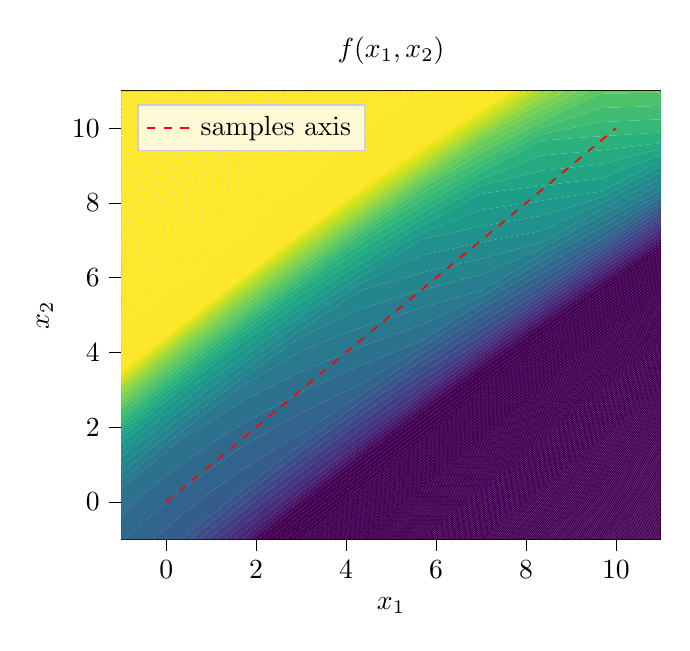
\begin{tikzpicture}

\definecolor{darkcyan30152138}{RGB}{30,152,138}
\definecolor{darkcyan30158136}{RGB}{30,158,136}
\definecolor{darkcyan32145140}{RGB}{32,145,140}
\definecolor{darkcyan34138141}{RGB}{34,138,141}
\definecolor{darkcyan36133141}{RGB}{36,133,141}
\definecolor{darkcyan39126142}{RGB}{39,126,142}
\definecolor{darkgray176}{RGB}{176,176,176}
\definecolor{darkslateblue5099141}{RGB}{50,99,141}
\definecolor{darkslateblue5393140}{RGB}{53,93,140}
\definecolor{darkslateblue5686139}{RGB}{56,86,139}
\definecolor{darkslateblue6078138}{RGB}{60,78,138}
\definecolor{darkslateblue6371136}{RGB}{63,71,136}
\definecolor{darkslateblue6662133}{RGB}{66,62,133}
\definecolor{darkslateblue6954129}{RGB}{69,54,129}
\definecolor{darkslateblue7047124}{RGB}{70,47,124}
\definecolor{darkslateblue7138118}{RGB}{71,38,118}
\definecolor{gold22822724}{RGB}{228,227,24}
\definecolor{gold24623031}{RGB}{246,230,31}
\definecolor{gold25323136}{RGB}{253,231,36}
\definecolor{greenyellow19422334}{RGB}{194,223,34}
\definecolor{greenyellow21022527}{RGB}{210,225,27}
\definecolor{indigo68184}{RGB}{68,1,84}
\definecolor{indigo70992}{RGB}{70,9,92}
\definecolor{indigo7120102}{RGB}{71,20,102}
\definecolor{indigo7229111}{RGB}{72,29,111}
\definecolor{lightgray204}{RGB}{204,204,204}
\definecolor{mediumseagreen10520491}{RGB}{105,204,91}
\definecolor{mediumseagreen32165133}{RGB}{32,165,133}
\definecolor{mediumseagreen37171129}{RGB}{37,171,129}
\definecolor{mediumseagreen43177125}{RGB}{43,177,125}
\definecolor{mediumseagreen53183120}{RGB}{53,183,120}
\definecolor{mediumseagreen64189114}{RGB}{64,189,114}
\definecolor{mediumseagreen77194107}{RGB}{77,194,107}
\definecolor{mediumseagreen9120098}{RGB}{91,200,98}
\definecolor{steelblue47106141}{RGB}{47,106,141}
\definecolor{teal41120142}{RGB}{41,120,142}
\definecolor{teal44113142}{RGB}{44,113,142}
\definecolor{yellowgreen12120981}{RGB}{121,209,81}
\definecolor{yellowgreen13921370}{RGB}{139,213,70}
\definecolor{yellowgreen15721758}{RGB}{157,217,58}
\definecolor{yellowgreen17522046}{RGB}{175,220,46}

\begin{axis}[
legend cell align={left},
legend style={
  fill opacity=0.8,
  draw opacity=1,
  text opacity=1,
  at={(0.03,0.97)},
  anchor=north west,
  draw=lightgray204
},
tick align=outside,
tick pos=left,
title={\(\displaystyle f(x_1, x_2)\)},
x grid style={darkgray176},
xlabel={\(\displaystyle x_1\)},
xmin=-1, xmax=11,
xtick style={color=black},
y grid style={darkgray176},
ylabel={\(\displaystyle x_2\)},
ymin=-1, ymax=11,
ytick style={color=black}
]
\addplot [draw=none, fill=indigo68184, forget plot]
table{%
x  y
11 -1
11 -0.997896213183731
10.997803806735 -1
11 -1
};
\addplot [draw=none, fill=indigo68184, forget plot]
table{%
x  y
11 -0.997896213183731
11 -0.964235624123422
10.9626647144949 -1
10.997803806735 -1
11 -0.997896213183731
};
\addplot [draw=none, fill=indigo68184, forget plot]
table{%
x  y
11 -0.964235624123422
11 -0.930575035063114
10.9275256222548 -1
10.9626647144949 -1
11 -0.964235624123422
};
\addplot [draw=none, fill=indigo68184, forget plot]
table{%
x  y
11 -0.930575035063114
11 -0.896914446002805
10.8923865300146 -1
10.9275256222548 -1
11 -0.930575035063114
};
\addplot [draw=none, fill=indigo68184, forget plot]
table{%
x  y
11 -0.896914446002805
11 -0.863253856942496
10.8572474377745 -1
10.8923865300146 -1
11 -0.896914446002805
};
\addplot [draw=none, fill=indigo68184, forget plot]
table{%
x  y
11 -0.863253856942496
11 -0.829593267882188
10.8221083455344 -1
10.8572474377745 -1
11 -0.863253856942496
};
\addplot [draw=none, fill=indigo68184, forget plot]
table{%
x  y
11 -0.829593267882188
11 -0.795932678821879
10.7869692532943 -1
10.8221083455344 -1
11 -0.829593267882188
};
\addplot [draw=none, fill=indigo68184, forget plot]
table{%
x  y
11 -0.795932678821879
11 -0.762272089761571
10.7518301610542 -1
10.7869692532943 -1
11 -0.795932678821879
};
\addplot [draw=none, fill=indigo68184, forget plot]
table{%
x  y
11 -0.762272089761571
11 -0.728611500701262
10.7166910688141 -1
10.7518301610542 -1
11 -0.762272089761571
};
\addplot [draw=none, fill=indigo68184, forget plot]
table{%
x  y
11 -0.728611500701262
11 -0.694950911640954
10.6815519765739 -1
10.7166910688141 -1
11 -0.728611500701262
};
\addplot [draw=none, fill=indigo68184, forget plot]
table{%
x  y
11 -0.694950911640954
11 -0.661290322580645
10.6464128843338 -1
10.6815519765739 -1
11 -0.694950911640954
};
\addplot [draw=none, fill=indigo68184, forget plot]
table{%
x  y
11 -0.661290322580645
11 -0.627629733520337
10.6112737920937 -1
10.6464128843338 -1
11 -0.661290322580645
};
\addplot [draw=none, fill=indigo68184, forget plot]
table{%
x  y
11 -0.627629733520337
11 -0.593969144460028
10.5761346998536 -1
10.6112737920937 -1
11 -0.627629733520337
};
\addplot [draw=none, fill=indigo68184, forget plot]
table{%
x  y
11 -0.593969144460028
11 -0.56030855539972
10.5409956076135 -1
10.5761346998536 -1
11 -0.593969144460028
};
\addplot [draw=none, fill=indigo68184, forget plot]
table{%
x  y
11 -0.56030855539972
11 -0.526647966339411
10.5058565153734 -1
10.5409956076135 -1
11 -0.56030855539972
};
\addplot [draw=none, fill=indigo68184, forget plot]
table{%
x  y
11 -0.526647966339411
11 -0.492987377279102
10.4707174231332 -1
10.5058565153734 -1
11 -0.526647966339411
};
\addplot [draw=none, fill=indigo68184, forget plot]
table{%
x  y
11 -0.492987377279102
11 -0.459326788218794
10.4355783308931 -1
10.4707174231332 -1
11 -0.492987377279102
};
\addplot [draw=none, fill=indigo68184, forget plot]
table{%
x  y
11 -0.459326788218794
11 -0.425666199158485
10.400439238653 -1
10.4355783308931 -1
11 -0.459326788218794
};
\addplot [draw=none, fill=indigo68184, forget plot]
table{%
x  y
11 -0.425666199158485
11 -0.392005610098177
10.3653001464129 -1
10.400439238653 -1
11 -0.425666199158485
};
\addplot [draw=none, fill=indigo68184, forget plot]
table{%
x  y
11 -0.392005610098177
11 -0.358345021037868
10.3301610541728 -1
10.3653001464129 -1
11 -0.392005610098177
};
\addplot [draw=none, fill=indigo68184, forget plot]
table{%
x  y
11 -0.358345021037868
11 -0.32468443197756
10.2950219619327 -1
10.3301610541728 -1
11 -0.358345021037868
};
\addplot [draw=none, fill=indigo68184, forget plot]
table{%
x  y
11 -0.32468443197756
11 -0.291023842917251
10.2598828696925 -1
10.2950219619327 -1
11 -0.32468443197756
};
\addplot [draw=none, fill=indigo68184, forget plot]
table{%
x  y
11 -0.291023842917251
11 -0.257363253856943
10.2247437774524 -1
10.2598828696925 -1
11 -0.291023842917251
};
\addplot [draw=none, fill=indigo68184, forget plot]
table{%
x  y
11 -0.257363253856943
11 -0.223702664796634
10.1896046852123 -1
10.2247437774524 -1
11 -0.257363253856943
};
\addplot [draw=none, fill=indigo68184, forget plot]
table{%
x  y
11 -0.223702664796634
11 -0.190042075736326
10.1544655929722 -1
10.1896046852123 -1
11 -0.223702664796634
};
\addplot [draw=none, fill=indigo68184, forget plot]
table{%
x  y
11 -0.190042075736326
11 -0.156381486676017
10.1193265007321 -1
10.1544655929722 -1
11 -0.190042075736326
};
\addplot [draw=none, fill=indigo68184, forget plot]
table{%
x  y
11 -0.156381486676017
11 -0.122720897615708
10.0841874084919 -1
10.1193265007321 -1
11 -0.156381486676017
};
\addplot [draw=none, fill=indigo68184, forget plot]
table{%
x  y
11 -0.122720897615708
11 -0.0890603085553999
10.0490483162518 -1
10.0841874084919 -1
11 -0.122720897615708
};
\addplot [draw=none, fill=indigo68184, forget plot]
table{%
x  y
11 -0.0890603085553999
11 -0.0553997194950913
10.0139092240117 -1
10.0490483162518 -1
11 -0.0890603085553999
};
\addplot [draw=none, fill=indigo68184, forget plot]
table{%
x  y
11 -0.0553997194950913
11 -0.0217391304347828
9.9787701317716 -1
10.0139092240117 -1
11 -0.0553997194950913
};
\addplot [draw=none, fill=indigo68184, forget plot]
table{%
x  y
11 -0.0217391304347828
11 0.0119214586255258
9.94363103953148 -1
9.9787701317716 -1
11 -0.0217391304347828
};
\addplot [draw=none, fill=indigo68184, forget plot]
table{%
x  y
11 0.0119214586255258
11 0.0455820476858343
9.90849194729136 -1
9.94363103953148 -1
11 0.0119214586255258
};
\addplot [draw=none, fill=indigo68184, forget plot]
table{%
x  y
11 0.0455820476858343
11 0.0792426367461429
9.87335285505124 -1
9.90849194729136 -1
11 0.0455820476858343
};
\addplot [draw=none, fill=indigo68184, forget plot]
table{%
x  y
11 0.0792426367461429
11 0.112903225806451
9.83821376281113 -1
9.87335285505124 -1
11 0.0792426367461429
};
\addplot [draw=none, fill=indigo68184, forget plot]
table{%
x  y
11 0.112903225806451
11 0.14656381486676
9.80307467057101 -1
9.83821376281113 -1
11 0.112903225806451
};
\addplot [draw=none, fill=indigo68184, forget plot]
table{%
x  y
11 0.14656381486676
11 0.180224403927069
9.76793557833089 -1
9.80307467057101 -1
11 0.14656381486676
};
\addplot [draw=none, fill=indigo68184, forget plot]
table{%
x  y
11 0.180224403927069
11 0.213884992987377
9.73279648609078 -1
9.76793557833089 -1
11 0.180224403927069
};
\addplot [draw=none, fill=indigo68184, forget plot]
table{%
x  y
11 0.213884992987377
11 0.247545582047686
9.69765739385066 -1
9.73279648609078 -1
11 0.213884992987377
};
\addplot [draw=none, fill=indigo68184, forget plot]
table{%
x  y
9.66666666666667 -1
9.69765739385066 -1
11 0.247545582047686
11 0.281206171107994
9.66666666666667 -0.995495495495495
9.66196793808734 -1
9.66666666666667 -1
};
\addplot [draw=none, fill=indigo68184, forget plot]
table{%
x  y
9.66666666666667 -0.995495495495495
11 0.281206171107994
11 0.314866760168303
9.66666666666667 -0.95733969263381
9.62216694306247 -1
9.66196793808734 -1
9.66666666666667 -0.995495495495495
};
\addplot [draw=none, fill=indigo68184, forget plot]
table{%
x  y
9.66666666666667 -0.95733969263381
11 0.314866760168303
11 0.333333333333333
11 0.350447604002106
10.9819143016138 0.333333333333333
9.66666666666667 -0.919183889772125
9.58236594803759 -1
9.62216694306247 -1
9.66666666666667 -0.95733969263381
};
\addplot [draw=none, fill=indigo68184, forget plot]
table{%
x  y
9.66666666666667 -0.919183889772125
10.9819143016138 0.333333333333333
11 0.350447604002106
11 0.388362295945234
10.9418475236505 0.333333333333333
9.66666666666667 -0.881028086910439
9.54256495301271 -1
9.58236594803759 -1
9.66666666666667 -0.919183889772125
};
\addplot [draw=none, fill=indigo68184, forget plot]
table{%
x  y
9.66666666666667 -0.881028086910439
10.9418475236505 0.333333333333333
11 0.388362295945234
11 0.426276987888362
10.9017807456873 0.333333333333333
9.66666666666666 -0.842872284048754
9.50276395798784 -1
9.54256495301271 -1
9.66666666666667 -0.881028086910439
};
\addplot [draw=none, fill=indigo68184, forget plot]
table{%
x  y
9.66666666666667 -0.842872284048754
10.9017807456873 0.333333333333333
11 0.426276987888362
11 0.46419167983149
10.861713967724 0.333333333333333
9.66666666666667 -0.804716481187069
9.46296296296296 -1
9.50276395798784 -1
9.66666666666667 -0.842872284048754
};
\addplot [draw=none, fill=indigo68184, forget plot]
table{%
x  y
9.66666666666667 -0.804716481187069
10.861713967724 0.333333333333333
11 0.46419167983149
11 0.502106371774618
10.8216471897607 0.333333333333333
9.66666666666667 -0.766560678325384
9.42316196793809 -1
9.46296296296296 -1
9.66666666666667 -0.804716481187069
};
\addplot [draw=none, fill=indigo68184, forget plot]
table{%
x  y
9.66666666666667 -0.766560678325384
10.8216471897607 0.333333333333333
11 0.502106371774618
11 0.540021063717746
10.7815804117974 0.333333333333333
9.66666666666667 -0.728404875463699
9.38336097291321 -1
9.42316196793809 -1
9.66666666666667 -0.766560678325384
};
\addplot [draw=none, fill=indigo68184, forget plot]
table{%
x  y
9.66666666666667 -0.728404875463699
10.7815804117974 0.333333333333333
11 0.540021063717746
11 0.577935755660874
10.7415136338342 0.333333333333333
9.66666666666667 -0.690249072602014
9.34355997788833 -1
9.38336097291321 -1
9.66666666666667 -0.728404875463699
};
\addplot [draw=none, fill=indigo68184, forget plot]
table{%
x  y
9.66666666666667 -0.690249072602014
10.7415136338342 0.333333333333333
11 0.577935755660874
11 0.615850447604002
10.7014468558709 0.333333333333333
9.66666666666667 -0.652093269740328
9.30375898286346 -1
9.34355997788833 -1
9.66666666666667 -0.690249072602014
};
\addplot [draw=none, fill=indigo68184, forget plot]
table{%
x  y
9.66666666666667 -0.652093269740328
10.7014468558709 0.333333333333333
11 0.615850447604002
11 0.65376513954713
10.6613800779076 0.333333333333333
9.66666666666667 -0.613937466878643
9.26395798783858 -1
9.30375898286346 -1
9.66666666666667 -0.652093269740328
};
\addplot [draw=none, fill=indigo68184, forget plot]
table{%
x  y
9.66666666666667 -0.613937466878643
10.6613800779076 0.333333333333333
11 0.65376513954713
11 0.691679831490258
10.6213132999444 0.333333333333333
9.66666666666666 -0.575781664016958
9.22415699281371 -1
9.26395798783858 -1
9.66666666666667 -0.613937466878643
};
\addplot [draw=none, fill=indigo68184, forget plot]
table{%
x  y
9.66666666666667 -0.575781664016958
10.6213132999444 0.333333333333333
11 0.691679831490258
11 0.729594523433386
10.5812465219811 0.333333333333333
9.66666666666667 -0.537625861155273
9.18435599778883 -1
9.22415699281371 -1
9.66666666666667 -0.575781664016958
};
\addplot [draw=none, fill=indigo68184, forget plot]
table{%
x  y
9.66666666666667 -0.537625861155273
10.5812465219811 0.333333333333333
11 0.729594523433386
11 0.767509215376514
10.5411797440178 0.333333333333333
9.66666666666667 -0.499470058293588
9.14455500276396 -1
9.18435599778883 -1
9.66666666666667 -0.537625861155273
};
\addplot [draw=none, fill=indigo68184, forget plot]
table{%
x  y
9.66666666666667 -0.499470058293588
10.5411797440178 0.333333333333333
11 0.767509215376514
11 0.805423907319642
10.5011129660545 0.333333333333333
9.66666666666667 -0.461314255431903
9.10475400773908 -1
9.14455500276396 -1
9.66666666666667 -0.499470058293588
};
\addplot [draw=none, fill=indigo68184, forget plot]
table{%
x  y
9.66666666666667 -0.461314255431903
10.5011129660545 0.333333333333333
11 0.805423907319642
11 0.84333859926277
10.4610461880913 0.333333333333333
9.66666666666667 -0.423158452570217
9.06495301271421 -1
9.10475400773908 -1
9.66666666666667 -0.461314255431903
};
\addplot [draw=none, fill=indigo68184, forget plot]
table{%
x  y
9.66666666666667 -0.423158452570217
10.4610461880913 0.333333333333333
11 0.84333859926277
11 0.881253291205898
10.420979410128 0.333333333333333
9.66666666666667 -0.385002649708532
9.02515201768933 -1
9.06495301271421 -1
9.66666666666667 -0.423158452570217
};
\addplot [draw=none, fill=indigo68184, forget plot]
table{%
x  y
9.66666666666667 -0.385002649708532
10.420979410128 0.333333333333333
11 0.881253291205898
11 0.919167983149026
10.3809126321647 0.333333333333333
9.66666666666667 -0.346846846846847
8.98535102266445 -1
9.02515201768933 -1
9.66666666666667 -0.385002649708532
};
\addplot [draw=none, fill=indigo68184, forget plot]
table{%
x  y
9.66666666666667 -0.346846846846847
10.3809126321647 0.333333333333333
11 0.919167983149026
11 0.957082675092154
10.3408458542014 0.333333333333333
9.66666666666667 -0.308691043985162
8.94555002763958 -1
8.98535102266445 -1
9.66666666666667 -0.346846846846847
};
\addplot [draw=none, fill=indigo68184, forget plot]
table{%
x  y
9.66666666666667 -0.308691043985162
10.3408458542014 0.333333333333333
11 0.957082675092154
11 0.994997367035282
10.3007790762382 0.333333333333333
9.66666666666667 -0.270535241123477
8.9057490326147 -1
8.94555002763958 -1
9.66666666666667 -0.308691043985162
};
\addplot [draw=none, fill=indigo68184, forget plot]
table{%
x  y
9.66666666666667 -0.270535241123477
10.3007790762382 0.333333333333333
11 0.994997367035282
11 1.03291205897841
10.2607122982749 0.333333333333333
9.66666666666667 -0.232379438261792
8.86594803758983 -1
8.9057490326147 -1
9.66666666666667 -0.270535241123477
};
\addplot [draw=none, fill=indigo68184, forget plot]
table{%
x  y
9.66666666666667 -0.232379438261792
10.2607122982749 0.333333333333333
11 1.03291205897841
11 1.07082675092154
10.2206455203116 0.333333333333333
9.66666666666667 -0.194223635400106
8.82614704256495 -1
8.86594803758983 -1
9.66666666666667 -0.232379438261792
};
\addplot [draw=none, fill=indigo68184, forget plot]
table{%
x  y
9.66666666666667 -0.194223635400106
10.2206455203116 0.333333333333333
11 1.07082675092154
11 1.10874144286467
10.1805787423484 0.333333333333333
9.66666666666667 -0.156067832538421
8.78634604754008 -1
8.82614704256495 -1
9.66666666666667 -0.194223635400106
};
\addplot [draw=none, fill=indigo68184, forget plot]
table{%
x  y
9.66666666666667 -0.156067832538421
10.1805787423484 0.333333333333333
11 1.10874144286467
11 1.14665613480779
10.1405119643851 0.333333333333333
9.66666666666667 -0.117912029676736
8.7465450525152 -1
8.78634604754008 -1
9.66666666666667 -0.156067832538421
};
\addplot [draw=none, fill=indigo68184, forget plot]
table{%
x  y
9.66666666666667 -0.117912029676736
10.1405119643851 0.333333333333333
11 1.14665613480779
11 1.18457082675092
10.1004451864218 0.333333333333333
9.66666666666667 -0.0797562268150508
8.70674405749033 -1
8.7465450525152 -1
9.66666666666667 -0.117912029676736
};
\addplot [draw=none, fill=indigo68184, forget plot]
table{%
x  y
9.66666666666666 -0.0797562268150509
10.1004451864218 0.333333333333333
11 1.18457082675092
11 1.22248551869405
10.0603784084585 0.333333333333333
9.66666666666667 -0.0416004239533657
8.66694306246545 -1
8.70674405749033 -1
9.66666666666666 -0.0797562268150509
};
\addplot [draw=none, fill=indigo68184, forget plot]
table{%
x  y
9.66666666666667 -0.0416004239533657
10.0603784084585 0.333333333333333
11 1.22248551869405
11 1.26040021063718
10.0203116304953 0.333333333333333
9.66666666666667 -0.00344462109168051
8.62714206744057 -1
8.66694306246545 -1
9.66666666666667 -0.0416004239533657
};
\addplot [draw=none, fill=indigo68184, forget plot]
table{%
x  y
9.66666666666667 -0.00344462109168051
10.0203116304953 0.333333333333333
11 1.26040021063718
11 1.29831490258031
9.980244852532 0.333333333333333
9.66666666666667 0.0347111817700047
8.5873410724157 -1
8.62714206744057 -1
9.66666666666667 -0.00344462109168051
};
\addplot [draw=none, fill=indigo68184, forget plot]
table{%
x  y
9.66666666666667 0.0347111817700047
9.980244852532 0.333333333333333
11 1.29831490258031
11 1.33622959452343
9.94017807456873 0.333333333333333
9.66666666666667 0.0728669846316898
8.54754007739082 -1
8.5873410724157 -1
9.66666666666667 0.0347111817700047
};
\addplot [draw=none, fill=indigo68184, forget plot]
table{%
x  y
9.66666666666667 0.0728669846316898
9.94017807456873 0.333333333333333
11 1.33622959452343
11 1.37414428646656
9.90011129660545 0.333333333333333
9.66666666666667 0.111022787493375
8.50773908236595 -1
8.54754007739082 -1
9.66666666666667 0.0728669846316898
};
\addplot [draw=none, fill=indigo68184, forget plot]
table{%
x  y
9.66666666666666 0.111022787493375
9.90011129660545 0.333333333333333
11 1.37414428646656
11 1.41205897840969
9.86004451864218 0.333333333333333
9.66666666666667 0.14917859035506
8.46793808734107 -1
8.50773908236595 -1
9.66666666666666 0.111022787493375
};
\addplot [draw=none, fill=indigo68184, forget plot]
table{%
x  y
9.66666666666667 0.14917859035506
9.86004451864218 0.333333333333333
11 1.41205897840969
11 1.44997367035282
9.81997774067891 0.333333333333333
9.66666666666667 0.187334393216745
8.4281370923162 -1
8.46793808734107 -1
9.66666666666667 0.14917859035506
};
\addplot [draw=none, fill=indigo68184, forget plot]
table{%
x  y
9.66666666666667 0.187334393216745
9.81997774067891 0.333333333333333
11 1.44997367035282
11 1.48788836229595
9.77991096271564 0.333333333333333
9.66666666666667 0.225490196078431
8.38833609729132 -1
8.4281370923162 -1
9.66666666666667 0.187334393216745
};
\addplot [draw=none, fill=indigo68184, forget plot]
table{%
x  y
9.66666666666667 0.22549019607843
9.77991096271564 0.333333333333333
11 1.48788836229595
11 1.52580305423907
9.73984418475236 0.333333333333333
9.66666666666667 0.263645998940116
8.34853510226645 -1
8.38833609729132 -1
9.66666666666667 0.22549019607843
};
\addplot [draw=none, fill=indigo68184, forget plot]
table{%
x  y
8.33333333333333 -1
8.34853510226645 -1
9.66666666666667 0.263645998940116
9.73984418475236 0.333333333333333
11 1.52580305423907
11 1.5637177461822
9.69977740678909 0.333333333333333
9.66666666666667 0.301801801801801
8.33333333333333 -0.972782874617738
8.30497131931166 -1
8.33333333333333 -1
};
\addplot [draw=none, fill=indigo68184, forget plot]
table{%
x  y
8.33333333333333 -0.972782874617738
9.66666666666666 0.301801801801801
9.69977740678909 0.333333333333333
11 1.5637177461822
11 1.60163243812533
9.66666666666667 0.340922890103217
9.65863840719332 0.333333333333333
8.33333333333333 -0.928746177370032
8.25908221797323 -1
8.30497131931166 -1
8.33333333333333 -0.972782874617738
};
\addplot [draw=none, fill=indigo68184, forget plot]
table{%
x  y
8.33333333333333 -0.928746177370032
9.65863840719332 0.333333333333333
9.66666666666667 0.340922890103217
11 1.60163243812533
11 1.63954713006846
9.66666666666667 0.384638737097752
9.61239563262685 0.333333333333333
8.33333333333333 -0.884709480122325
8.2131931166348 -1
8.25908221797323 -1
8.33333333333333 -0.928746177370032
};
\addplot [draw=none, fill=indigo68184, forget plot]
table{%
x  y
8.33333333333333 -0.884709480122325
9.61239563262685 0.333333333333333
9.66666666666667 0.384638737097752
11 1.63954713006846
11 1.66666666666667
11 1.67902350813743
10.9867313915858 1.66666666666667
9.66666666666667 0.428354584092288
9.56615285806037 0.333333333333333
8.33333333333333 -0.840672782874619
8.16730401529637 -1
8.2131931166348 -1
8.33333333333333 -0.884709480122325
};
\addplot [draw=none, fill=indigo68184, forget plot]
table{%
x  y
8.33333333333333 -0.840672782874619
9.56615285806037 0.333333333333333
9.66666666666667 0.428354584092288
10.9867313915858 1.66666666666667
11 1.67902350813743
11 1.72242314647378
10.9401294498382 1.66666666666667
9.66666666666667 0.472070431086823
9.5199100834939 0.333333333333333
8.33333333333333 -0.796636085626912
8.12141491395793 -1
8.16730401529637 -1
8.33333333333333 -0.840672782874619
};
\addplot [draw=none, fill=indigo68184, forget plot]
table{%
x  y
8.33333333333333 -0.796636085626912
9.5199100834939 0.333333333333333
9.66666666666667 0.472070431086823
10.9401294498382 1.66666666666667
11 1.72242314647378
11 1.76582278481013
10.8935275080906 1.66666666666667
9.66666666666667 0.515786278081359
9.47366730892742 0.333333333333333
8.33333333333333 -0.752599388379206
8.0755258126195 -1
8.12141491395793 -1
8.33333333333333 -0.796636085626912
};
\addplot [draw=none, fill=indigo68184, forget plot]
table{%
x  y
8.33333333333333 -0.752599388379206
9.47366730892742 0.333333333333333
9.66666666666667 0.515786278081359
10.8935275080906 1.66666666666667
11 1.76582278481013
11 1.80922242314647
10.846925566343 1.66666666666667
9.66666666666666 0.559502125075895
9.42742453436095 0.333333333333333
8.33333333333333 -0.7085626911315
8.02963671128107 -1
8.0755258126195 -1
8.33333333333333 -0.752599388379206
};
\addplot [draw=none, fill=indigo68184, forget plot]
table{%
x  y
8.33333333333333 -0.7085626911315
9.42742453436095 0.333333333333333
9.66666666666667 0.559502125075895
10.846925566343 1.66666666666667
11 1.80922242314647
11 1.85262206148282
10.8003236245955 1.66666666666667
9.66666666666667 0.60321797207043
9.38118175979448 0.333333333333333
8.33333333333333 -0.664525993883793
7.98374760994264 -1
8.02963671128107 -1
8.33333333333333 -0.7085626911315
};
\addplot [draw=none, fill=indigo68184, forget plot]
table{%
x  y
8.33333333333333 -0.664525993883793
9.38118175979448 0.333333333333333
9.66666666666667 0.60321797207043
10.8003236245955 1.66666666666667
11 1.85262206148282
11 1.89602169981917
10.7537216828479 1.66666666666667
9.66666666666667 0.646933819064966
9.334938985228 0.333333333333333
8.33333333333333 -0.620489296636087
7.93785850860421 -1
7.98374760994264 -1
8.33333333333333 -0.664525993883793
};
\addplot [draw=none, fill=indigo68184, forget plot]
table{%
x  y
8.33333333333333 -0.620489296636087
9.334938985228 0.333333333333333
9.66666666666667 0.646933819064966
10.7537216828479 1.66666666666667
11 1.89602169981917
11 1.93942133815552
10.7071197411003 1.66666666666667
9.66666666666666 0.690649666059501
9.28869621066153 0.333333333333333
8.33333333333333 -0.57645259938838
7.89196940726577 -1
7.93785850860421 -1
8.33333333333333 -0.620489296636087
};
\addplot [draw=none, fill=indigo68184, forget plot]
table{%
x  y
8.33333333333333 -0.57645259938838
9.28869621066153 0.333333333333333
9.66666666666667 0.690649666059501
10.7071197411003 1.66666666666667
11 1.93942133815552
11 1.98282097649186
10.6605177993527 1.66666666666667
9.66666666666667 0.734365513054037
9.24245343609505 0.333333333333333
8.33333333333333 -0.532415902140674
7.84608030592734 -1
7.89196940726577 -1
8.33333333333333 -0.57645259938838
};
\addplot [draw=none, fill=indigo68184, forget plot]
table{%
x  y
8.33333333333333 -0.532415902140674
9.24245343609505 0.333333333333333
9.66666666666667 0.734365513054037
10.6605177993527 1.66666666666667
11 1.98282097649186
11 2.02622061482821
10.6139158576052 1.66666666666667
9.66666666666666 0.778081360048572
9.19621066152858 0.333333333333333
8.33333333333333 -0.488379204892967
7.80019120458891 -1
7.84608030592734 -1
8.33333333333333 -0.532415902140674
};
\addplot [draw=none, fill=indigo68184, forget plot]
table{%
x  y
8.33333333333333 -0.488379204892967
9.19621066152858 0.333333333333333
9.66666666666667 0.778081360048572
10.6139158576052 1.66666666666667
11 2.02622061482821
11 2.06962025316456
10.5673139158576 1.66666666666667
9.66666666666667 0.821797207043108
9.14996788696211 0.333333333333333
8.33333333333333 -0.444342507645261
7.75430210325048 -1
7.80019120458891 -1
8.33333333333333 -0.488379204892967
};
\addplot [draw=none, fill=indigo68184, forget plot]
table{%
x  y
8.33333333333333 -0.444342507645261
9.14996788696211 0.333333333333333
9.66666666666667 0.821797207043108
10.5673139158576 1.66666666666667
11 2.06962025316456
11 2.1130198915009
10.52071197411 1.66666666666667
9.66666666666666 0.865513054037643
9.10372511239563 0.333333333333333
8.33333333333333 -0.400305810397555
7.70841300191205 -1
7.75430210325048 -1
8.33333333333333 -0.444342507645261
};
\addplot [draw=none, fill=indigo68184, forget plot]
table{%
x  y
8.33333333333333 -0.400305810397555
9.10372511239563 0.333333333333333
9.66666666666667 0.865513054037643
10.52071197411 1.66666666666667
11 2.1130198915009
11 2.15641952983725
10.4741100323625 1.66666666666667
9.66666666666666 0.909228901032179
9.05748233782916 0.333333333333333
8.33333333333333 -0.356269113149848
7.66252390057361 -1
7.70841300191205 -1
8.33333333333333 -0.400305810397555
};
\addplot [draw=none, fill=indigo68184, forget plot]
table{%
x  y
8.33333333333333 -0.356269113149848
9.05748233782916 0.333333333333333
9.66666666666667 0.909228901032179
10.4741100323625 1.66666666666667
11 2.15641952983725
11 2.1998191681736
10.4275080906149 1.66666666666667
9.66666666666666 0.952944748026715
9.01123956326268 0.333333333333333
8.33333333333333 -0.312232415902142
7.61663479923518 -1
7.66252390057361 -1
8.33333333333333 -0.356269113149848
};
\addplot [draw=none, fill=indigo68184, forget plot]
table{%
x  y
8.33333333333333 -0.312232415902142
9.01123956326268 0.333333333333333
9.66666666666667 0.952944748026714
10.4275080906149 1.66666666666667
11 2.1998191681736
11 2.24321880650995
10.3809061488673 1.66666666666667
9.66666666666666 0.99666059502125
8.96499678869621 0.333333333333333
8.33333333333333 -0.268195718654435
7.57074569789675 -1
7.61663479923518 -1
8.33333333333333 -0.312232415902142
};
\addplot [draw=none, fill=indigo68184, forget plot]
table{%
x  y
8.33333333333333 -0.268195718654435
8.96499678869621 0.333333333333333
9.66666666666667 0.99666059502125
10.3809061488673 1.66666666666667
11 2.24321880650995
11 2.28661844484629
10.3343042071197 1.66666666666667
9.66666666666667 1.04037644201579
8.91875401412974 0.333333333333333
8.33333333333333 -0.224159021406729
7.52485659655832 -1
7.57074569789675 -1
8.33333333333333 -0.268195718654435
};
\addplot [draw=none, fill=indigo68184, forget plot]
table{%
x  y
8.33333333333333 -0.224159021406729
8.91875401412974 0.333333333333333
9.66666666666667 1.04037644201579
10.3343042071197 1.66666666666667
11 2.28661844484629
11 2.33001808318264
10.2877022653722 1.66666666666667
9.66666666666667 1.08409228901032
8.87251123956326 0.333333333333333
8.33333333333333 -0.180122324159023
7.47896749521989 -1
7.52485659655832 -1
8.33333333333333 -0.224159021406729
};
\addplot [draw=none, fill=indigo68184, forget plot]
table{%
x  y
8.33333333333333 -0.180122324159022
8.87251123956326 0.333333333333333
9.66666666666667 1.08409228901032
10.2877022653722 1.66666666666667
11 2.33001808318264
11 2.37341772151899
10.2411003236246 1.66666666666667
9.66666666666667 1.12780813600486
8.82626846499679 0.333333333333333
8.33333333333333 -0.136085626911316
7.43307839388145 -1
7.47896749521989 -1
8.33333333333333 -0.180122324159022
};
\addplot [draw=none, fill=indigo68184, forget plot]
table{%
x  y
8.33333333333333 -0.136085626911316
8.82626846499679 0.333333333333333
9.66666666666667 1.12780813600486
10.2411003236246 1.66666666666667
11 2.37341772151899
11 2.41681735985533
10.194498381877 1.66666666666667
9.66666666666667 1.17152398299939
8.78002569043031 0.333333333333333
8.33333333333333 -0.0920489296636095
7.38718929254302 -1
7.43307839388145 -1
8.33333333333333 -0.136085626911316
};
\addplot [draw=none, fill=indigo68184, forget plot]
table{%
x  y
8.33333333333333 -0.0920489296636096
8.78002569043031 0.333333333333333
9.66666666666667 1.17152398299939
10.194498381877 1.66666666666667
11 2.41681735985533
11 2.46021699819168
10.1478964401294 1.66666666666667
9.66666666666667 1.21523982999393
8.73378291586384 0.333333333333333
8.33333333333333 -0.0480122324159031
7.34130019120459 -1
7.38718929254302 -1
8.33333333333333 -0.0920489296636096
};
\addplot [draw=none, fill=indigo68184, forget plot]
table{%
x  y
8.33333333333333 -0.0480122324159032
8.73378291586384 0.333333333333333
9.66666666666667 1.21523982999393
10.1478964401294 1.66666666666667
11 2.46021699819168
11 2.50361663652803
10.1012944983819 1.66666666666667
9.66666666666667 1.25895567698846
8.68754014129737 0.333333333333333
8.33333333333333 -0.00397553516819668
7.29541108986616 -1
7.34130019120459 -1
8.33333333333333 -0.0480122324159032
};
\addplot [draw=none, fill=indigo68184, forget plot]
table{%
x  y
8.33333333333333 -0.00397553516819679
8.68754014129737 0.333333333333333
9.66666666666667 1.25895567698846
10.1012944983819 1.66666666666667
11 2.50361663652803
11 2.54701627486438
10.0546925566343 1.66666666666667
9.66666666666667 1.302671523983
8.64129736673089 0.333333333333333
8.33333333333333 0.0400611620795097
7.24952198852773 -1
7.29541108986616 -1
8.33333333333333 -0.00397553516819679
};
\addplot [draw=none, fill=indigo68184, forget plot]
table{%
x  y
8.33333333333333 0.0400611620795097
8.64129736673089 0.333333333333333
9.66666666666667 1.302671523983
10.0546925566343 1.66666666666667
11 2.54701627486438
11 2.59041591320072
10.0080906148867 1.66666666666667
9.66666666666667 1.34638737097753
8.59505459216442 0.333333333333333
8.33333333333333 0.0840978593272161
7.20363288718929 -1
7.24952198852773 -1
8.33333333333333 0.0400611620795097
};
\addplot [draw=none, fill=indigo68184, forget plot]
table{%
x  y
8.33333333333333 0.0840978593272161
8.59505459216442 0.333333333333333
9.66666666666667 1.34638737097753
10.0080906148867 1.66666666666667
11 2.59041591320072
11 2.63381555153707
9.96148867313916 1.66666666666667
9.66666666666667 1.39010321797207
8.54881181759795 0.333333333333333
8.33333333333333 0.128134556574923
7.15774378585086 -1
7.20363288718929 -1
8.33333333333333 0.0840978593272161
};
\addplot [draw=none, fill=indigo68184, forget plot]
table{%
x  y
8.33333333333333 0.128134556574923
8.54881181759794 0.333333333333333
9.66666666666667 1.39010321797207
9.96148867313916 1.66666666666667
11 2.63381555153707
11 2.67721518987342
9.91488673139158 1.66666666666667
9.66666666666667 1.43381906496661
8.50256904303147 0.333333333333333
8.33333333333333 0.172171253822629
7.11185468451243 -1
7.15774378585086 -1
8.33333333333333 0.128134556574923
};
\addplot [draw=none, fill=indigo68184, forget plot]
table{%
x  y
8.33333333333333 0.172171253822629
8.50256904303147 0.333333333333333
9.66666666666667 1.43381906496661
9.91488673139158 1.66666666666667
11 2.67721518987342
11 2.72061482820977
9.86828478964401 1.66666666666667
9.66666666666667 1.47753491196114
8.456326268465 0.333333333333333
8.33333333333333 0.216207951070335
7.065965583174 -1
7.11185468451243 -1
8.33333333333333 0.172171253822629
};
\addplot [draw=none, fill=indigo68184, forget plot]
table{%
x  y
8.33333333333333 0.216207951070335
8.456326268465 0.333333333333333
9.66666666666667 1.47753491196114
9.86828478964401 1.66666666666667
11 2.72061482820977
11 2.76401446654611
9.82168284789644 1.66666666666667
9.66666666666667 1.52125075895568
8.41008349389852 0.333333333333333
8.33333333333333 0.260244648318042
7.02007648183556 -1
7.065965583174 -1
8.33333333333333 0.216207951070335
};
\addplot [draw=none, fill=indigo68184, forget plot]
table{%
x  y
7 -1
7.02007648183556 -1
8.33333333333333 0.260244648318042
8.41008349389852 0.333333333333333
9.66666666666667 1.52125075895568
9.82168284789644 1.66666666666667
11 2.76401446654611
11 2.80741410488246
9.77508090614887 1.66666666666667
9.66666666666667 1.56496660595021
8.36384071933205 0.333333333333333
8.33333333333333 0.304281345565748
7 -0.970715835140998
6.96952595936795 -1
7 -1
};
\addplot [draw=none, fill=indigo68184, forget plot]
table{%
x  y
7 -0.970715835140998
8.33333333333333 0.304281345565748
8.36384071933205 0.333333333333333
9.66666666666667 1.56496660595021
9.77508090614887 1.66666666666667
11 2.80741410488246
11 2.85081374321881
9.72847896440129 1.66666666666667
9.66666666666667 1.60868245294475
8.33333333333333 0.350896057347669
8.31473044798785 0.333333333333333
7 -0.918655097613883
6.91534988713318 -1
6.96952595936795 -1
7 -0.970715835140998
};
\addplot [draw=none, fill=indigo68184, forget plot]
table{%
x  y
7 -0.918655097613883
8.31473044798785 0.333333333333333
8.33333333333333 0.350896057347669
9.66666666666667 1.60868245294475
9.72847896440129 1.66666666666667
11 2.85081374321881
11 2.89421338155515
9.68187702265372 1.66666666666667
9.66666666666667 1.65239829993928
8.33333333333333 0.402508960573476
8.26006074411541 0.333333333333333
7 -0.866594360086768
6.86117381489842 -1
6.91534988713318 -1
7 -0.918655097613883
};
\addplot [draw=none, fill=indigo68184, forget plot]
table{%
x  y
7 -0.866594360086768
8.26006074411541 0.333333333333333
8.33333333333333 0.402508960573476
9.66666666666667 1.65239829993928
9.68187702265372 1.66666666666667
11 2.89421338155515
11 2.9376130198915
9.66666666666667 1.70113717128642
9.62950191570881 1.66666666666667
8.33333333333333 0.454121863799282
8.20539104024298 0.333333333333333
7 -0.814533622559653
6.80699774266366 -1
6.86117381489842 -1
7 -0.866594360086768
};
\addplot [draw=none, fill=indigo68184, forget plot]
table{%
x  y
7 -0.814533622559653
8.20539104024298 0.333333333333333
8.33333333333333 0.454121863799282
9.62950191570881 1.66666666666667
9.66666666666667 1.70113717128642
11 2.9376130198915
11 2.98101265822785
9.66666666666667 1.75230987917555
9.57432950191571 1.66666666666667
8.33333333333333 0.505734767025088
8.15072133637054 0.333333333333333
7 -0.762472885032538
6.75282167042889 -1
6.80699774266366 -1
7 -0.814533622559653
};
\addplot [draw=none, fill=indigo68184, forget plot]
table{%
x  y
7 -0.762472885032538
8.15072133637054 0.333333333333333
8.33333333333333 0.505734767025088
9.57432950191571 1.66666666666667
9.66666666666667 1.75230987917555
11 2.98101265822785
11 3
11 3.02854122621564
10.9686774941995 3
9.66666666666667 1.80348258706468
9.5191570881226 1.66666666666667
8.33333333333333 0.557347670250895
8.0960516324981 0.333333333333333
7 -0.710412147505423
6.69864559819413 -1
6.75282167042889 -1
7 -0.762472885032538
};
\addplot [draw=none, fill=indigo68184, forget plot]
table{%
x  y
7 -0.710412147505423
8.0960516324981 0.333333333333333
8.33333333333333 0.557347670250895
9.5191570881226 1.66666666666667
9.66666666666667 1.80348258706468
10.9686774941995 3
11 3.02854122621564
11 3.07928118393235
10.9129930394432 3
9.66666666666667 1.8546552949538
9.4639846743295 1.66666666666667
8.33333333333333 0.608960573476701
8.04138192862566 0.333333333333333
7 -0.658351409978308
6.64446952595937 -1
6.69864559819413 -1
7 -0.710412147505423
};
\addplot [draw=none, fill=indigo68184, forget plot]
table{%
x  y
7 -0.658351409978308
8.04138192862566 0.333333333333333
8.33333333333333 0.608960573476701
9.4639846743295 1.66666666666667
9.66666666666667 1.8546552949538
10.9129930394432 3
11 3.07928118393235
11 3.13002114164905
10.8573085846868 3
9.66666666666667 1.90582800284293
9.4088122605364 1.66666666666667
8.33333333333333 0.660573476702508
7.98671222475323 0.333333333333333
7 -0.606290672451193
6.5902934537246 -1
6.64446952595937 -1
7 -0.658351409978308
};
\addplot [draw=none, fill=indigo68184, forget plot]
table{%
x  y
7 -0.606290672451193
7.98671222475323 0.333333333333333
8.33333333333333 0.660573476702508
9.4088122605364 1.66666666666667
9.66666666666667 1.90582800284293
10.8573085846868 3
11 3.13002114164905
11 3.18076109936575
10.8016241299304 3
9.66666666666667 1.95700071073205
9.35363984674329 1.66666666666667
8.33333333333333 0.712186379928314
7.93204252088079 0.333333333333333
7 -0.554229934924078
6.53611738148984 -1
6.5902934537246 -1
7 -0.606290672451193
};
\addplot [draw=none, fill=indigo68184, forget plot]
table{%
x  y
7 -0.554229934924078
7.93204252088079 0.333333333333333
8.33333333333333 0.712186379928314
9.3536398467433 1.66666666666667
9.66666666666667 1.95700071073205
10.8016241299304 3
11 3.18076109936575
11 3.23150105708245
10.745939675174 3
9.66666666666667 2.00817341862118
9.29846743295019 1.66666666666667
8.33333333333333 0.763799283154121
7.87737281700835 0.333333333333333
7 -0.502169197396963
6.48194130925508 -1
6.53611738148984 -1
7 -0.554229934924078
};
\addplot [draw=none, fill=indigo68184, forget plot]
table{%
x  y
7 -0.502169197396963
7.87737281700835 0.333333333333333
8.33333333333333 0.763799283154121
9.29846743295019 1.66666666666667
9.66666666666667 2.00817341862118
10.745939675174 3
11 3.23150105708245
11 3.28224101479915
10.6902552204176 3
9.66666666666667 2.05934612651031
9.24329501915709 1.66666666666667
8.33333333333333 0.815412186379927
7.82270311313592 0.333333333333333
7 -0.450108459869848
6.42776523702032 -1
6.48194130925508 -1
7 -0.502169197396963
};
\addplot [draw=none, fill=indigo68184, forget plot]
table{%
x  y
7 -0.450108459869848
7.82270311313591 0.333333333333333
8.33333333333333 0.815412186379927
9.24329501915709 1.66666666666667
9.66666666666667 2.05934612651031
10.6902552204176 3
11 3.28224101479915
11 3.33298097251586
10.6345707656613 3
9.66666666666667 2.11051883439943
9.18812260536398 1.66666666666667
8.33333333333333 0.867025089605734
7.76803340926348 0.333333333333333
7 -0.398047722342733
6.37358916478555 -1
6.42776523702032 -1
7 -0.450108459869848
};
\addplot [draw=none, fill=indigo68184, forget plot]
table{%
x  y
7 -0.398047722342733
7.76803340926348 0.333333333333333
8.33333333333333 0.867025089605734
9.18812260536398 1.66666666666667
9.66666666666667 2.11051883439943
10.6345707656613 3
11 3.33298097251586
11 3.38372093023256
10.5788863109049 3
9.66666666666666 2.16169154228856
9.13295019157088 1.66666666666667
8.33333333333333 0.91863799283154
7.71336370539104 0.333333333333333
7 -0.345986984815618
6.31941309255079 -1
6.37358916478555 -1
7 -0.398047722342733
};
\addplot [draw=none, fill=indigo68184, forget plot]
table{%
x  y
7 -0.345986984815618
7.71336370539104 0.333333333333333
8.33333333333333 0.91863799283154
9.13295019157088 1.66666666666667
9.66666666666667 2.16169154228856
10.5788863109049 3
11 3.38372093023256
11 3.43446088794926
10.5232018561485 3
9.66666666666667 2.21286425017768
9.07777777777778 1.66666666666667
8.33333333333333 0.970250896057347
7.6586940015186 0.333333333333333
7 -0.293926247288503
6.26523702031603 -1
6.31941309255079 -1
7 -0.345986984815618
};
\addplot [draw=none, fill=indigo68184, forget plot]
table{%
x  y
7 -0.293926247288503
7.6586940015186 0.333333333333333
8.33333333333333 0.970250896057347
9.07777777777778 1.66666666666667
9.66666666666667 2.21286425017768
10.5232018561485 3
11 3.43446088794926
11 3.48520084566596
10.4675174013921 3
9.66666666666667 2.26403695806681
9.02260536398467 1.66666666666667
8.33333333333333 1.02186379928315
7.60402429764616 0.333333333333333
7 -0.241865509761388
6.21106094808126 -1
6.26523702031603 -1
7 -0.293926247288503
};
\addplot [draw=none, fill=indigo68184, forget plot]
table{%
x  y
7 -0.241865509761388
7.60402429764616 0.333333333333333
8.33333333333333 1.02186379928315
9.02260536398467 1.66666666666667
9.66666666666667 2.26403695806681
10.4675174013921 3
11 3.48520084566596
11 3.53594080338266
10.4118329466357 3
9.66666666666667 2.31520966595593
8.96743295019157 1.66666666666667
8.33333333333333 1.07347670250896
7.54935459377373 0.333333333333333
7 -0.189804772234273
6.1568848758465 -1
6.21106094808126 -1
7 -0.241865509761388
};
\addplot [draw=none, fill=indigo68184, forget plot]
table{%
x  y
7 -0.189804772234273
7.54935459377373 0.333333333333333
8.33333333333333 1.07347670250896
8.96743295019157 1.66666666666667
9.66666666666667 2.31520966595593
10.4118329466357 3
11 3.53594080338266
11 3.58668076109937
10.3561484918794 3
9.66666666666667 2.36638237384506
8.91226053639847 1.66666666666667
8.33333333333333 1.12508960573477
7.49468488990129 0.333333333333333
7 -0.137744034707158
6.10270880361174 -1
6.1568848758465 -1
7 -0.189804772234273
};
\addplot [draw=none, fill=indigo68184, forget plot]
table{%
x  y
7 -0.137744034707158
7.49468488990129 0.333333333333333
8.33333333333333 1.12508960573477
8.91226053639847 1.66666666666667
9.66666666666667 2.36638237384506
10.3561484918794 3
11 3.58668076109937
11 3.63742071881607
10.300464037123 3
9.66666666666667 2.41755508173419
8.85708812260536 1.66666666666667
8.33333333333333 1.17670250896057
7.44001518602885 0.333333333333333
7 -0.0856832971800431
6.04853273137697 -1
6.10270880361174 -1
7 -0.137744034707158
};
\addplot [draw=none, fill=indigo68184, forget plot]
table{%
x  y
7 -0.085683297180043
7.44001518602885 0.333333333333333
8.33333333333333 1.17670250896057
8.85708812260536 1.66666666666667
9.66666666666667 2.41755508173419
10.300464037123 3
11 3.63742071881607
11 3.68816067653277
10.2447795823666 3
9.66666666666667 2.46872778962331
8.80191570881226 1.66666666666667
8.33333333333333 1.22831541218638
7.38534548215642 0.333333333333333
7 -0.033622559652928
5.99435665914221 -1
6.04853273137697 -1
7 -0.085683297180043
};
\addplot [draw=none, fill=indigo68184, forget plot]
table{%
x  y
7 -0.033622559652928
7.38534548215642 0.333333333333333
8.33333333333333 1.22831541218638
8.80191570881226 1.66666666666667
9.66666666666667 2.46872778962331
10.2447795823666 3
11 3.68816067653277
11 3.73890063424947
10.1890951276102 3
9.66666666666667 2.51990049751244
8.74674329501916 1.66666666666667
8.33333333333333 1.27992831541219
7.33067577828398 0.333333333333333
7 0.0184381778741869
5.94018058690745 -1
5.99435665914221 -1
7 -0.033622559652928
};
\addplot [draw=none, fill=indigo68184, forget plot]
table{%
x  y
7 0.0184381778741869
7.33067577828398 0.333333333333333
8.33333333333333 1.27992831541219
8.74674329501916 1.66666666666667
9.66666666666667 2.51990049751244
10.1890951276102 3
11 3.73890063424947
11 3.78964059196617
10.1334106728538 3
9.66666666666667 2.57107320540156
8.69157088122605 1.66666666666667
8.33333333333333 1.33154121863799
7.27600607441154 0.333333333333333
7 0.070498915401302
5.88600451467269 -1
5.94018058690745 -1
7 0.0184381778741869
};
\addplot [draw=none, fill=indigo68184, forget plot]
table{%
x  y
7 0.0704989154013019
7.27600607441154 0.333333333333333
8.33333333333333 1.33154121863799
8.69157088122605 1.66666666666667
9.66666666666667 2.57107320540156
10.1334106728538 3
11 3.78964059196617
11 3.84038054968288
10.0777262180974 3
9.66666666666667 2.62224591329069
8.63639846743295 1.66666666666667
8.33333333333333 1.3831541218638
7.2213363705391 0.333333333333333
7 0.122559652928417
5.83182844243792 -1
5.88600451467269 -1
7 0.0704989154013019
};
\addplot [draw=none, fill=indigo68184, forget plot]
table{%
x  y
7 0.122559652928417
7.2213363705391 0.333333333333333
8.33333333333333 1.3831541218638
8.63639846743295 1.66666666666667
9.66666666666667 2.62224591329069
10.0777262180974 3
11 3.84038054968288
11 3.89112050739958
10.0220417633411 3
9.66666666666667 2.67341862117981
8.58122605363985 1.66666666666667
8.33333333333333 1.4347670250896
7.16666666666667 0.333333333333333
7 0.174620390455532
5.77765237020316 -1
5.83182844243792 -1
7 0.122559652928417
};
\addplot [draw=none, fill=indigo68184, forget plot]
table{%
x  y
7 0.174620390455532
7.16666666666667 0.333333333333333
8.33333333333333 1.4347670250896
8.58122605363985 1.66666666666667
9.66666666666666 2.67341862117981
10.0220417633411 3
11 3.89112050739958
11 3.94186046511628
9.96635730858469 3
9.66666666666667 2.72459132906894
8.52605363984674 1.66666666666667
8.33333333333333 1.48637992831541
7.11199696279423 0.333333333333333
7 0.226681127982647
5.7234762979684 -1
5.77765237020316 -1
7 0.174620390455532
};
\addplot [draw=none, fill=indigo68184, forget plot]
table{%
x  y
7 0.226681127982647
7.11199696279423 0.333333333333333
8.33333333333333 1.48637992831541
8.52605363984674 1.66666666666667
9.66666666666667 2.72459132906894
9.96635730858469 3
11 3.94186046511628
11 3.99260042283298
9.91067285382831 3
9.66666666666667 2.77576403695807
8.47088122605364 1.66666666666667
8.33333333333333 1.53799283154122
7.05732725892179 0.333333333333333
7 0.278741865509762
5.66930022573363 -1
5.7234762979684 -1
7 0.226681127982647
};
\addplot [draw=none, fill=indigo68184, forget plot]
table{%
x  y
5.66666666666667 -1
5.66930022573363 -1
7 0.278741865509762
7.05732725892179 0.333333333333333
8.33333333333333 1.53799283154122
8.47088122605364 1.66666666666667
9.66666666666666 2.77576403695807
9.91067285382831 3
11 3.99260042283298
11 4.04334038054968
9.85498839907192 3
9.66666666666667 2.82693674484719
8.41570881226054 1.66666666666667
8.33333333333333 1.58960573476702
7.00265755504935 0.333333333333333
7 0.330802603036877
5.66666666666667 -0.939434129089302
5.60376492194674 -1
5.66666666666667 -1
};
\addplot [draw=none, fill=indigo68184, forget plot]
table{%
x  y
5.66666666666667 -0.939434129089302
7 0.330802603036877
7.00265755504935 0.333333333333333
8.33333333333333 1.58960573476702
8.41570881226054 1.66666666666667
9.66666666666667 2.82693674484719
9.85498839907192 3
11 4.04334038054968
11 4.09408033826638
9.79930394431554 3
9.66666666666667 2.87810945273632
8.36053639846743 1.66666666666667
8.33333333333333 1.64121863799283
7 0.39326334208224
6.9363974001857 0.333333333333333
5.66666666666667 -0.875773651635721
5.5376492194674 -1
5.60376492194674 -1
5.66666666666667 -0.939434129089302
};
\addplot [draw=none, fill=indigo68184, forget plot]
table{%
x  y
5.66666666666667 -0.875773651635721
6.9363974001857 0.333333333333333
7 0.39326334208224
8.33333333333333 1.64121863799283
8.36053639846743 1.66666666666667
9.66666666666667 2.87810945273632
9.79930394431554 3
11 4.09408033826638
11 4.14482029598309
9.74361948955917 3
9.66666666666667 2.92928216062544
8.33333333333333 1.6982683982684
8.29906103286385 1.66666666666667
7 0.456255468066492
6.86954503249768 0.333333333333333
5.66666666666667 -0.81211317418214
5.47153351698806 -1
5.5376492194674 -1
5.66666666666667 -0.875773651635721
};
\addplot [draw=none, fill=indigo68184, forget plot]
table{%
x  y
5.66666666666667 -0.81211317418214
6.86954503249768 0.333333333333333
7 0.456255468066492
8.29906103286385 1.66666666666667
8.33333333333333 1.6982683982684
9.66666666666667 2.92928216062544
9.74361948955917 3
11 4.14482029598309
11 4.19556025369979
9.68793503480278 3
9.66666666666667 2.98045486851457
8.33333333333333 1.76060606060606
8.23145539906103 1.66666666666667
7 0.519247594050744
6.80269266480966 0.333333333333333
5.66666666666667 -0.748452696728559
5.40541781450872 -1
5.47153351698806 -1
5.66666666666667 -0.81211317418214
};
\addplot [draw=none, fill=indigo68184, forget plot]
table{%
x  y
5.66666666666667 -0.748452696728559
6.80269266480966 0.333333333333333
7 0.519247594050744
8.23145539906103 1.66666666666667
8.33333333333333 1.76060606060606
9.66666666666667 2.98045486851457
9.68793503480278 3
11 4.19556025369979
11 4.24630021141649
9.66666666666667 3.03813196229649
9.62440645773979 3
8.33333333333333 1.82294372294372
8.16384976525822 1.66666666666667
7 0.582239720034996
6.73584029712163 0.333333333333333
5.66666666666667 -0.684792219274978
5.33930211202938 -1
5.40541781450872 -1
5.66666666666667 -0.748452696728559
};
\addplot [draw=none, fill=indigo68184, forget plot]
table{%
x  y
5.66666666666667 -0.684792219274978
6.73584029712163 0.333333333333333
7 0.582239720034996
8.16384976525822 1.66666666666667
8.33333333333333 1.82294372294372
9.62440645773979 3
9.66666666666667 3.03813196229649
11 4.24630021141649
11 4.29704016913319
9.66666666666667 3.09982862039417
9.55603038936372 3
8.33333333333333 1.88528138528138
8.0962441314554 1.66666666666667
7 0.645231846019248
6.66898792943361 0.333333333333333
5.66666666666667 -0.621131741821398
5.27318640955005 -1
5.33930211202938 -1
5.66666666666667 -0.684792219274978
};
\addplot [draw=none, fill=indigo68184, forget plot]
table{%
x  y
5.66666666666667 -0.621131741821398
6.66898792943361 0.333333333333333
7 0.645231846019248
8.0962441314554 1.66666666666667
8.33333333333333 1.88528138528138
9.55603038936372 3
9.66666666666667 3.09982862039417
11 4.29704016913319
11 4.33333333333333
11 4.35072094995759
10.9803073967339 4.33333333333333
9.66666666666667 3.16152527849186
9.48765432098766 3
8.33333333333333 1.94761904761905
8.02863849765258 1.66666666666667
7 0.7082239720035
6.60213556174559 0.333333333333333
5.66666666666667 -0.557471264367817
5.20707070707071 -1
5.27318640955005 -1
5.66666666666667 -0.621131741821398
};
\addplot [draw=none, fill=indigo68184, forget plot]
table{%
x  y
5.66666666666667 -0.557471264367817
6.60213556174559 0.333333333333333
7 0.7082239720035
8.02863849765258 1.66666666666667
8.33333333333333 1.94761904761905
9.48765432098766 3
9.66666666666667 3.16152527849186
10.9803073967339 4.33333333333333
11 4.35072094995759
11 4.41178965224767
10.9111431316042 4.33333333333333
9.66666666666667 3.22322193658955
9.41927825261159 3
8.33333333333333 2.00995670995671
7.96103286384977 1.66666666666667
7 0.771216097987752
6.53528319405757 0.333333333333333
5.66666666666667 -0.493810786914236
5.14095500459137 -1
5.20707070707071 -1
5.66666666666667 -0.557471264367817
};
\addplot [draw=none, fill=indigo68184, forget plot]
table{%
x  y
5.66666666666667 -0.493810786914236
6.53528319405757 0.333333333333333
7 0.771216097987752
7.96103286384977 1.66666666666667
8.33333333333333 2.00995670995671
9.41927825261159 3
9.66666666666667 3.22322193658955
10.9111431316042 4.33333333333333
11 4.41178965224767
11 4.47285835453774
10.8419788664745 4.33333333333333
9.66666666666667 3.28491859468723
9.35090218423552 3
8.33333333333333 2.07229437229437
7.89342723004695 1.66666666666667
7 0.834208223972004
6.46843082636954 0.333333333333333
5.66666666666667 -0.430150309460655
5.07483930211203 -1
5.14095500459137 -1
5.66666666666667 -0.493810786914236
};
\addplot [draw=none, fill=indigo68184, forget plot]
table{%
x  y
5.66666666666667 -0.430150309460655
6.46843082636954 0.333333333333333
7 0.834208223972004
7.89342723004695 1.66666666666667
8.33333333333333 2.07229437229437
9.35090218423552 3
9.66666666666667 3.28491859468723
10.8419788664745 4.33333333333333
11 4.47285835453774
11 4.53392705682782
10.7728146013449 4.33333333333333
9.66666666666667 3.34661525278492
9.28252611585945 3
8.33333333333333 2.13463203463203
7.82582159624413 1.66666666666667
7 0.897200349956256
6.40157845868152 0.333333333333333
5.66666666666667 -0.366489832007074
5.00872359963269 -1
5.07483930211203 -1
5.66666666666667 -0.430150309460655
};
\addplot [draw=none, fill=indigo68184, forget plot]
table{%
x  y
5.66666666666667 -0.366489832007074
6.40157845868152 0.333333333333333
7 0.897200349956256
7.82582159624413 1.66666666666667
8.33333333333333 2.13463203463203
9.28252611585945 3
9.66666666666667 3.34661525278492
10.7728146013449 4.33333333333333
11 4.53392705682782
11 4.5949957591179
10.7036503362152 4.33333333333333
9.66666666666667 3.4083119108826
9.21415004748338 3
8.33333333333333 2.1969696969697
7.75821596244131 1.66666666666667
7 0.960192475940508
6.3347260909935 0.333333333333333
5.66666666666667 -0.302829354553493
4.94260789715335 -1
5.00872359963269 -1
5.66666666666667 -0.366489832007074
};
\addplot [draw=none, fill=indigo68184, forget plot]
table{%
x  y
5.66666666666667 -0.302829354553493
6.3347260909935 0.333333333333333
7 0.960192475940508
7.75821596244131 1.66666666666667
8.33333333333333 2.1969696969697
9.21415004748338 3
9.66666666666667 3.4083119108826
10.7036503362152 4.33333333333333
11 4.5949957591179
11 4.65606446140797
10.6344860710855 4.33333333333333
9.66666666666667 3.47000856898029
9.14577397910731 3
8.33333333333333 2.25930735930736
7.6906103286385 1.66666666666667
7 1.02318460192476
6.26787372330548 0.333333333333333
5.66666666666667 -0.239168877099912
4.87649219467401 -1
4.94260789715335 -1
5.66666666666667 -0.302829354553493
};
\addplot [draw=none, fill=indigo68184, forget plot]
table{%
x  y
5.66666666666667 -0.239168877099912
6.26787372330548 0.333333333333333
7 1.02318460192476
7.6906103286385 1.66666666666667
8.33333333333333 2.25930735930736
9.14577397910731 3
9.66666666666667 3.47000856898029
10.6344860710855 4.33333333333333
11 4.65606446140797
11 4.71713316369805
10.5653218059558 4.33333333333333
9.66666666666667 3.53170522707798
9.07739791073124 3
8.33333333333333 2.32164502164502
7.62300469483568 1.66666666666667
7 1.08617672790901
6.20102135561746 0.333333333333333
5.66666666666667 -0.175508399646331
4.81037649219467 -1
4.87649219467401 -1
5.66666666666667 -0.239168877099912
};
\addplot [draw=none, fill=indigo68184, forget plot]
table{%
x  y
5.66666666666667 -0.175508399646331
6.20102135561746 0.333333333333333
7 1.08617672790901
7.62300469483568 1.66666666666667
8.33333333333333 2.32164502164502
9.07739791073124 3
9.66666666666667 3.53170522707798
10.5653218059558 4.33333333333333
11 4.71713316369805
11 4.77820186598812
10.4961575408261 4.33333333333333
9.66666666666667 3.59340188517566
9.00902184235517 3
8.33333333333333 2.38398268398268
7.55539906103286 1.66666666666667
7 1.14916885389326
6.13416898792943 0.333333333333333
5.66666666666667 -0.11184792219275
4.74426078971534 -1
4.81037649219467 -1
5.66666666666667 -0.175508399646331
};
\addplot [draw=none, fill=indigo68184, forget plot]
table{%
x  y
5.66666666666667 -0.11184792219275
6.13416898792943 0.333333333333333
7 1.14916885389326
7.55539906103286 1.66666666666667
8.33333333333333 2.38398268398268
9.00902184235517 3
9.66666666666667 3.59340188517566
10.4961575408261 4.33333333333333
11 4.77820186598812
11 4.8392705682782
10.4269932756964 4.33333333333333
9.66666666666667 3.65509854327335
8.94064577397911 3
8.33333333333333 2.44632034632035
7.48779342723005 1.66666666666667
7 1.21216097987752
6.06731662024141 0.333333333333333
5.66666666666667 -0.0481874447391692
4.678145087236 -1
4.74426078971534 -1
5.66666666666667 -0.11184792219275
};
\addplot [draw=none, fill=indigo68184, forget plot]
table{%
x  y
5.66666666666667 -0.0481874447391692
6.06731662024141 0.333333333333333
7 1.21216097987752
7.48779342723005 1.66666666666667
8.33333333333333 2.44632034632035
8.94064577397911 3
9.66666666666667 3.65509854327335
10.4269932756964 4.33333333333333
11 4.8392705682782
11 4.90033927056828
10.3578290105668 4.33333333333333
9.66666666666667 3.71679520137104
8.87226970560304 3
8.33333333333333 2.50865800865801
7.42018779342723 1.66666666666667
7 1.27515310586177
6.00046425255339 0.333333333333333
5.66666666666667 0.0154730327144118
4.61202938475666 -1
4.678145087236 -1
5.66666666666667 -0.0481874447391692
};
\addplot [draw=none, fill=indigo68184, forget plot]
table{%
x  y
5.66666666666667 0.0154730327144118
6.00046425255339 0.333333333333333
7 1.27515310586177
7.42018779342723 1.66666666666667
8.33333333333333 2.50865800865801
8.87226970560304 3
9.66666666666667 3.71679520137104
10.3578290105668 4.33333333333333
11 4.90033927056828
11 4.96140797285836
10.2886647454371 4.33333333333333
9.66666666666667 3.77849185946872
8.80389363722697 3
8.33333333333333 2.57099567099567
7.35258215962441 1.66666666666667
7 1.33814523184602
5.93361188486537 0.333333333333333
5.66666666666667 0.0791335101679926
4.54591368227732 -1
4.61202938475666 -1
5.66666666666667 0.0154730327144118
};
\addplot [draw=none, fill=indigo68184, forget plot]
table{%
x  y
5.66666666666667 0.0791335101679926
5.93361188486537 0.333333333333333
7 1.33814523184602
7.35258215962441 1.66666666666667
8.33333333333333 2.57099567099567
8.80389363722697 3
9.66666666666667 3.77849185946872
10.2886647454371 4.33333333333333
11 4.96140797285836
11 5.02247667514843
10.2195004803074 4.33333333333333
9.66666666666667 3.84018851756641
8.7355175688509 3
8.33333333333333 2.63333333333333
7.2849765258216 1.66666666666667
7 1.40113735783027
5.86675951717734 0.333333333333333
5.66666666666667 0.142793987621574
4.47979797979798 -1
4.54591368227732 -1
5.66666666666667 0.0791335101679926
};
\addplot [draw=none, fill=indigo68184, forget plot]
table{%
x  y
5.66666666666667 0.142793987621574
5.86675951717734 0.333333333333333
7 1.40113735783027
7.2849765258216 1.66666666666667
8.33333333333333 2.63333333333333
8.7355175688509 3
9.66666666666667 3.84018851756641
10.2195004803074 4.33333333333333
11 5.02247667514843
11 5.08354537743851
10.1503362151777 4.33333333333333
9.66666666666667 3.9018851756641
8.66714150047483 3
8.33333333333333 2.69567099567099
7.21737089201878 1.66666666666667
7 1.46412948381452
5.79990714948932 0.333333333333333
5.66666666666667 0.206454465075155
4.41368227731864 -1
4.47979797979798 -1
5.66666666666667 0.142793987621574
};
\addplot [draw=none, fill=indigo68184, forget plot]
table{%
x  y
5.66666666666667 0.206454465075155
5.79990714948932 0.333333333333333
7 1.46412948381452
7.21737089201878 1.66666666666667
8.33333333333333 2.695670995671
8.66714150047483 3
9.66666666666667 3.9018851756641
10.1503362151777 4.33333333333333
11 5.08354537743851
11 5.14461407972858
10.081171950048 4.33333333333333
9.66666666666667 3.96358183376178
8.59876543209876 3
8.33333333333333 2.75800865800866
7.14976525821596 1.66666666666667
7 1.52712160979878
5.7330547818013 0.333333333333333
5.66666666666667 0.270114942528735
4.3475665748393 -1
4.41368227731864 -1
5.66666666666667 0.206454465075155
};
\addplot [draw=none, fill=indigo68184, forget plot]
table{%
x  y
4.33333333333333 -1
4.3475665748393 -1
5.66666666666667 0.270114942528735
5.7330547818013 0.333333333333333
7 1.52712160979878
7.14976525821596 1.66666666666667
8.33333333333333 2.75800865800866
8.59876543209876 3
9.66666666666667 3.96358183376178
10.081171950048 4.33333333333333
11 5.14461407972858
11 5.20568278201866
10.0120076849183 4.33333333333333
9.66666666666667 4.02527849185947
8.5303893637227 3
8.33333333333333 2.82034632034632
7.08215962441315 1.66666666666667
7 1.59011373578303
5.66666666666667 0.333894500561167
5.66606929510155 0.333333333333333
4.33333333333333 -0.935722411831627
4.26678445229682 -1
4.33333333333333 -1
};
\addplot [draw=none, fill=indigo68184, forget plot]
table{%
x  y
4.33333333333333 -0.935722411831627
5.66606929510155 0.333333333333333
5.66666666666667 0.333894500561167
7 1.59011373578303
7.08215962441315 1.66666666666667
8.33333333333333 2.82034632034632
8.5303893637227 3
9.66666666666667 4.02527849185947
10.0120076849183 4.33333333333333
11 5.20568278201866
11 5.26675148430874
9.94284341978866 4.33333333333333
9.66666666666667 4.08697514995715
8.46201329534663 3
8.33333333333333 2.88268398268398
7.01455399061033 1.66666666666667
7 1.65310586176728
5.66666666666667 0.414702581369248
5.58004778972521 0.333333333333333
4.33333333333333 -0.853811149032992
4.18197879858657 -1
4.26678445229682 -1
4.33333333333333 -0.935722411831627
};
\addplot [draw=none, fill=indigo68184, forget plot]
table{%
x  y
4.33333333333333 -0.853811149032992
5.58004778972521 0.333333333333333
5.66666666666667 0.414702581369248
7 1.65310586176728
7.01455399061033 1.66666666666667
8.33333333333333 2.88268398268398
8.46201329534663 3
9.66666666666667 4.08697514995715
9.94284341978866 4.33333333333333
11 5.26675148430874
11 5.32782018659881
9.87367915465898 4.33333333333333
9.66666666666667 4.14867180805484
8.39363722697056 3
8.33333333333333 2.94502164502164
7 1.72923588039867
6.93151515151515 1.66666666666667
5.66666666666667 0.495510662177329
5.49402628434887 0.333333333333333
4.33333333333333 -0.771899886234357
4.09717314487632 -1
4.18197879858657 -1
4.33333333333333 -0.853811149032992
};
\addplot [draw=none, fill=indigo68184, forget plot]
table{%
x  y
4.33333333333333 -0.771899886234357
5.49402628434887 0.333333333333333
5.66666666666667 0.495510662177329
6.93151515151515 1.66666666666667
7 1.72923588039867
8.33333333333333 2.94502164502164
8.39363722697056 3
9.66666666666667 4.14867180805484
9.87367915465898 4.33333333333333
11 5.32782018659881
11 5.38888888888889
9.8045148895293 4.33333333333333
9.66666666666667 4.21036846615253
8.33333333333333 3.00928961748634
8.32287822878229 3
7 1.80897009966777
6.84424242424242 1.66666666666667
5.66666666666667 0.57631874298541
5.40800477897252 0.333333333333333
4.33333333333333 -0.689988623435723
4.01236749116608 -1
4.09717314487632 -1
4.33333333333333 -0.771899886234357
};
\addplot [draw=none, fill=indigo68184, forget plot]
table{%
x  y
4.33333333333333 -0.689988623435723
5.40800477897252 0.333333333333333
5.66666666666667 0.576318742985409
6.84424242424242 1.66666666666667
7 1.80897009966777
8.32287822878229 3
8.33333333333333 3.00928961748634
9.66666666666667 4.21036846615253
9.8045148895293 4.33333333333333
11 5.38888888888889
11 5.44995759117897
9.73535062439962 4.33333333333333
9.66666666666667 4.27206512425021
8.33333333333333 3.0879781420765
8.23431734317343 3
7 1.88870431893688
6.7569696969697 1.66666666666667
5.66666666666667 0.65712682379349
5.32198327359618 0.333333333333333
4.33333333333333 -0.608077360637088
3.92756183745583 -1
4.01236749116608 -1
4.33333333333333 -0.689988623435723
};
\addplot [draw=none, fill=indigo68184, forget plot]
table{%
x  y
4.33333333333333 -0.608077360637088
5.32198327359618 0.333333333333333
5.66666666666667 0.65712682379349
6.7569696969697 1.66666666666667
7 1.88870431893688
8.23431734317343 3
8.33333333333333 3.0879781420765
9.66666666666667 4.27206512425021
9.73535062439961 4.33333333333333
11 5.44995759117897
11 5.51102629346904
9.66666666666667 4.33387270765912
9.66604244694132 4.33333333333333
8.33333333333333 3.16666666666667
8.14575645756458 3
7 1.96843853820598
6.66969696969697 1.66666666666667
5.66666666666667 0.737934904601571
5.23596176821983 0.333333333333333
4.33333333333333 -0.526166097838453
3.84275618374558 -1
3.92756183745583 -1
4.33333333333333 -0.608077360637088
};
\addplot [draw=none, fill=indigo68184, forget plot]
table{%
x  y
4.33333333333333 -0.526166097838453
5.23596176821983 0.333333333333333
5.66666666666667 0.737934904601571
6.66969696969697 1.66666666666667
7 1.96843853820598
8.14575645756458 3
8.33333333333333 3.16666666666667
9.66604244694132 4.33333333333333
9.66666666666667 4.33387270765912
11 5.51102629346904
11 5.57209499575912
9.66666666666667 4.41154261057174
9.57615480649188 4.33333333333333
8.33333333333333 3.24535519125683
8.05719557195572 3
7 2.04817275747508
6.58242424242424 1.66666666666667
5.66666666666667 0.818742985409652
5.14994026284349 0.333333333333333
4.33333333333333 -0.444254835039818
3.75795053003534 -1
3.84275618374558 -1
4.33333333333333 -0.526166097838453
};
\addplot [draw=none, fill=indigo68184, forget plot]
table{%
x  y
4.33333333333333 -0.444254835039818
5.14994026284349 0.333333333333333
5.66666666666667 0.818742985409652
6.58242424242424 1.66666666666667
7 2.04817275747508
8.05719557195572 3
8.33333333333333 3.24535519125683
9.57615480649188 4.33333333333333
9.66666666666667 4.41154261057174
11 5.57209499575912
11 5.63316369804919
9.66666666666666 4.48921251348436
9.48626716604245 4.33333333333333
8.33333333333333 3.32404371584699
7.96863468634686 3
7 2.12790697674419
6.49515151515151 1.66666666666667
5.66666666666667 0.899551066217733
5.06391875746714 0.333333333333333
4.33333333333333 -0.362343572241183
3.67314487632509 -1
3.75795053003534 -1
4.33333333333333 -0.444254835039818
};
\addplot [draw=none, fill=indigo68184, forget plot]
table{%
x  y
4.33333333333333 -0.362343572241183
5.06391875746714 0.333333333333333
5.66666666666667 0.899551066217733
6.49515151515151 1.66666666666667
7 2.12790697674419
7.96863468634686 3
8.33333333333333 3.32404371584699
9.48626716604245 4.33333333333333
9.66666666666667 4.48921251348436
11 5.63316369804919
11 5.66666666666667
11 5.70127795527157
10.9588086185044 5.66666666666667
9.66666666666667 4.56688241639698
9.39637952559301 4.33333333333333
8.33333333333333 3.40273224043716
7.88007380073801 3
7 2.20764119601329
6.40787878787879 1.66666666666667
5.66666666666667 0.980359147025813
4.9778972520908 0.333333333333333
4.33333333333333 -0.280432309442548
3.58833922261484 -1
3.67314487632509 -1
4.33333333333333 -0.362343572241183
};
\addplot [draw=none, fill=indigo68184, forget plot]
table{%
x  y
4.33333333333333 -0.280432309442548
4.9778972520908 0.333333333333333
5.66666666666667 0.980359147025813
6.40787878787879 1.66666666666667
7 2.20764119601329
7.88007380073801 3
8.33333333333333 3.40273224043716
9.39637952559301 4.33333333333333
9.66666666666667 4.56688241639698
10.9588086185044 5.66666666666667
11 5.70127795527157
11 5.7779552715655
10.8675538656527 5.66666666666667
9.66666666666667 4.6445523193096
9.30649188514357 4.33333333333333
8.33333333333333 3.48142076502732
7.79151291512915 3
7 2.28737541528239
6.32060606060606 1.66666666666667
5.66666666666667 1.06116722783389
4.89187574671446 0.333333333333333
4.33333333333333 -0.198521046643914
3.50353356890459 -1
3.58833922261484 -1
4.33333333333333 -0.280432309442548
};
\addplot [draw=none, fill=indigo68184, forget plot]
table{%
x  y
4.33333333333333 -0.198521046643914
4.89187574671446 0.333333333333333
5.66666666666667 1.06116722783389
6.32060606060606 1.66666666666667
7 2.28737541528239
7.79151291512915 3
8.33333333333333 3.48142076502732
9.30649188514357 4.33333333333333
9.66666666666667 4.6445523193096
10.8675538656527 5.66666666666667
11 5.7779552715655
11 5.85463258785943
10.776299112801 5.66666666666667
9.66666666666667 4.72222222222222
9.21660424469413 4.33333333333333
8.33333333333333 3.56010928961749
7.7029520295203 3
7 2.3671096345515
6.23333333333333 1.66666666666667
5.66666666666667 1.14197530864198
4.80585424133811 0.333333333333333
4.33333333333333 -0.116609783845279
3.41872791519435 -1
3.50353356890459 -1
4.33333333333333 -0.198521046643914
};
\addplot [draw=none, fill=indigo68184, forget plot]
table{%
x  y
4.33333333333333 -0.116609783845279
4.80585424133811 0.333333333333333
5.66666666666667 1.14197530864198
6.23333333333333 1.66666666666667
7 2.3671096345515
7.7029520295203 3
8.33333333333333 3.56010928961749
9.21660424469413 4.33333333333333
9.66666666666667 4.72222222222222
10.776299112801 5.66666666666667
11 5.85463258785943
11 5.93130990415335
10.6850443599493 5.66666666666667
9.66666666666667 4.79989212513484
9.1267166042447 4.33333333333333
8.33333333333333 3.63879781420765
7.61439114391144 3
7 2.4468438538206
6.14606060606061 1.66666666666667
5.66666666666667 1.22278338945006
4.71983273596177 0.333333333333333
4.33333333333333 -0.0346985210466441
3.3339222614841 -1
3.41872791519435 -1
4.33333333333333 -0.116609783845279
};
\addplot [draw=none, fill=indigo68184, forget plot]
table{%
x  y
4.33333333333333 -0.0346985210466441
4.71983273596177 0.333333333333333
5.66666666666667 1.22278338945006
6.14606060606061 1.66666666666667
7 2.4468438538206
7.61439114391144 3
8.33333333333333 3.63879781420765
9.12671660424469 4.33333333333333
9.66666666666667 4.79989212513484
10.6850443599493 5.66666666666667
11 5.93130990415335
11 6.00798722044728
10.5937896070976 5.66666666666667
9.66666666666667 4.87756202804746
9.03682896379526 4.33333333333333
8.33333333333333 3.71748633879781
7.52583025830258 3
7 2.5265780730897
6.05878787878788 1.66666666666667
5.66666666666667 1.30359147025814
4.63381123058542 0.333333333333333
4.33333333333333 0.0472127417519907
3.24911660777385 -1
3.3339222614841 -1
4.33333333333333 -0.0346985210466441
};
\addplot [draw=none, fill=indigo68184, forget plot]
table{%
x  y
4.33333333333333 0.0472127417519907
4.63381123058542 0.333333333333333
5.66666666666667 1.30359147025814
6.05878787878788 1.66666666666667
7 2.5265780730897
7.52583025830258 3
8.33333333333333 3.71748633879781
9.03682896379526 4.33333333333333
9.66666666666667 4.87756202804746
10.5937896070976 5.66666666666667
11 6.00798722044728
11 6.08466453674121
10.5025348542459 5.66666666666667
9.66666666666667 4.95523193096009
8.94694132334582 4.33333333333333
8.33333333333333 3.79617486338798
7.43726937269373 3
7 2.6063122923588
5.97151515151515 1.66666666666667
5.66666666666667 1.38439955106622
4.54778972520908 0.333333333333333
4.33333333333333 0.129124004550625
3.1643109540636 -1
3.24911660777385 -1
4.33333333333333 0.0472127417519907
};
\addplot [draw=none, fill=indigo68184, forget plot]
table{%
x  y
4.33333333333333 0.129124004550626
4.54778972520908 0.333333333333333
5.66666666666667 1.38439955106622
5.97151515151515 1.66666666666667
7 2.6063122923588
7.43726937269373 3
8.33333333333333 3.79617486338798
8.94694132334582 4.33333333333333
9.66666666666667 4.95523193096009
10.5025348542459 5.66666666666667
11 6.08466453674121
11 6.16134185303514
10.4112801013942 5.66666666666667
9.66666666666667 5.03290183387271
8.85705368289638 4.33333333333333
8.33333333333333 3.87486338797814
7.34870848708487 3
7 2.68604651162791
5.88424242424242 1.66666666666667
5.66666666666667 1.4652076318743
4.46176821983274 0.333333333333333
4.33333333333333 0.21103526734926
3.07950530035336 -1
3.1643109540636 -1
4.33333333333333 0.129124004550626
};
\addplot [draw=none, fill=indigo68184, forget plot]
table{%
x  y
3 -1
3.07950530035336 -1
4.33333333333333 0.21103526734926
4.46176821983274 0.333333333333333
5.66666666666667 1.4652076318743
5.88424242424242 1.66666666666667
7 2.68604651162791
7.34870848708487 3
8.33333333333333 3.87486338797814
8.85705368289638 4.33333333333333
9.66666666666667 5.03290183387271
10.4112801013942 5.66666666666667
11 6.16134185303514
11 6.23801916932907
10.3200253485425 5.66666666666667
9.66666666666667 5.11057173678533
8.76716604244694 4.33333333333333
8.33333333333333 3.95355191256831
7.26014760147601 3
7 2.76578073089701
5.7969696969697 1.66666666666667
5.66666666666667 1.54601571268238
4.37574671445639 0.333333333333333
4.33333333333333 0.292946530147895
3 -0.992822966507177
2.99261083743842 -1
3 -1
};
\addplot [draw=none, fill=indigo68184, forget plot]
table{%
x  y
3 -0.992822966507177
4.33333333333333 0.292946530147895
4.37574671445639 0.333333333333333
5.66666666666667 1.54601571268238
5.7969696969697 1.66666666666667
7 2.76578073089701
7.26014760147601 3
8.33333333333333 3.95355191256831
8.76716604244694 4.33333333333333
9.66666666666667 5.11057173678533
10.3200253485425 5.66666666666667
11 6.23801916932907
11 6.314696485623
10.2287705956907 5.66666666666667
9.66666666666667 5.18824163969795
8.6772784019975 4.33333333333333
8.33333333333333 4.03224043715847
7.17158671586716 3
7 2.84551495016611
5.70969696969697 1.66666666666667
5.66666666666667 1.62682379349046
4.33333333333333 0.390453834115806
4.27219430485762 0.333333333333333
3 -0.87799043062201
2.8743842364532 -1
2.99261083743842 -1
3 -0.992822966507177
};
\addplot [draw=none, fill=indigo68184, forget plot]
table{%
x  y
3 -0.87799043062201
4.27219430485762 0.333333333333333
4.33333333333333 0.390453834115806
5.66666666666667 1.62682379349046
5.70969696969697 1.66666666666667
7 2.84551495016611
7.17158671586716 3
8.33333333333333 4.03224043715847
8.6772784019975 4.33333333333333
9.66666666666667 5.18824163969795
10.2287705956907 5.66666666666667
11 6.314696485623
11 6.39137380191693
10.137515842839 5.66666666666667
9.66666666666667 5.26591154261057
8.58739076154806 4.33333333333333
8.33333333333333 4.11092896174863
7.0830258302583 3
7 2.92524916943522
5.66666666666667 1.72273425499232
5.6042735042735 1.66666666666667
4.33333333333333 0.503129890453834
4.15159128978224 0.333333333333333
3 -0.763157894736842
2.75615763546798 -1
2.8743842364532 -1
3 -0.87799043062201
};
\addplot [draw=none, fill=indigo68184, forget plot]
table{%
x  y
3 -0.763157894736842
4.15159128978224 0.333333333333333
4.33333333333333 0.503129890453834
5.6042735042735 1.66666666666667
5.66666666666667 1.72273425499232
7 2.92524916943522
7.0830258302583 3
8.33333333333333 4.11092896174863
8.58739076154806 4.33333333333333
9.66666666666667 5.26591154261057
10.137515842839 5.66666666666667
11 6.39137380191693
11 6.46805111821086
10.0462610899873 5.66666666666667
9.66666666666667 5.34358144552319
8.49750312109863 4.33333333333333
8.33333333333333 4.1896174863388
7 3.00678733031674
6.99214659685864 3
5.66666666666667 1.83333333333333
5.48119658119658 1.66666666666667
4.33333333333333 0.615805946791862
4.03098827470687 0.333333333333333
3 -0.648325358851675
2.63793103448276 -1
2.75615763546798 -1
3 -0.763157894736842
};
\addplot [draw=none, fill=indigo68184, forget plot]
table{%
x  y
3 -0.648325358851675
4.03098827470687 0.333333333333333
4.33333333333333 0.615805946791862
5.48119658119658 1.66666666666667
5.66666666666667 1.83333333333333
6.99214659685864 3
7 3.00678733031674
8.33333333333333 4.1896174863388
8.49750312109863 4.33333333333333
9.66666666666667 5.34358144552319
10.0462610899873 5.66666666666667
11 6.46805111821086
11 6.54472843450479
9.95500633713561 5.66666666666667
9.66666666666667 5.42125134843581
8.40761548064919 4.33333333333333
8.33333333333333 4.26830601092896
7 3.11538461538462
6.86649214659686 3
5.66666666666667 1.94393241167435
5.35811965811966 1.66666666666667
4.33333333333333 0.72848200312989
3.91038525963149 0.333333333333333
3 -0.533492822966507
2.51970443349754 -1
2.63793103448276 -1
3 -0.648325358851675
};
\addplot [draw=none, fill=indigo68184, forget plot]
table{%
x  y
3 -0.533492822966507
3.91038525963149 0.333333333333333
4.33333333333333 0.72848200312989
5.35811965811966 1.66666666666667
5.66666666666667 1.94393241167435
6.86649214659686 3
7 3.11538461538462
8.33333333333333 4.26830601092896
8.40761548064919 4.33333333333333
9.66666666666667 5.42125134843581
9.95500633713561 5.66666666666667
11 6.54472843450479
11 6.62140575079872
9.8637515842839 5.66666666666667
9.66666666666667 5.49892125134843
8.33333333333333 4.35185185185185
8.31105169340463 4.33333333333333
7 3.22398190045249
6.74083769633508 3
5.66666666666667 2.05453149001536
5.23504273504273 1.66666666666667
4.33333333333333 0.841158059467918
3.78978224455611 0.333333333333333
3 -0.41866028708134
2.40147783251231 -1
2.51970443349754 -1
3 -0.533492822966507
};
\addplot [draw=none, fill=indigo68184, forget plot]
table{%
x  y
3 -0.41866028708134
3.78978224455611 0.333333333333333
4.33333333333333 0.841158059467919
5.23504273504273 1.66666666666667
5.66666666666667 2.05453149001536
6.74083769633508 3
7 3.22398190045249
8.31105169340463 4.33333333333333
8.33333333333333 4.35185185185185
9.66666666666667 5.49892125134843
9.8637515842839 5.66666666666667
11 6.62140575079872
11 6.69808306709265
9.77249683143219 5.66666666666667
9.66666666666667 5.57659115426106
8.33333333333333 4.45851851851852
8.18270944741533 4.33333333333333
7 3.33257918552036
6.6151832460733 3
5.66666666666667 2.16513056835637
5.11196581196581 1.66666666666667
4.33333333333333 0.953834115805947
3.66917922948074 0.333333333333333
3 -0.303827751196172
2.28325123152709 -1
2.40147783251231 -1
3 -0.41866028708134
};
\addplot [draw=none, fill=indigo68184, forget plot]
table{%
x  y
3 -0.303827751196172
3.66917922948074 0.333333333333333
4.33333333333333 0.953834115805947
5.11196581196581 1.66666666666667
5.66666666666667 2.16513056835637
6.6151832460733 3
7 3.33257918552036
8.18270944741533 4.33333333333333
8.33333333333333 4.45851851851852
9.66666666666667 5.57659115426106
9.77249683143219 5.66666666666667
11 6.69808306709265
11 6.77476038338658
9.68124207858048 5.66666666666667
9.66666666666667 5.65426105717368
8.33333333333333 4.56518518518518
8.05436720142603 4.33333333333333
7 3.44117647058824
6.48952879581152 3
5.66666666666667 2.27572964669739
4.98888888888889 1.66666666666667
4.33333333333333 1.06651017214397
3.54857621440536 0.333333333333333
3 -0.188995215311005
2.16502463054187 -1
2.28325123152709 -1
3 -0.303827751196172
};
\addplot [draw=none, fill=indigo68184, forget plot]
table{%
x  y
3 -0.188995215311005
3.54857621440536 0.333333333333333
4.33333333333333 1.06651017214397
4.98888888888889 1.66666666666667
5.66666666666667 2.27572964669739
6.48952879581152 3
7 3.44117647058824
8.05436720142603 4.33333333333333
8.33333333333333 4.56518518518518
9.66666666666667 5.65426105717368
9.68124207858048 5.66666666666667
11 6.77476038338658
11 6.85143769968051
9.66666666666667 5.754730713246
9.55646630236794 5.66666666666667
8.33333333333333 4.67185185185185
7.92602495543672 4.33333333333333
7 3.54977375565611
6.36387434554974 3
5.66666666666667 2.3863287250384
4.86581196581197 1.66666666666667
4.33333333333333 1.179186228482
3.42797319932998 0.333333333333333
3 -0.0741626794258373
2.04679802955665 -1
2.16502463054187 -1
3 -0.188995215311005
};
\addplot [draw=none, fill=indigo70992, forget plot]
table{%
x  y
3 -0.0741626794258372
3.42797319932998 0.333333333333333
4.33333333333333 1.179186228482
4.86581196581197 1.66666666666667
5.66666666666667 2.3863287250384
6.36387434554974 3
7 3.54977375565611
7.92602495543672 4.33333333333333
8.33333333333333 4.67185185185185
9.55646630236794 5.66666666666667
9.66666666666667 5.754730713246
11 6.85143769968051
11 6.92811501597444
9.66666666666667 5.85953420669578
9.42531876138433 5.66666666666667
8.33333333333333 4.77851851851852
7.79768270944741 4.33333333333333
7 3.65837104072398
6.23821989528796 3
5.66666666666667 2.49692780337942
4.74273504273504 1.66666666666667
4.33333333333333 1.29186228482003
3.30737018425461 0.333333333333333
3 0.0406698564593304
1.92857142857143 -1
2.04679802955665 -1
3 -0.0741626794258372
};
\addplot [draw=none, fill=indigo7120102, forget plot]
table{%
x  y
3 0.0406698564593303
3.30737018425461 0.333333333333333
4.33333333333333 1.29186228482003
4.74273504273504 1.66666666666667
5.66666666666667 2.49692780337942
6.23821989528796 3
7 3.65837104072398
7.79768270944741 4.33333333333333
8.33333333333333 4.77851851851852
9.42531876138433 5.66666666666667
9.66666666666666 5.85953420669578
11 6.92811501597444
11 7
11 7.00643776824034
10.9916201117318 7
9.66666666666667 5.96433770014556
9.29417122040073 5.66666666666667
8.33333333333333 4.88518518518518
7.66934046345811 4.33333333333333
7 3.76696832579186
6.11256544502618 3
5.66666666666667 2.60752688172043
4.61965811965812 1.66666666666667
4.33333333333333 1.40453834115806
3.18676716917923 0.333333333333333
3 0.155502392344498
1.81034482758621 -1
1.92857142857143 -1
3 0.0406698564593303
};
\addplot [draw=none, fill=indigo7229111, forget plot]
table{%
x  y
3 0.155502392344498
3.18676716917923 0.333333333333333
4.33333333333333 1.40453834115806
4.61965811965812 1.66666666666667
5.66666666666667 2.60752688172043
6.11256544502618 3
7 3.76696832579186
7.66934046345811 4.33333333333333
8.33333333333333 4.88518518518518
9.29417122040073 5.66666666666667
9.66666666666667 5.96433770014556
10.9916201117318 7
11 7.00643776824034
11 7.10944206008584
10.8575418994413 7
9.66666666666667 6.06914119359534
9.16302367941712 5.66666666666667
8.33333333333333 4.99185185185185
7.54099821746881 4.33333333333333
7 3.87556561085973
5.9869109947644 3
5.66666666666667 2.71812596006144
4.4965811965812 1.66666666666667
4.33333333333333 1.51721439749609
3.06616415410385 0.333333333333333
3 0.270334928229665
1.69211822660099 -1
1.81034482758621 -1
3 0.155502392344498
};
\addplot [draw=none, fill=darkslateblue7138118, forget plot]
table{%
x  y
1.66666666666667 -1
1.69211822660099 -1
3 0.270334928229665
3.06616415410385 0.333333333333333
4.33333333333333 1.51721439749609
4.4965811965812 1.66666666666667
5.66666666666667 2.71812596006144
5.9869109947644 3
7 3.87556561085973
7.54099821746881 4.33333333333333
8.33333333333333 4.99185185185185
9.16302367941712 5.66666666666667
9.66666666666667 6.06914119359534
10.8575418994413 7
11 7.10944206008584
11 7.21244635193133
10.7234636871508 7
9.66666666666667 6.17394468704512
9.03187613843351 5.66666666666667
8.33333333333333 5.09851851851852
7.4126559714795 4.33333333333333
7 3.9841628959276
5.86125654450262 3
5.66666666666667 2.82872503840246
4.37350427350427 1.66666666666667
4.33333333333333 1.62989045383412
3 0.417312661498708
2.90896358543417 0.333333333333333
1.66666666666667 -0.849333333333333
1.51355013550135 -1
1.66666666666667 -1
};
\addplot [draw=none, fill=darkslateblue7047124, forget plot]
table{%
x  y
1.66666666666667 -0.849333333333333
2.90896358543417 0.333333333333333
3 0.417312661498708
4.33333333333333 1.62989045383412
4.37350427350427 1.66666666666667
5.66666666666667 2.82872503840246
5.86125654450262 3
7 3.9841628959276
7.4126559714795 4.33333333333333
8.33333333333333 5.09851851851852
9.03187613843351 5.66666666666667
9.66666666666667 6.17394468704512
10.7234636871508 7
11 7.21244635193133
11 7.31545064377682
10.5893854748603 7
9.66666666666667 6.2787481804949
8.90072859744991 5.66666666666667
8.33333333333333 5.20518518518518
7.2843137254902 4.33333333333333
7 4.09276018099547
5.73560209424084 3
5.66666666666667 2.93932411674347
4.33333333333333 1.78822055137845
4.19275362318841 1.66666666666667
3 0.603359173126615
2.70728291316527 0.333333333333333
1.66666666666667 -0.657333333333333
1.31842818428184 -1
1.51355013550135 -1
1.66666666666667 -0.849333333333333
};
\addplot [draw=none, fill=darkslateblue6954129, forget plot]
table{%
x  y
1.66666666666667 -0.657333333333333
2.70728291316527 0.333333333333333
3 0.603359173126615
4.19275362318841 1.66666666666667
4.33333333333333 1.78822055137845
5.66666666666667 2.93932411674347
5.73560209424084 3
7 4.09276018099547
7.2843137254902 4.33333333333333
8.33333333333333 5.20518518518518
8.90072859744991 5.66666666666667
9.66666666666667 6.2787481804949
10.5893854748603 7
11 7.31545064377682
11 7.41845493562232
10.4553072625698 7
9.66666666666667 6.38355167394469
8.7695810564663 5.66666666666667
8.33333333333333 5.31185185185185
7.15597147950089 4.33333333333333
7 4.20135746606335
5.66666666666667 3.07907542579075
5.56906906906907 3
4.33333333333333 1.968671679198
3.98405797101449 1.66666666666667
3 0.789405684754522
2.50560224089636 0.333333333333333
1.66666666666667 -0.465333333333333
1.12330623306233 -1
1.31842818428184 -1
1.66666666666667 -0.657333333333333
};
\addplot [draw=none, fill=darkslateblue6662133, forget plot]
table{%
x  y
1.66666666666667 -0.465333333333333
2.50560224089636 0.333333333333333
3 0.789405684754522
3.98405797101449 1.66666666666667
4.33333333333333 1.96867167919799
5.56906906906907 3
5.66666666666667 3.07907542579075
7 4.20135746606335
7.15597147950089 4.33333333333333
8.33333333333333 5.31185185185185
8.7695810564663 5.66666666666667
9.66666666666667 6.38355167394469
10.4553072625698 7
11 7.41845493562232
11 7.52145922746781
10.3212290502793 7
9.66666666666667 6.48835516739447
8.6384335154827 5.66666666666667
8.33333333333333 5.41851851851852
7.02762923351159 4.33333333333333
7 4.30995475113122
5.66666666666667 3.25425790754258
5.35285285285285 3
4.33333333333333 2.14912280701754
3.77536231884058 1.66666666666667
3 0.975452196382429
2.30392156862745 0.333333333333333
1.66666666666667 -0.273333333333333
0.928184281842818 -1
1.12330623306233 -1
1.66666666666667 -0.465333333333333
};
\addplot [draw=none, fill=darkslateblue6371136, forget plot]
table{%
x  y
1.66666666666667 -0.273333333333333
2.30392156862745 0.333333333333333
3 0.975452196382429
3.77536231884058 1.66666666666667
4.33333333333333 2.14912280701754
5.35285285285285 3
5.66666666666667 3.25425790754258
7 4.30995475113122
7.02762923351159 4.33333333333333
8.33333333333333 5.41851851851852
8.6384335154827 5.66666666666667
9.66666666666667 6.48835516739447
10.3212290502793 7
11 7.52145922746781
11 7.6244635193133
10.1871508379888 7
9.66666666666667 6.59315866084425
8.50728597449909 5.66666666666667
8.33333333333333 5.52518518518518
7 4.46690307328605
6.82398753894081 4.33333333333333
5.66666666666667 3.4294403892944
5.13663663663664 3
4.33333333333333 2.32957393483709
3.56666666666667 1.66666666666667
3 1.16149870801034
2.10224089635854 0.333333333333333
1.66666666666667 -0.0813333333333333
0.733062330623306 -1
0.928184281842818 -1
1.66666666666667 -0.273333333333333
};
\addplot [draw=none, fill=darkslateblue6078138, forget plot]
table{%
x  y
1.66666666666667 -0.0813333333333333
2.10224089635854 0.333333333333333
3 1.16149870801034
3.56666666666667 1.66666666666667
4.33333333333333 2.32957393483709
5.13663663663664 3
5.66666666666667 3.4294403892944
6.82398753894081 4.33333333333333
7 4.46690307328605
8.33333333333333 5.52518518518518
8.50728597449909 5.66666666666667
9.66666666666667 6.59315866084425
10.1871508379888 7
11 7.6244635193133
11 7.7274678111588
10.0530726256983 7
9.66666666666667 6.69796215429403
8.37613843351548 5.66666666666667
8.33333333333333 5.63185185185185
7 4.6371158392435
6.59968847352025 4.33333333333333
5.66666666666667 3.60462287104623
4.92042042042042 3
4.33333333333333 2.51002506265664
3.35797101449275 1.66666666666667
3 1.34754521963824
1.90056022408964 0.333333333333333
1.66666666666667 0.110666666666667
0.537940379403794 -1
0.733062330623306 -1
1.66666666666667 -0.0813333333333333
};
\addplot [draw=none, fill=darkslateblue5686139, forget plot]
table{%
x  y
1.66666666666667 0.110666666666667
1.90056022408964 0.333333333333333
3 1.34754521963824
3.35797101449275 1.66666666666667
4.33333333333333 2.51002506265664
4.92042042042042 3
5.66666666666667 3.60462287104623
6.59968847352025 4.33333333333333
7 4.6371158392435
8.33333333333333 5.63185185185185
8.37613843351548 5.66666666666667
9.66666666666667 6.69796215429403
10.0530726256983 7
11 7.7274678111588
11 7.83047210300429
9.91899441340782 7
9.66666666666667 6.80276564774381
8.33333333333333 5.77816091954023
8.17637540453074 5.66666666666667
7 4.80732860520095
6.37538940809969 4.33333333333333
5.66666666666667 3.77980535279805
4.7042042042042 3
4.33333333333333 2.69047619047619
3.14927536231884 1.66666666666667
3 1.53359173126615
1.69887955182073 0.333333333333333
1.66666666666667 0.302666666666667
0.342818428184282 -1
0.537940379403794 -1
1.66666666666667 0.110666666666667
};
\addplot [draw=none, fill=darkslateblue5393140, forget plot]
table{%
x  y
0.333333333333333 -1
0.342818428184282 -1
1.66666666666667 0.302666666666667
1.69887955182073 0.333333333333333
3 1.53359173126615
3.14927536231884 1.66666666666667
4.33333333333333 2.69047619047619
4.7042042042042 3
5.66666666666667 3.77980535279805
6.37538940809969 4.33333333333333
7 4.80732860520095
8.17637540453074 5.66666666666667
8.33333333333333 5.77816091954023
9.66666666666667 6.80276564774381
9.91899441340782 7
11 7.83047210300429
11 7.93347639484979
9.78491620111732 7
9.66666666666667 6.9075691411936
8.33333333333333 5.94367816091954
7.94336569579288 5.66666666666667
7 4.97754137115839
6.15109034267913 4.33333333333333
5.66666666666667 3.95498783454988
4.48798798798799 3
4.33333333333333 2.87092731829574
3 1.82420749279539
2.76737588652482 1.66666666666667
1.66666666666667 0.845502645502645
1.06242197253433 0.333333333333333
0.333333333333333 -0.354534746760895
-0.277591973244147 -1
0.333333333333333 -1
};
\addplot [draw=none, fill=darkslateblue5099141, forget plot]
table{%
x  y
0.333333333333333 -0.354534746760895
1.06242197253433 0.333333333333333
1.66666666666667 0.845502645502645
2.76737588652482 1.66666666666667
3 1.82420749279539
4.33333333333333 2.87092731829574
4.48798798798799 3
5.66666666666667 3.95498783454988
6.15109034267913 4.33333333333333
7 4.97754137115839
7.94336569579288 5.66666666666667
8.33333333333333 5.94367816091954
9.66666666666667 6.90756914119359
9.78491620111732 7
11 7.93347639484979
11 8.03648068669528
9.66666666666667 7.01901565995526
9.63804713804714 7
8.33333333333333 6.10919540229885
7.71035598705502 5.66666666666667
7 5.14775413711584
5.92679127725857 4.33333333333333
5.66666666666667 4.1301703163017
4.33333333333333 3.14423922603342
4.064039408867 3
3 2.37752161383285
1.95035460992908 1.66666666666667
1.66666666666667 1.45502645502645
0.343320848938826 0.333333333333333
0.333333333333333 0.323910482921084
-0.919732441471572 -1
-0.277591973244147 -1
0.333333333333333 -0.354534746760895
};
\addplot [draw=none, fill=steelblue47106141, forget plot]
table{%
x  y
0.333333333333333 0.323910482921084
0.343320848938826 0.333333333333333
1.66666666666667 1.45502645502645
1.95035460992908 1.66666666666667
3 2.37752161383285
4.064039408867 3
4.33333333333333 3.14423922603342
5.66666666666667 4.1301703163017
5.92679127725857 4.33333333333333
7 5.14775413711584
7.71035598705502 5.66666666666667
8.33333333333333 6.10919540229885
9.63804713804714 7
9.66666666666667 7.01901565995526
11 8.03648068669528
11 8.13948497854077
9.66666666666666 7.18008948545861
9.3956228956229 7
8.33333333333333 6.27471264367816
7.47734627831715 5.66666666666667
7 5.31796690307329
5.70249221183801 4.33333333333333
5.66666666666667 4.30535279805353
4.33333333333333 3.65083553210202
3.11822660098522 3
3 2.93083573487032
1.66666666666667 2.06455026455026
1.13333333333333 1.66666666666667
0.333333333333333 1.00235571260306
-0.375780274656679 0.333333333333333
-1 -0.330677290836653
-1 -1
-0.919732441471572 -1
0.333333333333333 0.323910482921084
};
\addplot [draw=none, fill=teal44113142, forget plot]
table{%
x  y
-0.375780274656679 0.333333333333333
0.333333333333333 1.00235571260306
1.13333333333333 1.66666666666667
1.66666666666667 2.06455026455026
3 2.93083573487032
3.11822660098522 3
4.33333333333333 3.65083553210202
5.66666666666667 4.30535279805353
5.70249221183801 4.33333333333333
7 5.31796690307329
7.47734627831715 5.66666666666667
8.33333333333333 6.27471264367816
9.3956228956229 7
9.66666666666667 7.18008948545861
11 8.13948497854077
11 8.24248927038627
9.66666666666667 7.34116331096197
9.15319865319865 7
8.33333333333333 6.44022988505747
7.24433656957929 5.66666666666667
7 5.48817966903073
5.66666666666667 4.72587185725872
4.72319688109162 4.33333333333333
4.33333333333333 4.15743183817062
3 3.48414985590778
2.17241379310345 3
1.66666666666667 2.67407407407407
0.333333333333333 1.67079889807163
0.328985507246377 1.66666666666667
-1 0.36039886039886
-1 0.333333333333333
-1 -0.330677290836653
-0.375780274656679 0.333333333333333
};
\addplot [draw=none, fill=teal41120142, forget plot]
table{%
x  y
0.328985507246377 1.66666666666667
0.333333333333333 1.67079889807163
1.66666666666667 2.67407407407407
2.17241379310345 3
3 3.48414985590778
4.33333333333333 4.15743183817062
4.72319688109162 4.33333333333333
5.66666666666667 4.72587185725872
7 5.48817966903073
7.24433656957929 5.66666666666667
8.33333333333333 6.44022988505747
9.15319865319865 7
9.66666666666667 7.34116331096197
11 8.24248927038627
11 8.33333333333333
11 8.35185185185185
10.9701754385965 8.33333333333333
9.66666666666667 7.50223713646532
8.91077441077441 7
8.33333333333333 6.60574712643678
7.01132686084142 5.66666666666667
7 5.65839243498818
5.66666666666667 5.19302514193025
4.33333333333333 4.66402814423923
3.60038986354776 4.33333333333333
3 4.03746397694524
1.66666666666667 3.08933333333333
1.56606606606607 3
0.333333333333333 1.86914600550964
0.120289855072464 1.66666666666667
-1 0.565527065527065
-1 0.36039886039886
0.328985507246377 1.66666666666667
};
\addplot [draw=none, fill=darkcyan39126142, forget plot]
table{%
x  y
0.120289855072464 1.66666666666667
0.333333333333333 1.86914600550964
1.56606606606607 3
1.66666666666667 3.08933333333333
3 4.03746397694524
3.60038986354776 4.33333333333333
4.33333333333333 4.66402814423923
5.66666666666667 5.19302514193025
7 5.65839243498818
7.01132686084142 5.66666666666667
8.33333333333333 6.60574712643678
8.91077441077441 7
9.66666666666667 7.50223713646532
10.9701754385965 8.33333333333333
11 8.35185185185185
11 8.50871459694989
10.7175438596491 8.33333333333333
9.66666666666667 7.66331096196868
8.66835016835017 7
8.33333333333333 6.77126436781609
7 6.07900677200903
5.68585131894484 5.66666666666667
5.66666666666667 5.66017842660178
4.33333333333333 5.17062445030783
3 4.41989664082687
2.89563862928349 4.33333333333333
1.66666666666667 3.28133333333333
1.34984984984985 3
0.333333333333333 2.06749311294766
-0.0884057971014493 1.66666666666667
-1 0.770655270655271
-1 0.565527065527065
0.120289855072464 1.66666666666667
};
\addplot [draw=none, fill=darkcyan36133141, forget plot]
table{%
x  y
-0.0884057971014493 1.66666666666667
0.333333333333333 2.06749311294766
1.34984984984985 3
1.66666666666667 3.28133333333333
2.89563862928349 4.33333333333333
3 4.41989664082687
4.33333333333333 5.17062445030783
5.66666666666667 5.66017842660178
5.68585131894484 5.66666666666667
7 6.07900677200903
8.33333333333333 6.77126436781609
8.66835016835017 7
9.66666666666667 7.66331096196868
10.7175438596491 8.33333333333333
11 8.50871459694989
11 8.66557734204793
10.4649122807018 8.33333333333333
9.66666666666667 7.82438478747204
8.42592592592593 7
8.33333333333333 6.9367816091954
7 6.51241534988713
5.66666666666667 6.12733171127332
4.33333333333333 5.67042606516291
4.32847896440129 5.66666666666667
3 4.60594315245478
2.67133956386293 4.33333333333333
1.66666666666667 3.47333333333333
1.13363363363363 3
0.333333333333333 2.26584022038567
-0.297101449275362 1.66666666666667
-1 0.975783475783476
-1 0.770655270655271
-0.0884057971014493 1.66666666666667
};
\addplot [draw=none, fill=darkcyan34138141, forget plot]
table{%
x  y
-0.297101449275362 1.66666666666667
0.333333333333333 2.26584022038567
1.13363363363363 3
1.66666666666667 3.47333333333333
2.67133956386293 4.33333333333333
3 4.60594315245478
4.32847896440129 5.66666666666667
4.33333333333333 5.67042606516291
5.66666666666667 6.12733171127332
7 6.51241534988713
8.33333333333333 6.9367816091954
8.42592592592593 7
9.66666666666667 7.82438478747204
10.4649122807018 8.33333333333333
11 8.66557734204793
11 8.82244008714597
10.2122807017544 8.33333333333333
9.66666666666667 7.98545861297539
8.33333333333333 7.24982456140351
7.22429906542056 7
7 6.94582392776524
5.66666666666667 6.59448499594485
4.33333333333333 5.85087719298246
4.09546925566343 5.66666666666667
3 4.79198966408269
2.44704049844237 4.33333333333333
1.66666666666667 3.66533333333333
0.917417417417418 3
0.333333333333333 2.46418732782369
-0.505797101449275 1.66666666666667
-1 1.18091168091168
-1 0.975783475783476
-0.297101449275362 1.66666666666667
};
\addplot [draw=none, fill=darkcyan32145140, forget plot]
table{%
x  y
-0.505797101449275 1.66666666666667
0.333333333333333 2.46418732782369
0.917417417417418 3
1.66666666666667 3.66533333333333
2.44704049844237 4.33333333333333
3 4.79198966408269
4.09546925566343 5.66666666666667
4.33333333333333 5.85087719298246
5.66666666666667 6.59448499594485
7 6.94582392776524
7.22429906542056 7
8.33333333333333 7.24982456140351
9.66666666666667 7.98545861297539
10.2122807017544 8.33333333333333
11 8.82244008714597
11 8.97930283224401
9.95964912280701 8.33333333333333
9.66666666666667 8.14653243847875
8.33333333333333 7.6540350877193
7 7.37923250564334
5.66666666666667 7.02311435523114
5.63468013468013 7
4.33333333333333 6.03132832080201
3.86245954692557 5.66666666666667
3 4.97803617571059
2.22274143302181 4.33333333333333
1.66666666666667 3.85733333333333
0.701201201201202 3
0.333333333333333 2.66253443526171
-0.714492753623188 1.66666666666667
-1 1.38603988603989
-1 1.18091168091168
-0.505797101449275 1.66666666666667
};
\addplot [draw=none, fill=darkcyan30152138, forget plot]
table{%
x  y
-0.714492753623188 1.66666666666667
0.333333333333333 2.66253443526171
0.701201201201201 3
1.66666666666667 3.85733333333333
2.22274143302181 4.33333333333333
3 4.97803617571059
3.86245954692557 5.66666666666667
4.33333333333333 6.031328320802
5.63468013468013 7
5.66666666666667 7.02311435523114
7 7.37923250564334
8.33333333333333 7.6540350877193
9.66666666666667 8.14653243847875
9.95964912280702 8.33333333333333
11 8.97930283224401
11 9.13616557734205
9.70701754385965 8.33333333333333
9.66666666666667 8.3076062639821
8.33333333333333 8.05824561403509
7 7.81264108352145
5.66666666666667 7.19829683698297
5.39225589225589 7
4.33333333333333 6.21177944862155
3.6294498381877 5.66666666666667
3 5.1640826873385
1.99844236760125 4.33333333333333
1.66666666666667 4.04933333333333
0.484984984984985 3
0.333333333333333 2.86088154269972
-0.923188405797101 1.66666666666667
-1 1.59116809116809
-1 1.38603988603989
-0.714492753623188 1.66666666666667
};
\addplot [draw=none, fill=darkcyan30158136, forget plot]
table{%
x  y
-0.923188405797101 1.66666666666667
0.333333333333333 2.86088154269972
0.484984984984985 3
1.66666666666667 4.04933333333333
1.99844236760125 4.33333333333333
3 5.1640826873385
3.6294498381877 5.66666666666667
4.33333333333333 6.21177944862155
5.39225589225589 7
5.66666666666667 7.19829683698297
7 7.81264108352145
8.33333333333333 8.05824561403509
9.66666666666667 8.3076062639821
9.70701754385965 8.33333333333333
11 9.13616557734205
11 9.29302832244009
9.66666666666667 8.65154503616042
8.33333333333333 8.46245614035088
7.51555555555555 8.33333333333333
7 8.24604966139955
5.66666666666667 7.37347931873479
5.14983164983165 7
4.33333333333333 6.3922305764411
3.39644012944984 5.66666666666667
3 5.35012919896641
1.77414330218069 4.33333333333333
1.66666666666667 4.24133333333333
0.333333333333333 3.03565505804312
0.295811518324608 3
-1 1.74365482233503
-1 1.66666666666667
-1 1.59116809116809
-0.923188405797101 1.66666666666667
};
\addplot [draw=none, fill=mediumseagreen32165133, forget plot]
table{%
x  y
0.295811518324608 3
0.333333333333333 3.03565505804312
1.66666666666667 4.24133333333333
1.77414330218069 4.33333333333333
3 5.35012919896641
3.39644012944984 5.66666666666667
4.33333333333333 6.3922305764411
5.14983164983165 7
5.66666666666667 7.37347931873479
7 8.24604966139955
7.51555555555555 8.33333333333333
8.33333333333333 8.46245614035088
9.66666666666667 8.65154503616042
11 9.29302832244009
11 9.44989106753813
9.66666666666667 9.03024326101249
8.33333333333333 8.86666666666667
7 8.46926713947991
6.79824561403509 8.33333333333333
5.66666666666667 7.54866180048662
4.90740740740741 7
4.33333333333333 6.57268170426065
3.16343042071197 5.66666666666667
3 5.53617571059432
1.66666666666667 4.39430894308943
1.59982174688057 4.33333333333333
0.333333333333333 3.15505804311774
0.170157068062827 3
-1 1.86548223350254
-1 1.74365482233503
0.295811518324608 3
};
\addplot [draw=none, fill=mediumseagreen37171129, forget plot]
table{%
x  y
0.170157068062827 3
0.333333333333333 3.15505804311774
1.59982174688057 4.33333333333333
1.66666666666667 4.39430894308943
3 5.53617571059432
3.16343042071197 5.66666666666667
4.33333333333333 6.57268170426065
4.90740740740741 7
5.66666666666667 7.54866180048662
6.79824561403509 8.33333333333333
7 8.46926713947991
8.33333333333333 8.86666666666667
9.66666666666667 9.03024326101249
11 9.44989106753813
11 9.60675381263617
9.66666666666667 9.40894148586456
8.33333333333333 9.27087719298246
7 8.63947990543735
6.54561403508772 8.33333333333333
5.66666666666667 7.72384428223844
4.66498316498317 7
4.33333333333333 6.7531328320802
3 5.70095693779904
2.96083788706739 5.66666666666667
1.66666666666667 4.51138211382114
1.47147950089127 4.33333333333333
0.333333333333333 3.27446102819237
0.0445026178010473 3
-1 1.98730964467005
-1 1.86548223350254
0.170157068062827 3
};
\addplot [draw=none, fill=mediumseagreen43177125, forget plot]
table{%
x  y
0.0445026178010474 3
0.333333333333333 3.27446102819237
1.47147950089127 4.33333333333333
1.66666666666667 4.51138211382114
2.96083788706739 5.66666666666667
3 5.70095693779904
4.33333333333333 6.7531328320802
4.66498316498317 7
5.66666666666667 7.72384428223844
6.54561403508772 8.33333333333333
7 8.63947990543735
8.33333333333333 9.27087719298245
9.66666666666667 9.40894148586456
11 9.60675381263617
11 9.66666666666667
11 9.88682745825603
9.66666666666667 9.78763971071663
8.33333333333333 9.67011494252873
8.32783882783883 9.66666666666667
7 8.8096926713948
6.29298245614035 8.33333333333333
5.66666666666667 7.89902676399027
4.42255892255892 7
4.33333333333333 6.93358395989975
3 5.81578947368421
2.82969034608379 5.66666666666667
1.66666666666667 4.62845528455285
1.34313725490196 4.33333333333333
0.333333333333333 3.393864013267
-0.0811518324607328 3
-1 2.10913705583756
-1 1.98730964467005
0.0445026178010474 3
};
\addplot [draw=none, fill=mediumseagreen53183120, forget plot]
table{%
x  y
-0.0811518324607329 3
0.333333333333333 3.393864013267
1.34313725490196 4.33333333333333
1.66666666666667 4.62845528455285
2.82969034608379 5.66666666666667
3 5.81578947368421
4.33333333333333 6.93358395989975
4.42255892255892 7
5.66666666666667 7.89902676399027
6.29298245614035 8.33333333333333
7 8.8096926713948
8.32783882783883 9.66666666666667
8.33333333333333 9.67011494252873
9.66666666666667 9.78763971071663
11 9.88682745825603
11 10.2430426716141
9.66666666666667 10.1663379355687
8.33333333333333 9.83563218390804
8.06410256410256 9.66666666666667
7 8.97990543735225
6.04035087719298 8.33333333333333
5.66666666666667 8.07420924574209
4.33333333333333 7.07120500782473
4.24860335195531 7
3 5.93062200956938
2.69854280510018 5.66666666666667
1.66666666666667 4.74552845528455
1.21479500891266 4.33333333333333
0.333333333333333 3.51326699834162
-0.206806282722513 3
-1 2.23096446700508
-1 2.10913705583756
-0.0811518324607329 3
};
\addplot [draw=none, fill=mediumseagreen64189114, forget plot]
table{%
x  y
-0.206806282722513 3
0.333333333333333 3.51326699834162
1.21479500891266 4.33333333333333
1.66666666666667 4.74552845528455
2.69854280510018 5.66666666666667
3 5.93062200956938
4.24860335195531 7
4.33333333333333 7.07120500782473
5.66666666666667 8.07420924574209
6.04035087719298 8.33333333333333
7 8.97990543735225
8.06410256410256 9.66666666666667
8.33333333333333 9.83563218390804
9.66666666666667 10.1663379355687
11 10.2430426716141
11 10.5992578849722
9.66666666666667 10.5450361604208
8.33333333333333 10.0011494252874
7.8003663003663 9.66666666666667
7 9.15011820330969
5.78771929824561 8.33333333333333
5.66666666666667 8.24939172749392
4.33333333333333 7.18388106416275
4.1145251396648 7
3 6.04545454545454
2.56739526411658 5.66666666666667
1.66666666666667 4.86260162601626
1.08645276292335 4.33333333333333
0.333333333333333 3.63266998341625
-0.332460732984293 3
-1 2.35279187817259
-1 2.23096446700508
-0.206806282722513 3
};
\addplot [draw=none, fill=mediumseagreen77194107, forget plot]
table{%
x  y
-0.332460732984293 3
0.333333333333333 3.63266998341625
1.08645276292335 4.33333333333333
1.66666666666667 4.86260162601626
2.56739526411658 5.66666666666667
3 6.04545454545454
4.1145251396648 7
4.33333333333333 7.18388106416275
5.66666666666667 8.24939172749392
5.78771929824561 8.33333333333333
7 9.15011820330969
7.8003663003663 9.66666666666667
8.33333333333333 10.0011494252874
9.66666666666667 10.5450361604208
11 10.5992578849722
11 10.9554730983302
9.66666666666667 10.9237343852728
8.33333333333333 10.1666666666667
7.53663003663004 9.66666666666667
7 9.32033096926714
5.66666666666667 8.39093701996928
5.59523809523809 8.33333333333333
4.33333333333333 7.29655712050078
3.9804469273743 7
3 6.16028708133971
2.43624772313297 5.66666666666667
1.66666666666667 4.97967479674797
0.958110516934046 4.33333333333333
0.333333333333333 3.75207296849088
-0.458115183246073 3
-1 2.4746192893401
-1 2.35279187817259
-0.332460732984293 3
};
\addplot [draw=none, fill=mediumseagreen9120098, forget plot]
table{%
x  y
-0.458115183246073 3
0.333333333333333 3.75207296849088
0.958110516934046 4.33333333333333
1.66666666666667 4.97967479674797
2.43624772313297 5.66666666666667
3 6.16028708133971
3.9804469273743 7
4.33333333333333 7.29655712050078
5.59523809523809 8.33333333333333
5.66666666666667 8.39093701996928
7 9.32033096926714
7.53663003663004 9.66666666666667
8.33333333333333 10.1666666666667
9.66666666666667 10.9237343852728
11 10.9554730983302
11 11
9.66666666666667 11
9.4463601532567 11
8.33333333333333 10.332183908046
7.27289377289377 9.66666666666667
7 9.49054373522459
5.66666666666667 8.50153609831029
5.45809523809524 8.33333333333333
4.33333333333333 7.40923317683881
3.8463687150838 7
3 6.27511961722488
2.30510018214936 5.66666666666667
1.66666666666667 5.09674796747967
0.829768270944742 4.33333333333333
0.333333333333333 3.87147595356551
-0.583769633507853 3
-1 2.59644670050761
-1 2.4746192893401
-0.458115183246073 3
};
\addplot [draw=none, fill=mediumseagreen10520491, forget plot]
table{%
x  y
-0.583769633507853 3
0.333333333333333 3.87147595356551
0.829768270944742 4.33333333333333
1.66666666666667 5.09674796747967
2.30510018214936 5.66666666666667
3 6.27511961722488
3.8463687150838 7
4.33333333333333 7.40923317683881
5.45809523809524 8.33333333333333
5.66666666666667 8.50153609831029
7 9.49054373522459
7.27289377289377 9.66666666666667
8.33333333333333 10.332183908046
9.4463601532567 11
9.17049808429119 11
8.33333333333333 10.4977011494253
7.00915750915751 9.66666666666667
7 9.66075650118203
5.66666666666667 8.61213517665131
5.32095238095238 8.33333333333333
4.33333333333333 7.52190923317684
3.7122905027933 7
3 6.38995215311005
2.17395264116576 5.66666666666667
1.66666666666667 5.21382113821138
0.701426024955437 4.33333333333333
0.333333333333333 3.99087893864013
-0.709424083769634 3
-1 2.71827411167513
-1 2.59644670050761
-0.583769633507853 3
};
\addplot [draw=none, fill=yellowgreen12120981, forget plot]
table{%
x  y
-0.709424083769634 3
0.333333333333333 3.99087893864013
0.701426024955437 4.33333333333333
1.66666666666667 5.21382113821138
2.17395264116576 5.66666666666667
3 6.38995215311005
3.7122905027933 7
4.33333333333333 7.52190923317684
5.32095238095238 8.33333333333333
5.66666666666667 8.61213517665131
7 9.66075650118203
7.00915750915751 9.66666666666666
8.33333333333333 10.4977011494253
9.17049808429119 11
8.89463601532567 11
8.33333333333333 10.6632183908046
7 9.77149321266968
6.86452241715399 9.66666666666666
5.66666666666667 8.72273425499232
5.18380952380952 8.33333333333333
4.33333333333333 7.63458528951487
3.57821229050279 7
3 6.50478468899522
2.04280510018215 5.66666666666667
1.66666666666667 5.33089430894309
0.573083778966132 4.33333333333333
0.333333333333333 4.11028192371476
-0.835078534031414 3
-1 2.84010152284264
-1 2.71827411167513
-0.709424083769634 3
};
\addplot [draw=none, fill=yellowgreen13921370, forget plot]
table{%
x  y
-0.835078534031414 3
0.333333333333333 4.11028192371476
0.573083778966132 4.33333333333333
1.66666666666667 5.33089430894309
2.04280510018215 5.66666666666667
3 6.50478468899522
3.57821229050279 7
4.33333333333333 7.63458528951487
5.18380952380952 8.33333333333333
5.66666666666667 8.72273425499232
6.86452241715399 9.66666666666667
7 9.77149321266968
8.33333333333333 10.6632183908046
8.89463601532567 11
8.61877394636015 11
8.33333333333333 10.8287356321839
7 9.88009049773756
6.72417153996101 9.66666666666667
5.66666666666667 8.83333333333333
5.04666666666667 8.33333333333333
4.33333333333333 7.7472613458529
3.44413407821229 7
3 6.61961722488038
1.91165755919854 5.66666666666667
1.66666666666667 5.4479674796748
0.444741532976827 4.33333333333333
0.333333333333333 4.22968490878939
-0.960732984293194 3
-1 2.96192893401015
-1 2.84010152284264
-0.835078534031414 3
};
\addplot [draw=none, fill=yellowgreen15721758, forget plot]
table{%
x  y
-0.960732984293194 3
0.333333333333333 4.22968490878939
0.444741532976827 4.33333333333333
1.66666666666667 5.4479674796748
1.91165755919854 5.66666666666667
3 6.61961722488038
3.44413407821229 7
4.33333333333333 7.74726134585289
5.04666666666667 8.33333333333333
5.66666666666667 8.83333333333333
6.72417153996101 9.66666666666667
7 9.88009049773756
8.33333333333333 10.8287356321839
8.61877394636015 11
8.34291187739464 11
8.33333333333333 10.9942528735632
7 9.98868778280543
6.58382066276803 9.66666666666667
5.66666666666667 8.94393241167435
4.90952380952381 8.33333333333333
4.33333333333333 7.85993740219092
3.31005586592179 7
3 6.73444976076555
1.78051001821494 5.66666666666667
1.66666666666667 5.5650406504065
0.333333333333333 4.34460260972716
0.32147315855181 4.33333333333333
-1 3.05956678700361
-1 3
-1 2.96192893401015
-0.960732984293194 3
};
\addplot [draw=none, fill=yellowgreen17522046, forget plot]
table{%
x  y
0.32147315855181 4.33333333333333
0.333333333333333 4.34460260972716
1.66666666666667 5.5650406504065
1.78051001821494 5.66666666666667
3 6.73444976076555
3.31005586592179 7
4.33333333333333 7.85993740219092
4.90952380952381 8.33333333333333
5.66666666666667 8.94393241167435
6.58382066276803 9.66666666666667
7 9.98868778280543
8.33333333333333 10.9942528735632
8.34291187739464 11
8.33333333333333 11
8.19461077844311 11
7 10.0972850678733
6.44346978557505 9.66666666666667
5.66666666666667 9.05453149001536
4.77238095238095 8.33333333333333
4.33333333333333 7.97261345852895
3.17597765363128 7
3 6.84928229665072
1.66666666666667 5.67777777777778
1.65462610899873 5.66666666666667
0.333333333333333 4.4300118623962
0.231585518102372 4.33333333333333
-1 3.14620938628159
-1 3.05956678700361
0.32147315855181 4.33333333333333
};
\addplot [draw=none, fill=greenyellow19422334, forget plot]
table{%
x  y
0.231585518102372 4.33333333333333
0.333333333333333 4.4300118623962
1.65462610899873 5.66666666666667
1.66666666666667 5.67777777777778
3 6.84928229665072
3.17597765363128 7
4.33333333333333 7.97261345852895
4.77238095238095 8.33333333333333
5.66666666666667 9.05453149001536
6.44346978557505 9.66666666666667
7 10.0972850678733
8.19461077844311 11
8.05089820359281 11
7 10.2058823529412
6.30311890838207 9.66666666666667
5.66666666666667 9.16513056835637
4.63523809523809 8.33333333333333
4.33333333333333 8.08528951486698
3.04189944134078 7
3 6.96411483253589
1.66666666666667 5.76198830409357
1.56337135614702 5.66666666666667
0.333333333333333 4.51542111506524
0.141697877652934 4.33333333333333
-1 3.23285198555957
-1 3.14620938628159
0.231585518102372 4.33333333333333
};
\addplot [draw=none, fill=greenyellow21022527, forget plot]
table{%
x  y
0.141697877652934 4.33333333333333
0.333333333333333 4.51542111506524
1.56337135614702 5.66666666666667
1.66666666666667 5.76198830409357
3 6.96411483253589
3.04189944134078 7
4.33333333333333 8.08528951486698
4.63523809523809 8.33333333333333
5.66666666666667 9.16513056835637
6.30311890838207 9.66666666666666
7 10.2058823529412
8.05089820359281 11
7.90718562874251 11
7 10.3144796380091
6.16276803118908 9.66666666666667
5.66666666666667 9.27572964669739
4.49809523809524 8.33333333333333
4.33333333333333 8.19796557120501
3 7.05709342560554
2.93629343629344 7
1.66666666666667 5.84619883040936
1.47211660329531 5.66666666666667
0.333333333333333 4.60083036773428
0.0518102372034958 4.33333333333333
-1 3.31949458483754
-1 3.23285198555957
0.141697877652934 4.33333333333333
};
\addplot [draw=none, fill=gold22822724, forget plot]
table{%
x  y
0.0518102372034958 4.33333333333333
0.333333333333333 4.60083036773428
1.47211660329531 5.66666666666667
1.66666666666667 5.84619883040936
2.93629343629344 7
3 7.05709342560554
4.33333333333333 8.19796557120501
4.49809523809524 8.33333333333333
5.66666666666667 9.27572964669739
6.16276803118908 9.66666666666667
7 10.3144796380091
7.90718562874251 11
7.76347305389222 11
7 10.4230769230769
6.0224171539961 9.66666666666667
5.66666666666667 9.3863287250384
4.36095238095238 8.33333333333333
4.33333333333333 8.31064162754304
3 7.1401384083045
2.84362934362934 7
1.66666666666667 5.93040935672515
1.3808618504436 5.66666666666667
0.333333333333333 4.68623962040332
-0.0380774032459425 4.33333333333333
-1 3.40613718411552
-1 3.31949458483754
0.0518102372034958 4.33333333333333
};
\addplot [draw=none, fill=gold24623031, forget plot]
table{%
x  y
-0.0380774032459424 4.33333333333333
0.333333333333333 4.68623962040332
1.3808618504436 5.66666666666667
1.66666666666667 5.93040935672515
2.84362934362934 7
3 7.1401384083045
4.33333333333333 8.31064162754304
4.36095238095238 8.33333333333333
5.66666666666667 9.3863287250384
6.0224171539961 9.66666666666667
7 10.4230769230769
7.76347305389222 11
7.61976047904192 11
7 10.5316742081448
5.88206627680312 9.66666666666667
5.66666666666667 9.49692780337942
4.33333333333333 8.39874857792947
4.25816993464052 8.33333333333333
3 7.22318339100346
2.75096525096525 7
1.66666666666667 6.01461988304094
1.28960709759189 5.66666666666667
0.333333333333333 4.77164887307236
-0.127965043695381 4.33333333333333
-1 3.4927797833935
-1 3.40613718411552
-0.0380774032459424 4.33333333333333
};
\addplot [draw=none, fill=gold25323136, forget plot]
table{%
x  y
-0.127965043695381 4.33333333333333
0.333333333333333 4.77164887307236
1.28960709759189 5.66666666666667
1.66666666666667 6.01461988304094
2.75096525096525 7
3 7.22318339100346
4.25816993464052 8.33333333333333
4.33333333333333 8.39874857792947
5.66666666666667 9.49692780337942
5.88206627680312 9.66666666666667
7 10.5316742081448
7.61976047904192 11
7.47604790419162 11
7 10.6402714932127
5.74171539961014 9.66666666666667
5.66666666666667 9.60752688172043
4.33333333333333 8.4806598407281
4.1640522875817 8.33333333333333
3 7.30622837370242
2.65830115830116 7
1.66666666666667 6.09883040935672
1.19835234474018 5.66666666666667
0.333333333333333 4.8570581257414
-0.217852684144819 4.33333333333333
-1 3.57942238267148
-1 3.4927797833935
-0.127965043695381 4.33333333333333
};
\addplot [draw=none, fill=gold25323136, forget plot]
table{%
x  y
-0.217852684144819 4.33333333333333
0.333333333333333 4.8570581257414
1.19835234474018 5.66666666666667
1.66666666666667 6.09883040935672
2.65830115830116 7
3 7.30622837370242
4.1640522875817 8.33333333333333
4.33333333333333 8.4806598407281
5.66666666666667 9.60752688172043
5.74171539961014 9.66666666666667
7 10.6402714932127
7.47604790419162 11
7.33233532934132 11
7 10.7488687782805
5.66666666666667 9.70426487093154
5.62217795484728 9.66666666666667
4.33333333333333 8.56257110352674
4.06993464052287 8.33333333333333
3 7.38927335640138
2.56563706563707 7
1.66666666666667 6.18304093567251
1.10709759188847 5.66666666666667
0.333333333333333 4.94246737841044
-0.307740324594257 4.33333333333333
-1 3.66606498194946
-1 3.57942238267148
-0.217852684144819 4.33333333333333
};
\addplot [draw=none, fill=gold25323136, forget plot]
table{%
x  y
-0.307740324594257 4.33333333333333
0.333333333333333 4.94246737841044
1.10709759188847 5.66666666666667
1.66666666666667 6.18304093567251
2.56563706563707 7
3 7.38927335640138
4.06993464052287 8.33333333333333
4.33333333333333 8.56257110352673
5.62217795484728 9.66666666666667
5.66666666666667 9.70426487093154
7 10.7488687782805
7.33233532934132 11
7.18862275449102 11
7 10.8574660633484
5.66666666666667 9.78507295173962
5.5265604249668 9.66666666666667
4.33333333333333 8.64448236632537
3.97581699346405 8.33333333333333
3 7.47231833910035
2.47297297297297 7
1.66666666666667 6.2672514619883
1.01584283903676 5.66666666666667
0.333333333333333 5.02787663107948
-0.397627965043695 4.33333333333333
-1 3.75270758122744
-1 3.66606498194946
-0.307740324594257 4.33333333333333
};
\addplot [draw=none, fill=gold25323136, forget plot]
table{%
x  y
-0.397627965043695 4.33333333333333
0.333333333333333 5.02787663107948
1.01584283903676 5.66666666666667
1.66666666666667 6.2672514619883
2.47297297297297 7
3 7.47231833910035
3.97581699346405 8.33333333333333
4.33333333333333 8.64448236632537
5.5265604249668 9.66666666666667
5.66666666666667 9.78507295173962
7 10.8574660633484
7.18862275449102 11
7.04491017964072 11
7 10.9660633484163
5.66666666666667 9.8658810325477
5.43094289508632 9.66666666666667
4.33333333333333 8.726393629124
3.88169934640523 8.33333333333333
3 7.55536332179931
2.38030888030888 7
1.66666666666667 6.35146198830409
0.924588086185044 5.66666666666667
0.333333333333333 5.11328588374852
-0.487515605493133 4.33333333333333
-1 3.83935018050541
-1 3.75270758122744
-0.397627965043695 4.33333333333333
};
\addplot [draw=none, fill=gold25323136, forget plot]
table{%
x  y
-0.487515605493133 4.33333333333333
0.333333333333333 5.11328588374852
0.924588086185044 5.66666666666667
1.66666666666667 6.35146198830409
2.38030888030888 7
3 7.55536332179931
3.88169934640523 8.33333333333333
4.33333333333333 8.726393629124
5.43094289508632 9.66666666666667
5.66666666666667 9.8658810325477
7 10.9660633484163
7.04491017964072 11
7 11
6.9331983805668 11
5.66666666666667 9.94668911335578
5.33532536520584 9.66666666666667
4.33333333333333 8.80830489192264
3.7875816993464 8.33333333333333
3 7.63840830449827
2.28764478764479 7
1.66666666666667 6.43567251461988
0.833333333333333 5.66666666666667
0.333333333333333 5.19869513641756
-0.577403245942572 4.33333333333333
-1 3.92599277978339
-1 3.83935018050541
-0.487515605493133 4.33333333333333
};
\addplot [draw=none, fill=gold25323136, forget plot]
table{%
x  y
-0.577403245942572 4.33333333333333
0.333333333333333 5.19869513641756
0.833333333333333 5.66666666666667
1.66666666666667 6.43567251461988
2.28764478764479 7
3 7.63840830449827
3.7875816993464 8.33333333333333
4.33333333333333 8.80830489192264
5.33532536520584 9.66666666666667
5.66666666666667 9.94668911335578
6.9331983805668 11
6.83603238866397 11
5.66666666666667 10.0274971941639
5.23970783532536 9.66666666666667
4.33333333333333 8.89021615472127
3.69346405228758 8.33333333333333
3 7.72145328719723
2.1949806949807 7
1.66666666666667 6.51988304093567
0.742078580481622 5.66666666666667
0.333333333333333 5.2841043890866
-0.66729088639201 4.33333333333333
-1 4.01263537906137
-1 3.92599277978339
-0.577403245942572 4.33333333333333
};
\addplot [draw=none, fill=gold25323136, forget plot]
table{%
x  y
-0.66729088639201 4.33333333333333
0.333333333333333 5.28410438908659
0.742078580481622 5.66666666666667
1.66666666666667 6.51988304093567
2.1949806949807 7
3 7.72145328719723
3.69346405228758 8.33333333333333
4.33333333333333 8.89021615472127
5.23970783532536 9.66666666666667
5.66666666666667 10.0274971941639
6.83603238866397 11
6.73886639676113 11
5.66666666666667 10.1083052749719
5.14409030544489 9.66666666666667
4.33333333333333 8.97212741751991
3.59934640522876 8.33333333333333
3 7.80449826989619
2.1023166023166 7
1.66666666666667 6.60409356725146
0.650823827629911 5.66666666666667
0.333333333333333 5.36951364175563
-0.757178526841448 4.33333333333333
-1 4.09927797833935
-1 4.01263537906137
-0.66729088639201 4.33333333333333
};
\addplot [draw=none, fill=gold25323136, forget plot]
table{%
x  y
-0.757178526841448 4.33333333333333
0.333333333333333 5.36951364175563
0.650823827629911 5.66666666666667
1.66666666666667 6.60409356725146
2.1023166023166 7
3 7.80449826989619
3.59934640522876 8.33333333333333
4.33333333333333 8.97212741751991
5.14409030544489 9.66666666666667
5.66666666666667 10.1083052749719
6.73886639676113 11
6.6417004048583 11
5.66666666666667 10.18911335578
5.04847277556441 9.66666666666667
4.33333333333333 9.05403868031854
3.50522875816993 8.33333333333333
3 7.88754325259516
2.00965250965251 7
1.66666666666667 6.68830409356725
0.559569074778201 5.66666666666667
0.333333333333333 5.45492289442467
-0.847066167290886 4.33333333333333
-1 4.18592057761733
-1 4.09927797833935
-0.757178526841448 4.33333333333333
};
\addplot [draw=none, fill=gold25323136, forget plot]
table{%
x  y
-0.847066167290886 4.33333333333333
0.333333333333333 5.45492289442467
0.559569074778201 5.66666666666667
1.66666666666667 6.68830409356725
2.00965250965251 7
3 7.88754325259516
3.50522875816993 8.33333333333333
4.33333333333333 9.05403868031854
5.04847277556441 9.66666666666667
5.66666666666667 10.18911335578
6.6417004048583 11
6.54453441295547 11
5.66666666666667 10.2699214365881
4.95285524568393 9.66666666666667
4.33333333333333 9.13594994311718
3.41111111111111 8.33333333333333
3 7.97058823529412
1.91698841698842 7
1.66666666666667 6.77251461988304
0.468314321926489 5.66666666666667
0.333333333333333 5.54033214709371
-0.936953807740324 4.33333333333333
-1 4.27256317689531
-1 4.18592057761733
-0.847066167290886 4.33333333333333
};
\addplot [draw=none, fill=gold25323136, forget plot]
table{%
x  y
-0.936953807740324 4.33333333333333
0.333333333333333 5.54033214709371
0.468314321926489 5.66666666666667
1.66666666666667 6.77251461988304
1.91698841698842 7
3 7.97058823529412
3.41111111111111 8.33333333333333
4.33333333333333 9.13594994311718
4.95285524568393 9.66666666666667
5.66666666666667 10.2699214365881
6.54453441295547 11
6.44736842105263 11
5.66666666666667 10.3507295173962
4.85723771580345 9.66666666666667
4.33333333333333 9.21786120591581
3.31699346405229 8.33333333333333
3 8.05363321799308
1.82432432432433 7
1.66666666666667 6.85672514619883
0.377059569074779 5.66666666666667
0.333333333333333 5.62574139976275
-1 4.35340802987862
-1 4.33333333333333
-1 4.27256317689531
-0.936953807740324 4.33333333333333
};
\addplot [draw=none, fill=gold25323136, forget plot]
table{%
x  y
0.333333333333333 5.62574139976275
0.377059569074779 5.66666666666667
1.66666666666667 6.85672514619883
1.82432432432433 7
3 8.05363321799308
3.31699346405229 8.33333333333333
4.33333333333333 9.21786120591581
4.85723771580345 9.66666666666667
5.66666666666667 10.3507295173962
6.44736842105263 11
6.3502024291498 11
5.66666666666667 10.4315375982043
4.76162018592297 9.66666666666667
4.33333333333333 9.29977246871445
3.22287581699346 8.33333333333333
3 8.13667820069204
1.73166023166023 7
1.66666666666667 6.94093567251462
0.333333333333333 5.70129270544783
0.296890184645287 5.66666666666667
-1 4.42063492063492
-1 4.35340802987862
0.333333333333333 5.62574139976275
};
\addplot [draw=none, fill=gold25323136, forget plot]
table{%
x  y
0.296890184645287 5.66666666666667
0.333333333333333 5.70129270544783
1.66666666666667 6.94093567251462
1.73166023166023 7
3 8.13667820069204
3.22287581699346 8.33333333333333
4.33333333333333 9.29977246871445
4.76162018592297 9.66666666666666
5.66666666666667 10.4315375982043
6.3502024291498 11
6.25303643724696 11
5.66666666666667 10.5123456790123
4.6660026560425 9.66666666666667
4.33333333333333 9.38168373151308
3.12875816993464 8.33333333333333
3 8.219723183391
1.66666666666667 7.01963470319635
1.64552605703048 7
0.333333333333333 5.76777469990766
0.226919339164237 5.66666666666667
-1 4.48786181139122
-1 4.42063492063492
0.296890184645287 5.66666666666667
};
\addplot [draw=none, fill=gold25323136, forget plot]
table{%
x  y
0.226919339164237 5.66666666666667
0.333333333333333 5.76777469990766
1.64552605703048 7
1.66666666666667 7.01963470319635
3 8.219723183391
3.12875816993464 8.33333333333333
4.33333333333333 9.38168373151308
4.6660026560425 9.66666666666667
5.66666666666667 10.5123456790123
6.25303643724696 11
6.15587044534413 11
5.66666666666667 10.5931537598204
4.57038512616202 9.66666666666667
4.33333333333333 9.46359499431172
3.03464052287582 8.33333333333333
3 8.30276816608997
1.66666666666667 7.08538812785388
1.57472959685349 7
0.333333333333333 5.8342566943675
0.156948493683188 5.66666666666667
-1 4.55508870214753
-1 4.48786181139122
0.226919339164237 5.66666666666667
};
\addplot [draw=none, fill=gold25323136, forget plot]
table{%
x  y
0.156948493683188 5.66666666666667
0.333333333333333 5.8342566943675
1.57472959685349 7
1.66666666666667 7.08538812785388
3 8.30276816608997
3.03464052287582 8.33333333333333
4.33333333333333 9.46359499431172
4.57038512616202 9.66666666666667
5.66666666666667 10.5931537598204
6.15587044534413 11
6.0587044534413 11
5.66666666666667 10.6739618406285
4.47476759628154 9.66666666666667
4.33333333333333 9.54550625711035
3 8.37443541102078
2.9547263681592 8.33333333333333
1.66666666666667 7.15114155251142
1.5039331366765 7
0.333333333333333 5.90073868882733
0.086977648202138 5.66666666666667
-1 4.62231559290383
-1 4.55508870214753
0.156948493683188 5.66666666666667
};
\addplot [draw=none, fill=gold25323136, forget plot]
table{%
x  y
0.086977648202138 5.66666666666667
0.333333333333333 5.90073868882733
1.5039331366765 7
1.66666666666667 7.15114155251142
2.9547263681592 8.33333333333333
3 8.37443541102078
4.33333333333333 9.54550625711035
4.47476759628154 9.66666666666667
5.66666666666667 10.6739618406285
6.0587044534413 11
5.96153846153846 11
5.66666666666667 10.7547699214366
4.37915006640106 9.66666666666667
4.33333333333333 9.62741751990899
3 8.43947606142728
2.88308457711443 8.33333333333333
1.66666666666667 7.21689497716895
1.43313667649951 7
0.333333333333333 5.96722068328716
0.0170068027210884 5.66666666666667
-1 4.68954248366013
-1 4.62231559290383
0.086977648202138 5.66666666666667
};
\addplot [draw=none, fill=gold25323136, forget plot]
table{%
x  y
0.0170068027210883 5.66666666666667
0.333333333333333 5.96722068328716
1.43313667649951 7
1.66666666666667 7.21689497716895
2.88308457711443 8.33333333333333
3 8.43947606142728
4.33333333333333 9.62741751990899
4.37915006640106 9.66666666666667
5.66666666666667 10.7547699214366
5.96153846153846 11
5.86437246963563 11
5.66666666666667 10.8355780022447
4.33333333333333 9.70017873100983
4.29556898288016 9.66666666666666
3 8.50451671183378
2.81144278606965 8.33333333333333
1.66666666666667 7.28264840182648
1.36234021632252 7
0.333333333333333 6.033702677747
-0.0529640427599612 5.66666666666667
-1 4.75676937441643
-1 4.68954248366013
0.0170068027210883 5.66666666666667
};
\addplot [draw=none, fill=gold25323136, forget plot]
table{%
x  y
-0.0529640427599612 5.66666666666667
0.333333333333333 6.033702677747
1.36234021632252 7
1.66666666666667 7.28264840182648
2.81144278606965 8.33333333333333
3 8.50451671183379
4.29556898288016 9.66666666666667
4.33333333333333 9.70017873100983
5.66666666666667 10.8355780022447
5.86437246963563 11
5.76720647773279 11
5.66666666666667 10.9163860830527
4.33333333333333 9.7645218945487
4.22306143001007 9.66666666666667
3 8.56955736224029
2.73980099502487 8.33333333333333
1.66666666666667 7.34840182648402
1.29154375614553 7
0.333333333333333 6.10018467220683
-0.122934888241011 5.66666666666667
-1 4.82399626517274
-1 4.75676937441643
-0.0529640427599612 5.66666666666667
};
\addplot [draw=none, fill=gold25323136, forget plot]
table{%
x  y
-0.122934888241011 5.66666666666667
0.333333333333333 6.10018467220683
1.29154375614553 7
1.66666666666667 7.34840182648402
2.73980099502487 8.33333333333333
3 8.56955736224029
4.22306143001007 9.66666666666667
4.33333333333333 9.7645218945487
5.66666666666667 10.9163860830527
5.76720647773279 11
5.67004048582996 11
5.66666666666667 10.9971941638608
4.33333333333333 9.82886505808758
4.15055387713998 9.66666666666667
3 8.63459801264679
2.6681592039801 8.33333333333333
1.66666666666667 7.41415525114155
1.22074729596854 7
0.333333333333333 6.16666666666667
-0.192905733722061 5.66666666666667
-1 4.89122315592904
-1 4.82399626517274
-0.122934888241011 5.66666666666667
};
\addplot [draw=none, fill=gold25323136, forget plot]
table{%
x  y
-0.19290573372206 5.66666666666667
0.333333333333333 6.16666666666667
1.22074729596854 7
1.66666666666667 7.41415525114155
2.6681592039801 8.33333333333333
3 8.63459801264679
4.15055387713998 9.66666666666667
4.33333333333333 9.82886505808758
5.66666666666667 10.9971941638608
5.67004048582996 11
5.66666666666667 11
5.59582059123344 11
4.33333333333333 9.89320822162645
4.07804632426989 9.66666666666667
3 8.6996386630533
2.59651741293532 8.33333333333333
1.66666666666667 7.47990867579909
1.14995083579154 7
0.333333333333333 6.2331486611265
-0.26287657920311 5.66666666666667
-1 4.95845004668534
-1 4.89122315592904
-0.19290573372206 5.66666666666667
};
\addplot [draw=none, fill=gold25323136, forget plot]
table{%
x  y
-0.26287657920311 5.66666666666667
0.333333333333333 6.2331486611265
1.14995083579154 7
1.66666666666667 7.47990867579909
2.59651741293532 8.33333333333333
3 8.6996386630533
4.07804632426989 9.66666666666667
4.33333333333333 9.89320822162645
5.59582059123344 11
5.52242609582059 11
4.33333333333333 9.95755138516533
4.0055387713998 9.66666666666667
3 8.7646793134598
2.52487562189055 8.33333333333333
1.66666666666667 7.54566210045662
1.07915437561455 7
0.333333333333333 6.29963065558633
-0.33284742468416 5.66666666666667
-1 5.02567693744164
-1 4.95845004668534
-0.26287657920311 5.66666666666667
};
\addplot [draw=none, fill=gold25323136, forget plot]
table{%
x  y
-0.33284742468416 5.66666666666667
0.333333333333333 6.29963065558633
1.07915437561455 7
1.66666666666667 7.54566210045662
2.52487562189055 8.33333333333333
3 8.7646793134598
4.0055387713998 9.66666666666667
4.33333333333333 9.95755138516532
5.52242609582059 11
5.44903160040775 11
4.33333333333333 10.0218945487042
3.93303121852971 9.66666666666667
3 8.82971996386631
2.45323383084577 8.33333333333333
1.66666666666667 7.61141552511415
1.00835791543756 7
0.333333333333333 6.36611265004617
-0.402818270165209 5.66666666666667
-1 5.09290382819795
-1 5.02567693744164
-0.33284742468416 5.66666666666667
};
\addplot [draw=none, fill=gold25323136, forget plot]
table{%
x  y
-0.402818270165209 5.66666666666667
0.333333333333333 6.36611265004617
1.00835791543756 7
1.66666666666667 7.61141552511415
2.45323383084577 8.33333333333333
3 8.8297199638663
3.93303121852971 9.66666666666667
4.33333333333333 10.0218945487042
5.44903160040775 11
5.3756371049949 11
4.33333333333333 10.0862377122431
3.86052366565962 9.66666666666667
3 8.89476061427281
2.38159203980099 8.33333333333333
1.66666666666667 7.67716894977169
0.937561455260571 7
0.333333333333333 6.432594644506
-0.472789115646259 5.66666666666667
-1 5.16013071895425
-1 5.09290382819795
-0.402818270165209 5.66666666666667
};
\addplot [draw=none, fill=gold25323136, forget plot]
table{%
x  y
-0.472789115646259 5.66666666666667
0.333333333333333 6.432594644506
0.937561455260571 7
1.66666666666667 7.67716894977169
2.38159203980099 8.33333333333333
3 8.89476061427281
3.86052366565962 9.66666666666667
4.33333333333333 10.0862377122431
5.3756371049949 11
5.30224260958206 11
4.33333333333333 10.1505808757819
3.78801611278953 9.66666666666667
3 8.95980126467931
2.30995024875622 8.33333333333333
1.66666666666667 7.74292237442922
0.86676499508358 7
0.333333333333333 6.49907663896584
-0.542759961127309 5.66666666666667
-1 5.22735760971055
-1 5.16013071895425
-0.472789115646259 5.66666666666667
};
\addplot [draw=none, fill=gold25323136, forget plot]
table{%
x  y
-0.542759961127309 5.66666666666667
0.333333333333333 6.49907663896584
0.86676499508358 7
1.66666666666667 7.74292237442922
2.30995024875622 8.33333333333333
3 8.95980126467931
3.78801611278953 9.66666666666667
4.33333333333333 10.1505808757819
5.30224260958206 11
5.22884811416922 11
4.33333333333333 10.2149240393208
3.71550855991944 9.66666666666667
3 9.02484191508582
2.23830845771144 8.33333333333333
1.66666666666667 7.80867579908676
0.795968534906588 7
0.333333333333333 6.56555863342567
-0.612730806608358 5.66666666666667
-1 5.29458450046685
-1 5.22735760971055
-0.542759961127309 5.66666666666667
};
\addplot [draw=none, fill=gold25323136, forget plot]
table{%
x  y
-0.612730806608358 5.66666666666667
0.333333333333333 6.56555863342567
0.795968534906588 7
1.66666666666667 7.80867579908676
2.23830845771144 8.33333333333333
3 9.02484191508582
3.71550855991944 9.66666666666667
4.33333333333333 10.2149240393208
5.22884811416922 11
5.15545361875637 11
4.33333333333333 10.2792672028597
3.64300100704935 9.66666666666667
3 9.08988256549232
2.16666666666667 8.33333333333333
1.66666666666667 7.87442922374429
0.725172074729597 7
0.333333333333333 6.6320406278855
-0.682701652089408 5.66666666666667
-1 5.36181139122316
-1 5.29458450046685
-0.612730806608358 5.66666666666667
};
\addplot [draw=none, fill=gold25323136, forget plot]
table{%
x  y
-0.682701652089408 5.66666666666667
0.333333333333333 6.6320406278855
0.725172074729597 7
1.66666666666667 7.87442922374429
2.16666666666667 8.33333333333333
3 9.08988256549232
3.64300100704935 9.66666666666667
4.33333333333333 10.2792672028597
5.15545361875637 11
5.08205912334353 11
4.33333333333333 10.3436103663986
3.57049345417925 9.66666666666667
3 9.15492321589883
2.09502487562189 8.33333333333333
1.66666666666667 7.94018264840183
0.654375614552606 7
0.333333333333333 6.69852262234534
-0.752672497570458 5.66666666666667
-1 5.42903828197946
-1 5.36181139122316
-0.682701652089408 5.66666666666667
};
\addplot [draw=none, fill=gold25323136, forget plot]
table{%
x  y
-0.752672497570458 5.66666666666667
0.333333333333333 6.69852262234534
0.654375614552606 7
1.66666666666667 7.94018264840183
2.09502487562189 8.33333333333333
3 9.15492321589882
3.57049345417925 9.66666666666667
4.33333333333333 10.3436103663986
5.08205912334353 11
5.00866462793068 11
4.33333333333333 10.4079535299374
3.49798590130916 9.66666666666667
3 9.21996386630533
2.02338308457711 8.33333333333333
1.66666666666667 8.00593607305936
0.583579154375615 7
0.333333333333333 6.76500461680517
-0.822643343051507 5.66666666666667
-1 5.49626517273576
-1 5.42903828197946
-0.752672497570458 5.66666666666667
};
\addplot [draw=none, fill=gold25323136, forget plot]
table{%
x  y
-0.822643343051507 5.66666666666667
0.333333333333333 6.76500461680517
0.583579154375615 7
1.66666666666667 8.00593607305936
2.02338308457711 8.33333333333333
3 9.21996386630533
3.49798590130916 9.66666666666667
4.33333333333333 10.4079535299374
5.00866462793068 11
4.93527013251784 11
4.33333333333333 10.4722966934763
3.42547834843907 9.66666666666667
3 9.28500451671183
1.95174129353234 8.33333333333333
1.66666666666667 8.07168949771689
0.512782694198624 7
0.333333333333333 6.831486611265
-0.892614188532557 5.66666666666667
-1 5.56349206349206
-1 5.49626517273576
-0.822643343051507 5.66666666666667
};
\addplot [draw=none, fill=gold25323136, forget plot]
table{%
x  y
-0.892614188532557 5.66666666666667
0.333333333333333 6.831486611265
0.512782694198624 7
1.66666666666667 8.07168949771689
1.95174129353234 8.33333333333333
3 9.28500451671183
3.42547834843907 9.66666666666667
4.33333333333333 10.4722966934763
4.93527013251784 11
4.861875637105 11
4.33333333333333 10.5366398570152
3.35297079556898 9.66666666666667
3 9.35004516711834
1.88009950248756 8.33333333333333
1.66666666666667 8.13744292237443
0.441986234021633 7
0.333333333333333 6.89796860572484
-0.962585034013606 5.66666666666667
-1 5.63071895424837
-1 5.56349206349206
-0.892614188532557 5.66666666666667
};
\addplot [draw=none, fill=gold25323136, forget plot]
table{%
x  y
-0.962585034013606 5.66666666666667
0.333333333333333 6.89796860572484
0.441986234021633 7
1.66666666666667 8.13744292237443
1.88009950248756 8.33333333333333
3 9.35004516711834
3.35297079556898 9.66666666666667
4.33333333333333 10.5366398570152
4.861875637105 11
4.78848114169215 11
4.33333333333333 10.6009830205541
3.28046324269889 9.66666666666667
3 9.41508581752484
1.80845771144279 8.33333333333333
1.66666666666667 8.20319634703196
0.371189773844642 7
0.333333333333333 6.96445060018467
-1 5.69221967963387
-1 5.66666666666667
-1 5.63071895424837
-0.962585034013606 5.66666666666667
};
\addplot [draw=none, fill=gold25323136, forget plot]
table{%
x  y
0.333333333333333 6.96445060018467
0.371189773844641 7
1.66666666666667 8.20319634703196
1.80845771144279 8.33333333333333
3 9.41508581752484
3.28046324269889 9.66666666666667
4.33333333333333 10.6009830205541
4.78848114169215 11
4.71508664627931 11
4.33333333333333 10.6653261840929
3.2079556898288 9.66666666666667
3 9.48012646793135
1.73681592039801 8.33333333333333
1.66666666666667 8.2689497716895
0.333333333333333 7.02532123960695
0.306682577565633 7
-1 5.74713958810069
-1 5.69221967963387
0.333333333333333 6.96445060018467
};
\addplot [draw=none, fill=gold25323136, forget plot]
table{%
x  y
0.306682577565633 7
0.333333333333333 7.02532123960695
1.66666666666667 8.2689497716895
1.73681592039801 8.33333333333333
3 9.48012646793135
3.2079556898288 9.66666666666667
4.33333333333333 10.6653261840929
4.71508664627931 11
4.64169215086646 11
4.33333333333333 10.7296693476318
3.13544813695871 9.66666666666667
3 9.54516711833785
1.66666666666667 8.33445692883895
1.66546184738956 8.33333333333333
0.333333333333333 7.07974300831444
0.249403341288783 7
-1 5.80205949656751
-1 5.74713958810069
0.306682577565633 7
};
\addplot [draw=none, fill=gold25323136, forget plot]
table{%
x  y
0.249403341288783 7
0.333333333333333 7.07974300831444
1.66546184738956 8.33333333333333
1.66666666666667 8.33445692883895
3 9.54516711833785
3.13544813695871 9.66666666666667
4.33333333333333 10.7296693476318
4.64169215086646 11
4.56829765545362 11
4.33333333333333 10.7940125111707
3.06294058408862 9.66666666666667
3 9.61020776874435
1.66666666666667 8.38838951310861
1.60763052208835 8.33333333333333
0.333333333333333 7.13416477702192
0.192124105011933 7
-1 5.85697940503433
-1 5.80205949656751
0.249403341288783 7
};
\addplot [draw=none, fill=gold25323136, forget plot]
table{%
x  y
0.192124105011933 7
0.333333333333333 7.13416477702192
1.60763052208835 8.33333333333333
1.66666666666667 8.38838951310861
3 9.61020776874435
3.06294058408862 9.66666666666667
4.33333333333333 10.7940125111707
4.56829765545362 11
4.49490316004078 11
4.33333333333333 10.8583556747096
3 9.67371937639198
2.99229521492295 9.66666666666666
1.66666666666667 8.44232209737828
1.54979919678715 8.33333333333333
0.333333333333333 7.1885865457294
0.134844868735084 7
-1 5.91189931350115
-1 5.85697940503433
0.192124105011933 7
};
\addplot [draw=none, fill=gold25323136, forget plot]
table{%
x  y
0.134844868735084 7
0.333333333333333 7.1885865457294
1.54979919678715 8.33333333333333
1.66666666666667 8.44232209737828
2.99229521492295 9.66666666666667
3 9.67371937639198
4.33333333333333 10.8583556747096
4.49490316004078 11
4.42150866462793 11
4.33333333333333 10.9226988382484
3 9.7271714922049
2.93390105433901 9.66666666666667
1.66666666666667 8.49625468164794
1.49196787148594 8.33333333333333
0.333333333333333 7.24300831443689
0.0775656324582341 7
-1 5.96681922196796
-1 5.91189931350115
0.134844868735084 7
};
\addplot [draw=none, fill=gold25323136, forget plot]
table{%
x  y
0.0775656324582341 7
0.333333333333333 7.24300831443689
1.49196787148594 8.33333333333333
1.66666666666667 8.49625468164794
2.93390105433901 9.66666666666667
3 9.7271714922049
4.33333333333333 10.9226988382484
4.42150866462793 11
4.34811416921509 11
4.33333333333333 10.9870420017873
3 9.78062360801782
2.87550689375507 9.66666666666667
1.66666666666667 8.5501872659176
1.43413654618474 8.33333333333333
0.333333333333333 7.29743008314437
0.0202863961813844 7
-1 6.02173913043478
-1 5.96681922196796
0.0775656324582341 7
};
\addplot [draw=none, fill=gold25323136, forget plot]
table{%
x  y
0.0202863961813844 7
0.333333333333333 7.29743008314437
1.43413654618474 8.33333333333333
1.66666666666667 8.5501872659176
2.87550689375507 9.66666666666667
3 9.78062360801782
4.33333333333333 10.9870420017873
4.34811416921509 11
4.33333333333333 11
4.28624078624079 11
3 9.83407572383073
2.81711273317113 9.66666666666666
1.66666666666667 8.60411985018727
1.37630522088353 8.33333333333333
0.333333333333333 7.35185185185185
-0.0369928400954652 7
-1 6.0766590389016
-1 6.02173913043478
0.0202863961813844 7
};
\addplot [draw=none, fill=gold25323136, forget plot]
table{%
x  y
-0.0369928400954652 7
0.333333333333333 7.35185185185185
1.37630522088353 8.33333333333333
1.66666666666667 8.60411985018727
2.81711273317113 9.66666666666667
3 9.83407572383073
4.28624078624079 11
4.22727272727273 11
3 9.88752783964365
2.75871857258719 9.66666666666667
1.66666666666667 8.65805243445693
1.31847389558233 8.33333333333333
0.333333333333333 7.40627362055933
-0.0942720763723148 7
-1 6.13157894736842
-1 6.0766590389016
-0.0369928400954652 7
};
\addplot [draw=none, fill=gold25323136, forget plot]
table{%
x  y
-0.0942720763723149 7
0.333333333333333 7.40627362055933
1.31847389558233 8.33333333333333
1.66666666666667 8.65805243445693
2.75871857258719 9.66666666666667
3 9.88752783964365
4.22727272727273 11
4.16830466830467 11
3 9.94097995545657
2.70032441200324 9.66666666666667
1.66666666666667 8.71198501872659
1.26064257028112 8.33333333333333
0.333333333333333 7.46069538926682
-0.151551312649165 7
-1 6.18649885583524
-1 6.13157894736842
-0.0942720763723149 7
};
\addplot [draw=none, fill=gold25323136, forget plot]
table{%
x  y
-0.151551312649165 7
0.333333333333333 7.46069538926682
1.26064257028112 8.33333333333333
1.66666666666667 8.71198501872659
2.70032441200324 9.66666666666667
3 9.94097995545657
4.16830466830467 11
4.10933660933661 11
3 9.99443207126949
2.6419302514193 9.66666666666667
1.66666666666667 8.76591760299625
1.20281124497992 8.33333333333333
0.333333333333333 7.5151171579743
-0.208830548926014 7
-1 6.24141876430206
-1 6.18649885583524
-0.151551312649165 7
};
\addplot [draw=none, fill=gold25323136, forget plot]
table{%
x  y
-0.208830548926014 7
0.333333333333333 7.5151171579743
1.20281124497992 8.33333333333333
1.66666666666667 8.76591760299625
2.6419302514193 9.66666666666667
3 9.99443207126949
4.10933660933661 11
4.05036855036855 11
3 10.0478841870824
2.58353609083536 9.66666666666667
1.66666666666667 8.81985018726592
1.14497991967871 8.33333333333333
0.333333333333333 7.56953892668178
-0.266109785202864 7
-1 6.29633867276888
-1 6.24141876430206
-0.208830548926014 7
};
\addplot [draw=none, fill=gold25323136, forget plot]
table{%
x  y
-0.266109785202864 7
0.333333333333333 7.56953892668178
1.14497991967871 8.33333333333333
1.66666666666667 8.81985018726592
2.58353609083536 9.66666666666667
3 10.0478841870824
4.05036855036855 11
3.99140049140049 11
3 10.1013363028953
2.52514193025142 9.66666666666667
1.66666666666667 8.87378277153558
1.08714859437751 8.33333333333333
0.333333333333333 7.62396069538927
-0.323389021479713 7
-1 6.3512585812357
-1 6.29633867276888
-0.266109785202864 7
};
\addplot [draw=none, fill=gold25323136, forget plot]
table{%
x  y
-0.323389021479713 7
0.333333333333333 7.62396069538927
1.08714859437751 8.33333333333333
1.66666666666667 8.87378277153558
2.52514193025142 9.66666666666667
3 10.1013363028953
3.99140049140049 11
3.93243243243243 11
3 10.1547884187082
2.46674776966748 9.66666666666667
1.66666666666667 8.92771535580524
1.0293172690763 8.33333333333333
0.333333333333333 7.67838246409675
-0.380668257756563 7
-1 6.40617848970252
-1 6.3512585812357
-0.323389021479713 7
};
\addplot [draw=none, fill=gold25323136, forget plot]
table{%
x  y
-0.380668257756563 7
0.333333333333333 7.67838246409675
1.0293172690763 8.33333333333333
1.66666666666667 8.92771535580524
2.46674776966748 9.66666666666667
3 10.1547884187082
3.93243243243243 11
3.87346437346437 11
3 10.2082405345212
2.40835360908354 9.66666666666667
1.66666666666667 8.98164794007491
0.9714859437751 8.33333333333333
0.333333333333333 7.73280423280423
-0.437947494033413 7
-1 6.46109839816934
-1 6.40617848970252
-0.380668257756563 7
};
\addplot [draw=none, fill=gold25323136, forget plot]
table{%
x  y
-0.437947494033413 7
0.333333333333333 7.73280423280423
0.9714859437751 8.33333333333333
1.66666666666667 8.98164794007491
2.40835360908354 9.66666666666667
3 10.2082405345212
3.87346437346437 11
3.81449631449631 11
3 10.2616926503341
2.34995944849959 9.66666666666667
1.66666666666667 9.03558052434457
0.913654618473895 8.33333333333333
0.333333333333333 7.78722600151171
-0.495226730310262 7
-1 6.51601830663616
-1 6.46109839816934
-0.437947494033413 7
};
\addplot [draw=none, fill=gold25323136, forget plot]
table{%
x  y
-0.495226730310262 7
0.333333333333333 7.78722600151171
0.913654618473895 8.33333333333333
1.66666666666667 9.03558052434457
2.34995944849959 9.66666666666667
3 10.2616926503341
3.81449631449631 11
3.75552825552826 11
3 10.315144766147
2.29156528791565 9.66666666666667
1.66666666666667 9.08951310861423
0.85582329317269 8.33333333333333
0.333333333333333 7.8416477702192
-0.552505966587112 7
-1 6.57093821510298
-1 6.51601830663616
-0.495226730310262 7
};
\addplot [draw=none, fill=gold25323136, forget plot]
table{%
x  y
-0.552505966587112 7
0.333333333333333 7.8416477702192
0.85582329317269 8.33333333333333
1.66666666666667 9.08951310861423
2.29156528791565 9.66666666666667
3 10.315144766147
3.75552825552826 11
3.6965601965602 11
3 10.3685968819599
2.23317112733171 9.66666666666667
1.66666666666667 9.14344569288389
0.797991967871485 8.33333333333333
0.333333333333333 7.89606953892668
-0.609785202863962 7
-1 6.62585812356979
-1 6.57093821510298
-0.552505966587112 7
};
\addplot [draw=none, fill=gold25323136, forget plot]
table{%
x  y
-0.609785202863962 7
0.333333333333333 7.89606953892668
0.797991967871485 8.33333333333333
1.66666666666667 9.14344569288389
2.23317112733171 9.66666666666667
3 10.3685968819599
3.6965601965602 11
3.63759213759214 11
3 10.4220489977728
2.17477696674777 9.66666666666667
1.66666666666667 9.19737827715356
0.74016064257028 8.33333333333333
0.333333333333333 7.95049130763416
-0.667064439140811 7
-1 6.68077803203661
-1 6.62585812356979
-0.609785202863962 7
};
\addplot [draw=none, fill=gold25323136, forget plot]
table{%
x  y
-0.667064439140811 7
0.333333333333333 7.95049130763416
0.74016064257028 8.33333333333333
1.66666666666667 9.19737827715356
2.17477696674777 9.66666666666667
3 10.4220489977728
3.63759213759214 11
3.57862407862408 11
3 10.4755011135857
2.11638280616383 9.66666666666667
1.66666666666667 9.25131086142322
0.682329317269076 8.33333333333333
0.333333333333333 8.00491307634165
-0.724343675417661 7
-1 6.73569794050343
-1 6.68077803203661
-0.667064439140811 7
};
\addplot [draw=none, fill=gold25323136, forget plot]
table{%
x  y
-0.724343675417661 7
0.333333333333333 8.00491307634165
0.682329317269076 8.33333333333333
1.66666666666667 9.25131086142322
2.11638280616383 9.66666666666667
3 10.4755011135857
3.57862407862408 11
3.51965601965602 11
3 10.5289532293987
2.05798864557989 9.66666666666667
1.66666666666667 9.30524344569288
0.624497991967871 8.33333333333333
0.333333333333333 8.05933484504913
-0.781622911694511 7
-1 6.79061784897025
-1 6.73569794050343
-0.724343675417661 7
};
\addplot [draw=none, fill=gold25323136, forget plot]
table{%
x  y
-0.781622911694511 7
0.333333333333333 8.05933484504913
0.624497991967871 8.33333333333333
1.66666666666667 9.30524344569288
2.05798864557989 9.66666666666667
3 10.5289532293987
3.51965601965602 11
3.46068796068796 11
3 10.5824053452116
1.99959448499594 9.66666666666667
1.66666666666667 9.35917602996255
0.566666666666666 8.33333333333333
0.333333333333333 8.11375661375661
-0.83890214797136 7
-1 6.84553775743707
-1 6.79061784897025
-0.781622911694511 7
};
\addplot [draw=none, fill=gold25323136, forget plot]
table{%
x  y
-0.83890214797136 7
0.333333333333333 8.11375661375661
0.566666666666666 8.33333333333333
1.66666666666667 9.35917602996255
1.99959448499594 9.66666666666667
3 10.5824053452116
3.46068796068796 11
3.4017199017199 11
3 10.6358574610245
1.941200324412 9.66666666666667
1.66666666666667 9.41310861423221
0.508835341365461 8.33333333333333
0.333333333333333 8.1681783824641
-0.89618138424821 7
-1 6.90045766590389
-1 6.84553775743707
-0.83890214797136 7
};
\addplot [draw=none, fill=gold25323136, forget plot]
table{%
x  y
-0.89618138424821 7
0.333333333333333 8.1681783824641
0.508835341365461 8.33333333333333
1.66666666666667 9.41310861423221
1.941200324412 9.66666666666666
3 10.6358574610245
3.4017199017199 11
3.34275184275184 11
3 10.6893095768374
1.88280616382806 9.66666666666667
1.66666666666667 9.46704119850187
0.451004016064257 8.33333333333333
0.333333333333333 8.22260015117158
-0.95346062052506 7
-1 6.95537757437071
-1 6.90045766590389
-0.89618138424821 7
};
\addplot [draw=none, fill=gold25323136, forget plot]
table{%
x  y
-0.95346062052506 7
0.333333333333333 8.22260015117158
0.451004016064256 8.33333333333333
1.66666666666667 9.46704119850187
1.88280616382806 9.66666666666667
3 10.6893095768374
3.34275184275184 11
3.28378378378378 11
3 10.7427616926503
1.82441200324412 9.66666666666667
1.66666666666667 9.52097378277154
0.393172690763052 8.33333333333333
0.333333333333333 8.27702191987906
-1 7.00870406189555
-1 7
-1 6.95537757437071
-0.95346062052506 7
};
\addplot [draw=none, fill=gold25323136, forget plot]
table{%
x  y
0.333333333333333 8.27702191987906
0.393172690763052 8.33333333333333
1.66666666666667 9.52097378277153
1.82441200324412 9.66666666666667
3 10.7427616926503
3.28378378378378 11
3.22481572481572 11
3 10.7962138084633
1.76601784266018 9.66666666666667
1.66666666666667 9.5749063670412
0.335341365461847 8.33333333333333
0.333333333333333 8.33144368858654
-1 7.05512572533849
-1 7.00870406189555
0.333333333333333 8.27702191987906
};
\addplot [draw=none, fill=gold25323136, forget plot]
table{%
x  y
0.333333333333333 8.33144368858654
0.335341365461847 8.33333333333333
1.66666666666667 9.5749063670412
1.76601784266018 9.66666666666667
3 10.7962138084632
3.22481572481572 11
3.16584766584767 11
3 10.8496659242762
1.70762368207624 9.66666666666667
1.66666666666667 9.62883895131086
0.333333333333333 8.37779910428663
0.286531986531986 8.33333333333333
-1 7.10154738878143
-1 7.05512572533849
0.333333333333333 8.33144368858654
};
\addplot [draw=none, fill=gold25323136, forget plot]
table{%
x  y
0.286531986531986 8.33333333333333
0.333333333333333 8.37779910428663
1.66666666666667 9.62883895131086
1.70762368207624 9.66666666666667
3 10.8496659242762
3.16584766584767 11
3.10687960687961 11
3 10.9031180400891
1.66666666666667 9.68031746031746
1.6520706042091 9.66666666666667
0.333333333333333 8.42386436340371
0.238047138047138 8.33333333333333
-1 7.14796905222437
-1 7.10154738878143
0.286531986531986 8.33333333333333
};
\addplot [draw=none, fill=gold25323136, forget plot]
table{%
x  y
0.238047138047138 8.33333333333333
0.333333333333333 8.42386436340371
1.6520706042091 9.66666666666667
1.66666666666667 9.68031746031746
3 10.9031180400891
3.10687960687961 11
3.04791154791155 11
3 10.956570155902
1.66666666666667 9.72603174603175
1.60319076714189 9.66666666666666
0.333333333333333 8.46992962252079
0.189562289562289 8.33333333333333
-1 7.19439071566731
-1 7.14796905222437
0.238047138047138 8.33333333333333
};
\addplot [draw=none, fill=gold25323136, forget plot]
table{%
x  y
0.189562289562289 8.33333333333333
0.333333333333333 8.46992962252079
1.60319076714189 9.66666666666667
1.66666666666667 9.72603174603175
3 10.956570155902
3.04791154791155 11
3 11
2.99075975359343 11
1.66666666666667 9.77174603174603
1.55431093007468 9.66666666666667
0.333333333333333 8.51599488163788
0.14107744107744 8.33333333333333
-1 7.24081237911025
-1 7.19439071566731
0.189562289562289 8.33333333333333
};
\addplot [draw=none, fill=gold25323136, forget plot]
table{%
x  y
0.14107744107744 8.33333333333333
0.333333333333333 8.51599488163788
1.55431093007468 9.66666666666667
1.66666666666667 9.77174603174603
2.99075975359343 11
2.94147843942505 11
1.66666666666667 9.81746031746032
1.50543109300747 9.66666666666667
0.333333333333333 8.56206014075496
0.0925925925925919 8.33333333333333
-1 7.28723404255319
-1 7.24081237911025
0.14107744107744 8.33333333333333
};
\addplot [draw=none, fill=gold25323136, forget plot]
table{%
x  y
0.0925925925925919 8.33333333333333
0.333333333333333 8.56206014075496
1.50543109300747 9.66666666666667
1.66666666666667 9.81746031746032
2.94147843942505 11
2.89219712525667 11
1.66666666666667 9.8631746031746
1.45655125594026 9.66666666666667
0.333333333333333 8.60812539987204
0.0441077441077434 8.33333333333333
-1 7.33365570599613
-1 7.28723404255319
0.0925925925925919 8.33333333333333
};
\addplot [draw=none, fill=gold25323136, forget plot]
table{%
x  y
0.0441077441077434 8.33333333333333
0.333333333333333 8.60812539987204
1.45655125594026 9.66666666666667
1.66666666666667 9.8631746031746
2.89219712525667 11
2.8429158110883 11
1.66666666666667 9.90888888888889
1.40767141887305 9.66666666666667
0.333333333333333 8.65419065898912
-0.00437710437710515 8.33333333333333
-1 7.38007736943907
-1 7.33365570599613
0.0441077441077434 8.33333333333333
};
\addplot [draw=none, fill=gold25323136, forget plot]
table{%
x  y
-0.00437710437710523 8.33333333333333
0.333333333333333 8.65419065898912
1.40767141887305 9.66666666666667
1.66666666666667 9.90888888888889
2.8429158110883 11
2.79363449691992 11
1.66666666666667 9.95460317460318
1.35879158180584 9.66666666666667
0.333333333333333 8.7002559181062
-0.0528619528619536 8.33333333333333
-1 7.42649903288201
-1 7.38007736943907
-0.00437710437710523 8.33333333333333
};
\addplot [draw=none, fill=gold25323136, forget plot]
table{%
x  y
-0.0528619528619537 8.33333333333333
0.333333333333333 8.7002559181062
1.35879158180584 9.66666666666667
1.66666666666667 9.95460317460318
2.79363449691992 11
2.74435318275154 11
1.66666666666667 10.0003174603175
1.30991174473863 9.66666666666666
0.333333333333333 8.74632117722329
-0.101346801346802 8.33333333333333
-1 7.47292069632495
-1 7.42649903288201
-0.0528619528619537 8.33333333333333
};
\addplot [draw=none, fill=gold25323136, forget plot]
table{%
x  y
-0.101346801346802 8.33333333333333
0.333333333333333 8.74632117722329
1.30991174473863 9.66666666666667
1.66666666666667 10.0003174603175
2.74435318275154 11
2.69507186858316 11
1.66666666666667 10.0460317460317
1.26103190767142 9.66666666666667
0.333333333333333 8.79238643634037
-0.149831649831651 8.33333333333333
-1 7.51934235976789
-1 7.47292069632495
-0.101346801346802 8.33333333333333
};
\addplot [draw=none, fill=gold25323136, forget plot]
table{%
x  y
-0.149831649831651 8.33333333333333
0.333333333333333 8.79238643634037
1.26103190767142 9.66666666666667
1.66666666666667 10.0460317460317
2.69507186858316 11
2.64579055441478 11
1.66666666666667 10.091746031746
1.21215207060421 9.66666666666667
0.333333333333333 8.83845169545745
-0.198316498316499 8.33333333333333
-1 7.56576402321083
-1 7.51934235976789
-0.149831649831651 8.33333333333333
};
\addplot [draw=none, fill=gold25323136, forget plot]
table{%
x  y
-0.198316498316499 8.33333333333333
0.333333333333333 8.83845169545745
1.21215207060421 9.66666666666667
1.66666666666667 10.091746031746
2.64579055441478 11
2.59650924024641 11
1.66666666666667 10.1374603174603
1.163272233537 9.66666666666667
0.333333333333333 8.88451695457454
-0.246801346801348 8.33333333333333
-1 7.61218568665377
-1 7.56576402321083
-0.198316498316499 8.33333333333333
};
\addplot [draw=none, fill=gold25323136, forget plot]
table{%
x  y
-0.246801346801348 8.33333333333333
0.333333333333333 8.88451695457454
1.163272233537 9.66666666666667
1.66666666666667 10.1374603174603
2.59650924024641 11
2.54722792607803 11
1.66666666666667 10.1831746031746
1.11439239646979 9.66666666666667
0.333333333333333 8.93058221369162
-0.295286195286196 8.33333333333333
-1 7.65860735009671
-1 7.61218568665377
-0.246801346801348 8.33333333333333
};
\addplot [draw=none, fill=gold25323136, forget plot]
table{%
x  y
-0.295286195286196 8.33333333333333
0.333333333333333 8.93058221369162
1.11439239646979 9.66666666666667
1.66666666666667 10.1831746031746
2.54722792607803 11
2.49794661190965 11
1.66666666666667 10.2288888888889
1.06551255940258 9.66666666666667
0.333333333333333 8.9766474728087
-0.343771043771045 8.33333333333333
-1 7.70502901353965
-1 7.65860735009671
-0.295286195286196 8.33333333333333
};
\addplot [draw=none, fill=gold25323136, forget plot]
table{%
x  y
-0.343771043771045 8.33333333333333
0.333333333333333 8.9766474728087
1.06551255940258 9.66666666666667
1.66666666666667 10.2288888888889
2.49794661190965 11
2.44866529774127 11
1.66666666666667 10.2746031746032
1.01663272233537 9.66666666666667
0.333333333333333 9.02271273192578
-0.392255892255893 8.33333333333333
-1 7.75145067698259
-1 7.70502901353965
-0.343771043771045 8.33333333333333
};
\addplot [draw=none, fill=gold25323136, forget plot]
table{%
x  y
-0.392255892255893 8.33333333333333
0.333333333333333 9.02271273192578
1.01663272233537 9.66666666666667
1.66666666666667 10.2746031746032
2.44866529774127 11
2.3993839835729 11
1.66666666666667 10.3203174603175
0.967752885268159 9.66666666666667
0.333333333333333 9.06877799104287
-0.440740740740742 8.33333333333333
-1 7.79787234042553
-1 7.75145067698259
-0.392255892255893 8.33333333333333
};
\addplot [draw=none, fill=gold25323136, forget plot]
table{%
x  y
-0.440740740740742 8.33333333333333
0.333333333333333 9.06877799104287
0.967752885268159 9.66666666666667
1.66666666666667 10.3203174603175
2.3993839835729 11
2.35010266940452 11
1.66666666666667 10.3660317460317
0.918873048200949 9.66666666666667
0.333333333333333 9.11484325015995
-0.489225589225591 8.33333333333333
-1 7.84429400386847
-1 7.79787234042553
-0.440740740740742 8.33333333333333
};
\addplot [draw=none, fill=gold25323136, forget plot]
table{%
x  y
-0.489225589225591 8.33333333333333
0.333333333333333 9.11484325015995
0.918873048200949 9.66666666666667
1.66666666666667 10.3660317460317
2.35010266940452 11
2.30082135523614 11
1.66666666666667 10.411746031746
0.869993211133739 9.66666666666667
0.333333333333333 9.16090850927703
-0.537710437710439 8.33333333333333
-1 7.89071566731141
-1 7.84429400386847
-0.489225589225591 8.33333333333333
};
\addplot [draw=none, fill=gold25323136, forget plot]
table{%
x  y
-0.537710437710439 8.33333333333333
0.333333333333333 9.16090850927703
0.869993211133739 9.66666666666667
1.66666666666667 10.411746031746
2.30082135523614 11
2.25154004106776 11
1.66666666666667 10.4574603174603
0.82111337406653 9.66666666666667
0.333333333333333 9.20697376839411
-0.586195286195287 8.33333333333333
-1 7.93713733075435
-1 7.89071566731141
-0.537710437710439 8.33333333333333
};
\addplot [draw=none, fill=gold25323136, forget plot]
table{%
x  y
-0.586195286195288 8.33333333333333
0.333333333333333 9.20697376839411
0.82111337406653 9.66666666666667
1.66666666666667 10.4574603174603
2.25154004106776 11
2.20225872689938 11
1.66666666666667 10.5031746031746
0.77223353699932 9.66666666666667
0.333333333333333 9.2530390275112
-0.634680134680136 8.33333333333333
-1 7.98355899419729
-1 7.93713733075435
-0.586195286195288 8.33333333333333
};
\addplot [draw=none, fill=gold25323136, forget plot]
table{%
x  y
-0.634680134680136 8.33333333333333
0.333333333333333 9.2530390275112
0.77223353699932 9.66666666666666
1.66666666666667 10.5031746031746
2.20225872689938 11
2.15297741273101 11
1.66666666666667 10.5488888888889
0.72335369993211 9.66666666666667
0.333333333333333 9.29910428662828
-0.683164983164985 8.33333333333333
-1 8.02998065764023
-1 7.98355899419729
-0.634680134680136 8.33333333333333
};
\addplot [draw=none, fill=gold25323136, forget plot]
table{%
x  y
-0.683164983164985 8.33333333333333
0.333333333333333 9.29910428662828
0.72335369993211 9.66666666666667
1.66666666666667 10.5488888888889
2.15297741273101 11
2.10369609856263 11
1.66666666666667 10.5946031746032
0.6744738628649 9.66666666666667
0.333333333333333 9.34516954574536
-0.731649831649833 8.33333333333333
-1 8.07640232108317
-1 8.02998065764023
-0.683164983164985 8.33333333333333
};
\addplot [draw=none, fill=gold25323136, forget plot]
table{%
x  y
-0.731649831649833 8.33333333333333
0.333333333333333 9.34516954574536
0.6744738628649 9.66666666666667
1.66666666666667 10.5946031746032
2.10369609856263 11
2.05441478439425 11
1.66666666666667 10.6403174603175
0.62559402579769 9.66666666666667
0.333333333333333 9.39123480486244
-0.780134680134682 8.33333333333333
-1 8.12282398452611
-1 8.07640232108317
-0.731649831649833 8.33333333333333
};
\addplot [draw=none, fill=gold25323136, forget plot]
table{%
x  y
-0.780134680134682 8.33333333333333
0.333333333333333 9.39123480486244
0.62559402579769 9.66666666666667
1.66666666666667 10.6403174603175
2.05441478439425 11
2.00513347022587 11
1.66666666666667 10.6860317460317
0.576714188730481 9.66666666666667
0.333333333333333 9.43730006397953
-0.82861952861953 8.33333333333333
-1 8.16924564796905
-1 8.12282398452611
-0.780134680134682 8.33333333333333
};
\addplot [draw=none, fill=gold25323136, forget plot]
table{%
x  y
-0.82861952861953 8.33333333333333
0.333333333333333 9.43730006397953
0.57671418873048 9.66666666666667
1.66666666666667 10.6860317460317
2.00513347022587 11
1.9558521560575 11
1.66666666666667 10.731746031746
0.527834351663271 9.66666666666667
0.333333333333333 9.48336532309661
-0.877104377104379 8.33333333333333
-1 8.21566731141199
-1 8.16924564796905
-0.82861952861953 8.33333333333333
};
\addplot [draw=none, fill=gold25323136, forget plot]
table{%
x  y
-0.877104377104379 8.33333333333333
0.333333333333333 9.48336532309661
0.527834351663271 9.66666666666667
1.66666666666667 10.731746031746
1.9558521560575 11
1.90657084188912 11
1.66666666666667 10.7774603174603
0.478954514596061 9.66666666666667
0.333333333333333 9.52943058221369
-0.925589225589227 8.33333333333333
-1 8.26208897485493
-1 8.21566731141199
-0.877104377104379 8.33333333333333
};
\addplot [draw=none, fill=gold25323136, forget plot]
table{%
x  y
-0.925589225589227 8.33333333333333
0.333333333333333 9.52943058221369
0.478954514596061 9.66666666666667
1.66666666666667 10.7774603174603
1.90657084188912 11
1.85728952772074 11
1.66666666666667 10.8231746031746
0.430074677528851 9.66666666666667
0.333333333333333 9.57549584133078
-0.974074074074076 8.33333333333333
-1 8.30851063829787
-1 8.26208897485493
-0.925589225589227 8.33333333333333
};
\addplot [draw=none, fill=gold25323136, forget plot]
table{%
x  y
-0.974074074074076 8.33333333333333
0.333333333333333 9.57549584133078
0.430074677528851 9.66666666666667
1.66666666666667 10.8231746031746
1.85728952772074 11
1.80800821355236 11
1.66666666666667 10.8688888888889
0.381194840461641 9.66666666666667
0.333333333333333 9.62156110044786
-1 8.35203796761586
-1 8.33333333333333
-1 8.30851063829787
-0.974074074074076 8.33333333333333
};
\addplot [draw=none, fill=gold25323136, forget plot]
table{%
x  y
0.333333333333333 9.62156110044786
0.381194840461641 9.66666666666667
1.66666666666667 10.8688888888889
1.80800821355236 11
1.75872689938398 11
1.66666666666667 10.9146031746032
0.333333333333333 9.66749861342207
0.332457676590775 9.66666666666667
-1 8.39223897264098
-1 8.35203796761586
0.333333333333333 9.62156110044786
};
\addplot [draw=none, fill=gold25323136, forget plot]
table{%
x  y
0.332457676590775 9.66666666666667
0.333333333333333 9.66749861342207
1.66666666666667 10.9146031746032
1.75872689938398 11
1.70944558521561 11
1.66666666666667 10.9603174603175
0.333333333333333 9.70743205768164
0.290426152948043 9.66666666666667
-1 8.43243997766611
-1 8.39223897264098
0.332457676590775 9.66666666666667
};
\addplot [draw=none, fill=gold25323136, forget plot]
table{%
x  y
0.290426152948043 9.66666666666667
0.333333333333333 9.70743205768164
1.66666666666667 10.9603174603175
1.70944558521561 11
1.66666666666667 11
1.66108171663727 11
0.333333333333333 9.74736550194121
0.248394629305311 9.66666666666667
-1 8.47264098269123
-1 8.43243997766611
0.290426152948043 9.66666666666667
};
\addplot [draw=none, fill=gold25323136, forget plot]
table{%
x  y
0.248394629305311 9.66666666666667
0.333333333333333 9.74736550194121
1.66108171663727 11
1.61875367430923 11
0.333333333333333 9.78729894620078
0.206363105662579 9.66666666666667
-1 8.51284198771636
-1 8.47264098269123
0.248394629305311 9.66666666666667
};
\addplot [draw=none, fill=gold25323136, forget plot]
table{%
x  y
0.206363105662579 9.66666666666667
0.333333333333333 9.78729894620078
1.61875367430923 11
1.57642563198119 11
0.333333333333333 9.82723239046035
0.164331582019847 9.66666666666667
-1 8.55304299274149
-1 8.51284198771636
0.206363105662579 9.66666666666667
};
\addplot [draw=none, fill=gold25323136, forget plot]
table{%
x  y
0.164331582019847 9.66666666666667
0.333333333333333 9.82723239046035
1.57642563198119 11
1.53409758965315 11
0.333333333333333 9.86716583471991
0.122300058377115 9.66666666666666
-1 8.59324399776661
-1 8.55304299274149
0.164331582019847 9.66666666666667
};
\addplot [draw=none, fill=gold25323136, forget plot]
table{%
x  y
0.122300058377115 9.66666666666667
0.333333333333333 9.86716583471991
1.53409758965315 11
1.4917695473251 11
0.333333333333333 9.90709927897948
0.0802685347343828 9.66666666666667
-1 8.63344500279174
-1 8.59324399776661
0.122300058377115 9.66666666666667
};
\addplot [draw=none, fill=gold25323136, forget plot]
table{%
x  y
0.0802685347343827 9.66666666666667
0.333333333333333 9.90709927897948
1.4917695473251 11
1.44944150499706 11
0.333333333333333 9.94703272323905
0.0382370110916507 9.66666666666667
-1 8.67364600781686
-1 8.63344500279174
0.0802685347343827 9.66666666666667
};
\addplot [draw=none, fill=gold25323136, forget plot]
table{%
x  y
0.0382370110916507 9.66666666666667
0.333333333333333 9.94703272323905
1.44944150499706 11
1.40711346266902 11
0.333333333333333 9.98696616749861
-0.00379451255108126 9.66666666666667
-1 8.71384701284199
-1 8.67364600781686
0.0382370110916507 9.66666666666667
};
\addplot [draw=none, fill=gold25323136, forget plot]
table{%
x  y
-0.00379451255108126 9.66666666666667
0.333333333333333 9.98696616749861
1.40711346266902 11
1.36478542034098 11
0.333333333333333 10.0268996117582
-0.0458260361938133 9.66666666666667
-1 8.75404801786711
-1 8.71384701284199
-0.00379451255108126 9.66666666666667
};
\addplot [draw=none, fill=gold25323136, forget plot]
table{%
x  y
-0.0458260361938133 9.66666666666667
0.333333333333333 10.0268996117582
1.36478542034098 11
1.32245737801293 11
0.333333333333333 10.0668330560177
-0.0878575598365453 9.66666666666667
-1 8.79424902289224
-1 8.75404801786711
-0.0458260361938133 9.66666666666667
};
\addplot [draw=none, fill=gold25323136, forget plot]
table{%
x  y
-0.0878575598365453 9.66666666666667
0.333333333333333 10.0668330560177
1.32245737801293 11
1.28012933568489 11
0.333333333333333 10.1067665002773
-0.129889083479277 9.66666666666667
-1 8.83445002791736
-1 8.79424902289224
-0.0878575598365453 9.66666666666667
};
\addplot [draw=none, fill=gold25323136, forget plot]
table{%
x  y
-0.129889083479277 9.66666666666667
0.333333333333333 10.1067665002773
1.28012933568489 11
1.23780129335685 11
0.333333333333333 10.1466999445369
-0.171920607122009 9.66666666666667
-1 8.87465103294249
-1 8.83445002791736
-0.129889083479277 9.66666666666667
};
\addplot [draw=none, fill=gold25323136, forget plot]
table{%
x  y
-0.171920607122009 9.66666666666667
0.333333333333333 10.1466999445369
1.23780129335685 11
1.19547325102881 11
0.333333333333333 10.1866333887965
-0.213952130764741 9.66666666666667
-1 8.91485203796762
-1 8.87465103294249
-0.171920607122009 9.66666666666667
};
\addplot [draw=none, fill=gold25323136, forget plot]
table{%
x  y
-0.213952130764741 9.66666666666667
0.333333333333333 10.1866333887965
1.19547325102881 11
1.15314520870077 11
0.333333333333333 10.226566833056
-0.255983654407473 9.66666666666667
-1 8.95505304299274
-1 8.91485203796762
-0.213952130764741 9.66666666666667
};
\addplot [draw=none, fill=gold25323136, forget plot]
table{%
x  y
-0.255983654407473 9.66666666666667
0.333333333333333 10.226566833056
1.15314520870077 11
1.11081716637272 11
0.333333333333333 10.2665002773156
-0.298015178050205 9.66666666666667
-1 8.99525404801787
-1 8.95505304299274
-0.255983654407473 9.66666666666667
};
\addplot [draw=none, fill=gold25323136, forget plot]
table{%
x  y
-0.298015178050205 9.66666666666667
0.333333333333333 10.2665002773156
1.11081716637272 11
1.06848912404468 11
0.333333333333333 10.3064337215752
-0.340046701692937 9.66666666666667
-1 9.03545505304299
-1 8.99525404801787
-0.298015178050205 9.66666666666667
};
\addplot [draw=none, fill=gold25323136, forget plot]
table{%
x  y
-0.340046701692937 9.66666666666667
0.333333333333333 10.3064337215752
1.06848912404468 11
1.02616108171664 11
0.333333333333333 10.3463671658347
-0.382078225335669 9.66666666666667
-1 9.07565605806812
-1 9.03545505304299
-0.340046701692937 9.66666666666667
};
\addplot [draw=none, fill=gold25323136, forget plot]
table{%
x  y
-0.382078225335669 9.66666666666667
0.333333333333333 10.3463671658347
1.02616108171664 11
0.983833039388596 11
0.333333333333333 10.3863006100943
-0.424109748978401 9.66666666666667
-1 9.11585706309324
-1 9.07565605806812
-0.382078225335669 9.66666666666667
};
\addplot [draw=none, fill=gold25323136, forget plot]
table{%
x  y
-0.424109748978401 9.66666666666667
0.333333333333333 10.3863006100943
0.983833039388596 11
0.941504997060553 11
0.333333333333333 10.4262340543539
-0.466141272621133 9.66666666666667
-1 9.15605806811837
-1 9.11585706309324
-0.424109748978401 9.66666666666667
};
\addplot [draw=none, fill=gold25323136, forget plot]
table{%
x  y
-0.466141272621133 9.66666666666666
0.333333333333333 10.4262340543539
0.941504997060553 11
0.899176954732511 11
0.333333333333333 10.4661674986134
-0.508172796263865 9.66666666666667
-1 9.19625907314349
-1 9.15605806811837
-0.466141272621133 9.66666666666666
};
\addplot [draw=none, fill=gold25323136, forget plot]
table{%
x  y
-0.508172796263865 9.66666666666667
0.333333333333333 10.4661674986134
0.899176954732511 11
0.856848912404469 11
0.333333333333333 10.506100942873
-0.550204319906597 9.66666666666667
-1 9.23646007816862
-1 9.19625907314349
-0.508172796263865 9.66666666666667
};
\addplot [draw=none, fill=gold25323136, forget plot]
table{%
x  y
-0.550204319906597 9.66666666666667
0.333333333333333 10.506100942873
0.856848912404469 11
0.814520870076426 11
0.333333333333333 10.5460343871326
-0.592235843549329 9.66666666666667
-1 9.27666108319375
-1 9.23646007816862
-0.550204319906597 9.66666666666667
};
\addplot [draw=none, fill=gold25323136, forget plot]
table{%
x  y
-0.592235843549329 9.66666666666667
0.333333333333333 10.5460343871326
0.814520870076426 11
0.772192827748384 11
0.333333333333333 10.5859678313921
-0.634267367192061 9.66666666666667
-1 9.31686208821887
-1 9.27666108319375
-0.592235843549329 9.66666666666667
};
\addplot [draw=none, fill=gold25323136, forget plot]
table{%
x  y
-0.634267367192061 9.66666666666667
0.333333333333333 10.5859678313921
0.772192827748384 11
0.729864785420342 11
0.333333333333333 10.6259012756517
-0.676298890834793 9.66666666666667
-1 9.357063093244
-1 9.31686208821887
-0.634267367192061 9.66666666666667
};
\addplot [draw=none, fill=gold25323136, forget plot]
table{%
x  y
-0.676298890834793 9.66666666666667
0.333333333333333 10.6259012756517
0.729864785420342 11
0.687536743092299 11
0.333333333333333 10.6658347199113
-0.718330414477525 9.66666666666667
-1 9.39726409826912
-1 9.357063093244
-0.676298890834793 9.66666666666667
};
\addplot [draw=none, fill=gold25323136, forget plot]
table{%
x  y
-0.718330414477525 9.66666666666667
0.333333333333333 10.6658347199113
0.687536743092299 11
0.645208700764257 11
0.333333333333333 10.7057681641708
-0.760361938120257 9.66666666666667
-1 9.43746510329425
-1 9.39726409826912
-0.718330414477525 9.66666666666667
};
\addplot [draw=none, fill=gold25323136, forget plot]
table{%
x  y
-0.760361938120257 9.66666666666667
0.333333333333333 10.7057681641708
0.645208700764257 11
0.602880658436215 11
0.333333333333333 10.7457016084304
-0.802393461762989 9.66666666666667
-1 9.47766610831937
-1 9.43746510329425
-0.760361938120257 9.66666666666667
};
\addplot [draw=none, fill=gold25323136, forget plot]
table{%
x  y
-0.802393461762989 9.66666666666667
0.333333333333333 10.7457016084304
0.602880658436215 11
0.560552616108172 11
0.333333333333333 10.78563505269
-0.844424985405721 9.66666666666667
-1 9.5178671133445
-1 9.47766610831937
-0.802393461762989 9.66666666666667
};
\addplot [draw=none, fill=gold25323136, forget plot]
table{%
x  y
-0.844424985405721 9.66666666666667
0.333333333333333 10.78563505269
0.560552616108172 11
0.51822457378013 11
0.333333333333333 10.8255684969495
-0.886456509048453 9.66666666666667
-1 9.55806811836963
-1 9.5178671133445
-0.844424985405721 9.66666666666667
};
\addplot [draw=none, fill=gold25323136, forget plot]
table{%
x  y
-0.886456509048453 9.66666666666667
0.333333333333333 10.8255684969495
0.51822457378013 11
0.475896531452088 11
0.333333333333333 10.8655019412091
-0.928488032691185 9.66666666666667
-1 9.59826912339475
-1 9.55806811836963
-0.886456509048453 9.66666666666667
};
\addplot [draw=none, fill=gold25323136, forget plot]
table{%
x  y
-0.928488032691185 9.66666666666666
0.333333333333333 10.8655019412091
0.475896531452088 11
0.433568489124045 11
0.333333333333333 10.9054353854687
-0.970519556333917 9.66666666666667
-1 9.63847012841988
-1 9.59826912339475
-0.928488032691185 9.66666666666666
};
\addplot [draw=none, fill=gold25323136, forget plot]
table{%
x  y
-0.970519556333917 9.66666666666666
0.333333333333333 10.9054353854687
0.433568489124045 11
0.391240446796003 11
0.333333333333333 10.9453688297282
-1 9.67725258493353
-1 9.66666666666667
-1 9.63847012841988
-0.970519556333917 9.66666666666666
};
\addplot [draw=none, fill=gold25323136, forget plot]
table{%
x  y
0.333333333333333 10.9453688297282
0.391240446796003 11
0.348912404467961 11
0.333333333333333 10.9853022739878
-1 9.71270310192024
-1 9.67725258493353
0.333333333333333 10.9453688297282
};
\addplot [draw=none, fill=gold25323136, forget plot]
table{%
x  y
0.333333333333333 10.9853022739878
0.348912404467961 11
0.333333333333333 11
0.309891808346214 11
-1 9.74815361890694
-1 9.71270310192024
0.333333333333333 10.9853022739878
};
\addplot [draw=none, fill=gold25323136, forget plot]
table{%
x  y
0.309891808346214 11
0.272797527047914 11
-1 9.78360413589365
-1 9.74815361890694
0.309891808346214 11
};
\addplot [draw=none, fill=gold25323136, forget plot]
table{%
x  y
0.272797527047914 11
0.235703245749614 11
-1 9.81905465288035
-1 9.78360413589365
0.272797527047914 11
};
\addplot [draw=none, fill=gold25323136, forget plot]
table{%
x  y
0.235703245749614 11
0.198608964451314 11
-1 9.85450516986706
-1 9.81905465288035
0.235703245749614 11
};
\addplot [draw=none, fill=gold25323136, forget plot]
table{%
x  y
0.198608964451314 11
0.161514683153014 11
-1 9.88995568685377
-1 9.85450516986706
0.198608964451314 11
};
\addplot [draw=none, fill=gold25323136, forget plot]
table{%
x  y
0.161514683153014 11
0.124420401854715 11
-1 9.92540620384047
-1 9.88995568685377
0.161514683153014 11
};
\addplot [draw=none, fill=gold25323136, forget plot]
table{%
x  y
0.124420401854715 11
0.0873261205564146 11
-1 9.96085672082718
-1 9.92540620384047
0.124420401854715 11
};
\addplot [draw=none, fill=gold25323136, forget plot]
table{%
x  y
0.0873261205564146 11
0.0502318392581148 11
-1 9.99630723781388
-1 9.96085672082718
0.0873261205564146 11
};
\addplot [draw=none, fill=gold25323136, forget plot]
table{%
x  y
0.0502318392581148 11
0.013137557959815 11
-1 10.0317577548006
-1 9.99630723781388
0.0502318392581148 11
};
\addplot [draw=none, fill=gold25323136, forget plot]
table{%
x  y
0.013137557959815 11
-0.0239567233384849 11
-1 10.0672082717873
-1 10.0317577548006
0.013137557959815 11
};
\addplot [draw=none, fill=gold25323136, forget plot]
table{%
x  y
-0.0239567233384849 11
-0.0610510046367848 11
-1 10.102658788774
-1 10.0672082717873
-0.0239567233384849 11
};
\addplot [draw=none, fill=gold25323136, forget plot]
table{%
x  y
-0.0610510046367848 11
-0.0981452859350847 11
-1 10.1381093057607
-1 10.102658788774
-0.0610510046367848 11
};
\addplot [draw=none, fill=gold25323136, forget plot]
table{%
x  y
-0.0981452859350847 11
-0.135239567233384 11
-1 10.1735598227474
-1 10.1381093057607
-0.0981452859350847 11
};
\addplot [draw=none, fill=gold25323136, forget plot]
table{%
x  y
-0.135239567233384 11
-0.172333848531684 11
-1 10.2090103397341
-1 10.1735598227474
-0.135239567233384 11
};
\addplot [draw=none, fill=gold25323136, forget plot]
table{%
x  y
-0.172333848531684 11
-0.209428129829984 11
-1 10.2444608567208
-1 10.2090103397341
-0.172333848531684 11
};
\addplot [draw=none, fill=gold25323136, forget plot]
table{%
x  y
-0.209428129829984 11
-0.246522411128284 11
-1 10.2799113737075
-1 10.2444608567208
-0.209428129829984 11
};
\addplot [draw=none, fill=gold25323136, forget plot]
table{%
x  y
-0.246522411128284 11
-0.283616692426584 11
-1 10.3153618906942
-1 10.2799113737075
-0.246522411128284 11
};
\addplot [draw=none, fill=gold25323136, forget plot]
table{%
x  y
-0.283616692426584 11
-0.320710973724884 11
-1 10.3508124076809
-1 10.3153618906942
-0.283616692426584 11
};
\addplot [draw=none, fill=gold25323136, forget plot]
table{%
x  y
-0.320710973724884 11
-0.357805255023184 11
-1 10.3862629246677
-1 10.3508124076809
-0.320710973724884 11
};
\addplot [draw=none, fill=gold25323136, forget plot]
table{%
x  y
-0.357805255023184 11
-0.394899536321484 11
-1 10.4217134416544
-1 10.3862629246677
-0.357805255023184 11
};
\addplot [draw=none, fill=gold25323136, forget plot]
table{%
x  y
-0.394899536321484 11
-0.431993817619783 11
-1 10.4571639586411
-1 10.4217134416544
-0.394899536321484 11
};
\addplot [draw=none, fill=gold25323136, forget plot]
table{%
x  y
-0.431993817619783 11
-0.469088098918083 11
-1 10.4926144756278
-1 10.4571639586411
-0.431993817619783 11
};
\addplot [draw=none, fill=gold25323136, forget plot]
table{%
x  y
-0.469088098918083 11
-0.506182380216383 11
-1 10.5280649926145
-1 10.4926144756278
-0.469088098918083 11
};
\addplot [draw=none, fill=gold25323136, forget plot]
table{%
x  y
-0.506182380216383 11
-0.543276661514683 11
-1 10.5635155096012
-1 10.5280649926145
-0.506182380216383 11
};
\addplot [draw=none, fill=gold25323136, forget plot]
table{%
x  y
-0.543276661514683 11
-0.580370942812983 11
-1 10.5989660265879
-1 10.5635155096012
-0.543276661514683 11
};
\addplot [draw=none, fill=gold25323136, forget plot]
table{%
x  y
-0.580370942812983 11
-0.617465224111283 11
-1 10.6344165435746
-1 10.5989660265879
-0.580370942812983 11
};
\addplot [draw=none, fill=gold25323136, forget plot]
table{%
x  y
-0.617465224111283 11
-0.654559505409583 11
-1 10.6698670605613
-1 10.6344165435746
-0.617465224111283 11
};
\addplot [draw=none, fill=gold25323136, forget plot]
table{%
x  y
-0.654559505409583 11
-0.691653786707882 11
-1 10.705317577548
-1 10.6698670605613
-0.654559505409583 11
};
\addplot [draw=none, fill=gold25323136, forget plot]
table{%
x  y
-0.691653786707882 11
-0.728748068006182 11
-1 10.7407680945347
-1 10.705317577548
-0.691653786707882 11
};
\addplot [draw=none, fill=gold25323136, forget plot]
table{%
x  y
-0.728748068006182 11
-0.765842349304482 11
-1 10.7762186115214
-1 10.7407680945347
-0.728748068006182 11
};
\addplot [draw=none, fill=gold25323136, forget plot]
table{%
x  y
-0.765842349304482 11
-0.802936630602782 11
-1 10.8116691285081
-1 10.7762186115214
-0.765842349304482 11
};
\addplot [draw=none, fill=gold25323136, forget plot]
table{%
x  y
-0.802936630602782 11
-0.840030911901082 11
-1 10.8471196454948
-1 10.8116691285081
-0.802936630602782 11
};
\addplot [draw=none, fill=gold25323136, forget plot]
table{%
x  y
-0.840030911901082 11
-0.877125193199382 11
-1 10.8825701624815
-1 10.8471196454948
-0.840030911901082 11
};
\addplot [draw=none, fill=gold25323136, forget plot]
table{%
x  y
-0.877125193199382 11
-0.914219474497682 11
-1 10.9180206794682
-1 10.8825701624815
-0.877125193199382 11
};
\addplot [draw=none, fill=gold25323136, forget plot]
table{%
x  y
-0.914219474497682 11
-0.951313755795982 11
-1 10.9534711964549
-1 10.9180206794682
-0.914219474497682 11
};
\addplot [draw=none, fill=gold25323136, forget plot]
table{%
x  y
-0.951313755795982 11
-0.988408037094281 11
-1 10.9889217134417
-1 10.9534711964549
-0.951313755795982 11
};
\addplot [draw=none, fill=gold25323136, forget plot]
table{%
x  y
-0.988408037094281 11
-1 11
-1 10.9889217134417
-0.988408037094281 11
};
\addplot [semithick, red, dashed]
table {%
0 0
1.11111111111111 1.11111111111111
2.22222222222222 2.22222222222222
3.33333333333333 3.33333333333333
4.44444444444444 4.44444444444444
5.55555555555556 5.55555555555556
6.66666666666667 6.66666666666667
7.77777777777778 7.77777777777778
8.88888888888889 8.88888888888889
10 10
};
\addlegendentry{samples axis}
\end{axis}

\end{tikzpicture}
}
  \resizebox{.35\columnwidth}{!}{% This file was created with tikzplotlib v0.10.1.
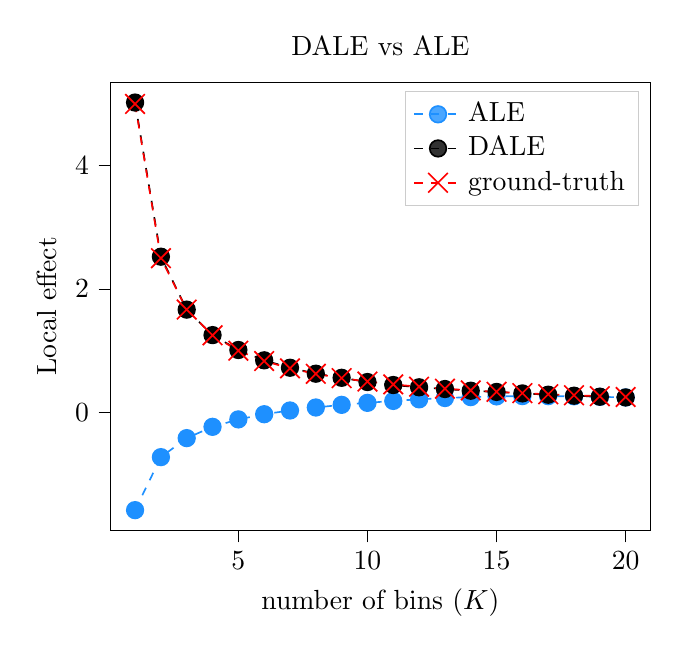
\begin{tikzpicture}

\definecolor{darkgray176}{RGB}{176,176,176}
\definecolor{dodgerblue}{RGB}{30,144,255}
\definecolor{lightgray204}{RGB}{204,204,204}

\begin{axis}[
legend cell align={left},
legend style={fill opacity=0.8, draw opacity=1, text opacity=1, draw=lightgray204},
tick align=outside,
tick pos=left,
title={DALE vs ALE},
x grid style={darkgray176},
xlabel={number of bins \(\displaystyle (K)\)},
xmin=0.0499999999999999, xmax=20.95,
xtick style={color=black},
y grid style={darkgray176},
ylabel={Local effect},
ymin=-1.91455718867646, ymax=5.35298172476343,
ytick style={color=black}
]
\addplot [semithick, dodgerblue, dashed, mark=*, mark size=3, mark options={solid}]
table {%
1 -1.58421451079283
2 -0.724791391897207
3 -0.416931226166923
4 -0.233523181012335
5 -0.113002110067188
6 -0.0293908088400257
7 0.0312305603326059
8 0.0797401389995273
9 0.12275670716894
10 0.155053447821085
11 0.186088568383995
12 0.211864987771331
13 0.233108878251814
14 0.247869171569635
15 0.259566596177554
16 0.264108921400541
17 0.263569771086526
18 0.260892620884744
19 0.252751953555994
20 0.242460730712491
};
\addlegendentry{ALE}
\addplot [semithick, black, dashed, mark=*, mark size=3, mark options={solid}]
table {%
1 5.0226390468798
2 2.52393513932938
3 1.66605371806444
4 1.25321810135996
5 1.01182618748851
6 0.844347970008633
7 0.723984251300441
8 0.627612080163916
9 0.560862770386464
10 0.492398374084428
11 0.444051023514039
12 0.4070407257714
13 0.379038857924861
14 0.351678147881759
15 0.331857705495926
16 0.307844113455479
17 0.286910008925387
18 0.270908782811331
19 0.254748495290572
20 0.24246073071272
};
\addlegendentry{DALE}
\addplot [semithick, red, dashed, mark=x, mark size=5, mark options={solid}]
table {%
1 5
2 2.5
3 1.66666666666667
4 1.25
5 1
6 0.833333333333333
7 0.714285714285714
8 0.625
9 0.555555555555556
10 0.5
11 0.454545454545455
12 0.416666666666667
13 0.384615384615385
14 0.357142857142857
15 0.333333333333333
16 0.3125
17 0.294117647058824
18 0.277777777777778
19 0.263157894736842
20 0.25
};
\addlegendentry{ground-truth}
\end{axis}

\end{tikzpicture}
}
  \caption[Example comparison]{(Left) The black-box function \(f\) of
    Section~\ref{sec:4-3-robustness}. (Right) Estimation of the local
    effect of the first bin for DALE and ALE, for varying number of
    bins \(K\).}
  \label{fig:example-different-bins}
\end{figure}
